\documentclass[12 pt, a4paper]{thesis}
\usepackage[left=40mm, top=20mm, bottom=20mm, right=10mm]{geometry}
\usepackage{graphicx}
\usepackage{array}
\usepackage{amssymb}
\usepackage{multicol}
\usepackage{amsmath}
\usepackage{amsthm}
% - - - - - - - - - - - - - - - - - - - - - - - - - - - - - - - - - - - -
\graphicspath{{./graphics/}}
\author{Toan, Truong Thanh}
\title{Realization of  Sensor-Shoe}
\makeindex
\begin{document}

\begin{titlepage}
	\centering
	\includegraphics[width=0.45\textwidth]{FRA_1.jpg}\hfill
	\includegraphics[width=0.45\textwidth]{VGU.jpg}\par\vspace{1cm}
	\vspace{1cm}
	{\scshape\Large Bachelor thesis\par}
	\vspace{1.5cm}
	{\huge\bfseries Realization of a SensorShoe\par}
	\vspace{2cm}
	{\Large\itshape Truong Thanh Toan\par}
	\vspace{1cm}
	{\Large\itshape Matriculation: 1185050\par}
	\vspace{1cm}
	\includegraphics[height = 70mm]{shoe.jpg}
	\vfill
	{\LARGE Supervised by:\par}\vspace{1cm}
	Prof. Dr. Sven \textsc{Kuhn}\par
	Dr. Heiko \textsc{Hinkelmann}

	\vfill

% Bottom of the page
	{\large \today\par}
\end{titlepage}
\thispagestyle{empty}

\vfill\noindent
\tableofcontents
\listoffigures
\listoftables
\chapter*{acknowledgement}
This section was devoted to address thank to all the people who have helped with this work. It is more polite and expressive that first person pronoun was used here.\\
Fristly, I want to give my thanks to my family and friends, who had been very closed and helpful during my stay in Germany. Big thanks to my instructor Dr.Kuhn for his instructions during both the senior and thesis. Thank the Electronic Workshop: Mr.Hartmann and Mrs.Hepp for helping me with all the PCBs design and manufacturing. I kindly thank Mr.Mansooji for giving me access to the room where I can work on this project. Best regards for Mr Hoang An,Phan whose thesis work on an alike system, which had motivated the execution of this work. 
\chapter*{Disclaimer}
All the works in this this thesis, if not stated were done by the student conducting the project. There were a lot of undone tasks throughout the work, all were stated. Human, or subjects mentioned in the work are considered to have walking abilities either good or bad, as for the scope of the work of studying about Gait, or walking. This work focuses on the study of gait rather than excluding the disabled subjects.
\vspace{30mm}
\begin{multicols}{2}
\centering

------------------------------ \\

Date\\ 

------------------------------ \\
Truong Thanh Toan\\


\end{multicols}
\pagebreak 
\begin{abstract}
	This thesis introduce about data collection of gait in foot area, with an aid of a Sensor-Shoe system on the left foot. The data includes acceleration, angular velocity and ground-reaction force\footnote{usually called \textit{"plantar force"} in other texts}.
Throughout the text, software application of the detecting algorithm, and the manufacturing of the hardware are covered. In the end a full-fledged SensorShoe system was realized and tested.
\end{abstract}
%===================================================================
\chapter{Introduction}
	Human gait is very important to everyday life because walking, or commuting is a everyday task. But it was not a big deal until one suffers from its absence, or abnormalities from not using it right. These sudden negative shift in walking gait can cause instant discomforts and lower life quality. In the other hand improving one's gait also remarkably aid for a happier, healthier life. Gait analysis has been in great help for recognizing and dealing with many of different diseases and symptoms regarding skeletal structure, muscular movement and many other areas for decades. This thesis was dedicated to give insights to the design of a system that collects data for Gait Analysis. The system can be assumed as a Sensor-aided Shoe that can collect the raw gait data around the foot area and send the data to a separate computer for processing.  
\chapter{Theoretical Background}
\section{Gait Analysis}
Movement of animals that includes motion of limbs during locomotion through a supported, solid ground is called Gait: walking, running, galloping, climbing stairs ... . For example, Walking Gait Analysis is the study about Human posture and gestures, during the action of walking. These studies include the work of careful observation, sometimes with aid of measuring instruments\cite{whittle} by experienced doctors and physical therapists. The Observation can then give clue about the cause, the treatment method or the cure for the suspected illness. Because gait depends on a lot of different factors, Gait Data includes a wide range different properties which can be found throughout the body: leg muscle contraction, angular velocity of foot, balance of the body when walking, foot ground reaction force, body center of mass, ... .\\
However, the average person doesn't think much about his/her gait. Walking is "used" everyday as a mean of commuting and it becomes too normal and common that few people (ones who aren't familiar with gait analysis) give attention to it. Therefore, there can be unexpected consequences when the subjects are exposed to bad gait, gesture without noticing or with faint awareness. Abnormal Gait or asymmetrical gait are a potential risk as in long term, they may lead to bigger health issues. One of the cause includes altering our gait for a long time period e.g. to avoid pain when we have injuries\cite{tekscan}. Gait analysis can help avoid, or neutralize these risks with the help of physical therapy, e.g in the regenerative process of the patient.\\
\section{Gait Cycle}
\begin{figure}[hbt!]
\begin{center}
\includegraphics[width = 150mm]{gait_cycle.jpg}
\caption{Human bipedal gait analysis \cite{gaitcycle}}
\end{center}
\end{figure}
For human beings, the study focus primarily on bipedal gait analysis, which literally means locomotion with 2 limbs. The pedal here can be regarded as the foot. A gait cycle, or a stride is the shortest repeatable series of motion that the gait possesses during a normal commutation, see Fig.2.1.\\
A Gait cycle consists of different phase in between and consecutive events in the time domain. Figure 2.1 show a complete and clear demonstration of a normal human walking gait cycle.\\
For the concise explanation, Classic Gait Term were used here.
\begin{itemize}
\item{Heel Strike is considered the initial contact of the foot with the ground. This event is when the heel makes first contact with the surface and exerts force in the heel area.}
\item{Foot Flat is the event when the entire foot is on the ground, making full plantar contact force on the surface. }
\item{Midstance is the event when the foot bears the whole body force while the foot is still in its full plantar contact}
\item{Heel Off releases some force on the selected foot leaving force only in the Toe area}
\item{Toe off release all the force, leaving the foot with no ground reaction force and begin air time.}
\item{Midswing shows large anglar velocity and acceleration, but no Ground reaction force. The swing ends with a Heel Strike, beginning a new walking gait cycle.}
\end{itemize} 
The Gait Cycle suggests an example of data set that can be extracted : time stamps of gait event\cite{Shuo} use angular velocity and acceleration in the sagittal plane of the shoe. Selection of data and the processing direction should be first done to narrow the work.\\
However, due to the lack of research during the work and the limited time frame, the hardware part was prioritized to be manufactured first. This was done to take as many data as possible and put them into visualization. From the observation of the raw data, a better understanding could be achieved before taking a narrower, objective approach. Then it comes with an option to trim down the data to a more compact design and processing. 
\section{Other Work}
Though the idea of a Sensor-Shoe may seem uncommon, there have been a tremendous amount of others who have dived into the same area. These works include wearable systems on the leg and foot area: wearable system to get shank orientation\cite{Monaghan},a thick insole to carried the pcb inside to control an exoskeleton\cite{Kim}, embedded sensor in a load-helping exoskeleton for Joint Angle detection\cite{Zhang}, a ForceShoe with force sensor underneath\cite{Mohamed}, a case installed on the shoe for Angular velocity and acceleration\cite{Shuo}, a in-heel Accelerometer shoe\cite{Nilsson}. The picture was not included because there were no permission from the writer, please search for the reference in case one needs more information.\\
\section{OpAmp}
The Operation Amplifier should be a fundamental step stone for anyone who practices engineering. This section is dedicated for the review of the subject and an explanation to the theory that were applied in this work. Instead of digging through the theory of field and transistor that lies below the concept, this section intend to show the reader the usage of OpAmp in this work.\\
An Operational amplifier is a device which was used to amplify the voltage difference at the input gate. The bare operation, which employs usage of Open Loop Gain put a very large coefficient to the voltage (in term of 1,000,000 (120dB) or more). Scarce application that include OpAmp take advantage of this feature. So mostly, OpAmps are used with feedback from the output. The equation when having this concept applied is feasible and useful.\\
\begin{figure}[hbt!]
\centering
\includegraphics[width=100mm]{OpAmp_1.png}
\caption{Bare OpAmp with no feedback}
\end{figure}
So in this section, application, or 3 common OpAmp circuits with feedback will be discussed. To start with there are two main rules that must be remember when working with OpAmps:
\begin{itemize}
\item{There are no (very little) current that flows through the two input pin}
\item{The Differential Input Voltage is Zero as V1 = V2 = 0 (Virtual Ground)}
\end{itemize}
These two rules will later explain the 3 circuits. Firstly, the inverting amplifier is put into discussion.\\
\begin{figure}[hbt!]
\centering
\includegraphics[width=100mm]{OpAmp_2.png}
\caption{Inverting Amplifier circuit}
\end{figure}
From point x, $V_2-V_1=0, V_2=V_1=0$, then using node current here:
\begin{equation}
\begin{split}
I_{in} &=I_{V_{1}V_{2}}+I_F\\
I_{V_{1}V_{2}} &=0 \:(by\: rule\: 1)\\
I_{in} &=I_F\\
\frac{V_{in}}{R_{in}} &=-\frac{V_{out}}{R_F}\\
V_{out} &=-\frac{R_F}{R_{in}}V_{in}
\end{split}
\end{equation}
\vspace{10mm}
Second the non-inverting amplifier circuit is examined.
\begin{figure}[hbt!]
\centering
\includegraphics[width=100mm]{OpAmp_3.png}
\caption{non-inverting amplifier}
\end{figure}
\\Consider the pink line through the two resistors. This setup forms a voltage divider between $V_{OUT}$. From that, the following calculation can be carried out:\\
\begin{equation}
\begin{split}
V_1 &=V_{OUT}\frac{R_F}{R_2+R_F}\\
V_{IN} &=V_1 \:(from rule 2)\\
V_{IN} &=V_{OUT}\frac{R_F}{R_2+R_F}\\
V_{OUT} &= (\frac{R_2}{R_F}+1)V_{IN}
\end{split}
\end{equation}
\\The application that was used was a special case derived from this circuit, when $R_F=0$ and $R_2=\infty$. This setup is called a Non-Inverting Voltage Follower:\\
\begin{figure}[hbt!]
\centering
\includegraphics[width = 100mm]{OpAmp_4.png}
\caption{Non-Inverting Voltage Follower}
\end{figure}
\begin{equation}
V_{OUT} = V_{IN}
\end{equation}
The result is also regarded as a impedance changer, because the voltage was reserved unchanged in the output circuit, regardless of the system impedance. The circuit then keep the resistance of the load from affecting the voltage. The usage of this circuit in the SensorShoe system was to make referent voltage to drive the Force Board sensor conditioning circuit.\\
The final circuit used in this thesis was the differential amplifier.\\
\begin{figure}
\centering
\includegraphics[width = 100mm]{OpAmp_5.png}
\caption{Differential Amplifier}
\end{figure}
Considering the 3 currents $I_1,I_2,I_f$:
\begin{equation}
\begin{split}
I_1 = \frac{V_1-V_a}{R_1},\:I_f &=\frac{V_a-V_{OUT}}{R_3},I_2=\:\frac{V_2-V_b}{R_2}\\
V_a &=V_b = V_2\frac{R_4}{R_2+R_4}\\
I_1 &=I_f\\
\frac{V_1-V_a}{R_1}&=\frac{V_a-V_{OUT}}{R_3}\\
V_{OUT}&=V_a-\frac{R_3}{R_1}(V_1-V_a)\\
V_{OUT}&=V_2\frac{R_4}{R_2+R_4}-\frac{R_3}{R_1}(V_1-V_2\frac{R_4}{R_2+R_4})\\
V_{OUT} &= V_2(\frac{R_4}{R_2+R_4})(1+\frac{R_3}{R_1})-\frac{R_3}{R_1}V_1\\
or\:\:V_{OUT} &= V_2\frac{R_4(R_1+R_3)}{R_1(R_2+R_4)}-\frac{R_3}{R_1}V_1
\end{split}
\end{equation}
\\In the special case , to make it a Linear Subtractor Amplifier, $R_4 = R_3$ and $R_2 = R_1$ draws the equation:
\begin{equation}
V_{OUT}=\frac{R_3}{R_1}(V_2-V_1)
\end{equation}
\\For $R_1=R_2=R_3=R_4$, the circuit is considered as a \textit{Unity Gain Differential Amplifier} or a \textit{Symmetric Differential Amplifier:}
\begin{equation}
V_{OUT} = V_2-V_1
\end{equation}
\\These result will be later reviewed with application in the ShoeSensor System. A more in-dept material about OpAmp, which this section had referred to can be found at \cite{ETut}. This web page should provide a better read on OpAmp if one found the motivation. 
%including other work of the shoe
%what is the preferred data for the analysis
%what method has been used
\chapter{Realization of the System}
\section{General}
The Sensor-Shoe system can be described from "General realization of the System Building Blocks" in Figure 4.1. To be simple, Hardware part is the setup of the System on the shoe. The Software part runs on a PC (laptop) as a program. The Arrows represent the designed logics: 
\begin{itemize}
\item {Green arrow is the transmission medium (Wifi 802.11 b/g/n) in a LAN (local area network) hosted by the Laptop.}
\item{Red arrows are power supplies.}
\item{Yellow arrows are data way within the Hardware part or the Software part}
\end{itemize}

\begin{figure}[ht]	
\begin{center}
\includegraphics[width = 150mm]{ROTS_General.png}
\caption{General realization of the System Building Blocks}
\end{center}
\end{figure}
The following sections in this chapter are devoted for demonstrating the design of the System block to block. Any theoretical knowledge are kept later in the Appendix chapter for the compactness of the read.
\pagebreak
\section{Hardware}
In this Section, The design and manufacturing of the PCBs are covered, including schematics and Board (EDA Autodesk Eagle 9.4.3). Board Drawing specification:
\begin{itemize}
\item{all drill was 1.1 mm, including 0,8mm Vias }
\item{Copper pour isolation was 0,8mm }
\item{All distances, except the distance between 2 pin of the LMV324 are $\geqslant$ 0.8mm}
\item{routing copper tracks = 0.6 mm}
\item{All SMDs are installed on one side}
\end{itemize}
All of the THT devices' footprints was redesigned or made new from eagle Library. The other footprint was redrawn from online source (Wemos D1 R1, MT3608, ADS1115) library\cite{diy}. All of them are checked again with a digital caliper (resolution 0.1mm) with respect to real received devices.
Each schematic, BOM and board design are shown at the last part of each board section for reference.
%========================================================================
\subsection{Force Board}
\begin{figure}[hbt]
\begin{center}
\includegraphics[width = 100mm]{A301_spec.png}
\caption{Flexiforce A301 spec, from Tekscan datasheet}
\end{center}
\end{figure}
The name \textit{"Force Board"} here implies the usage of a signal conditioning board for the force sensors. The insole, where the Flexiforce A301 force sensors are installed, is located in the shoe. The Force Board converts the signal voltage received from the insole - vertical force pressure from the sensor to the appropriate voltage scale for the ADC. The converted signals were then fed to the interface between the force board and the data board (6 wires) to be read by the ADC ADS1115. This section explain why force board is needed and its current design. 
\subsubsection*{LMV324}
LM324 is a general, low power OpAmp, powered by 2.7V to 6V source and support both single and double supply. This IC was used in replacement of the LM358 in the prototype - breadboard version. The OpAmps in LMV324 were used in this Project as Voltage follower, inverting Amplifier and Differential Amplifier\footnote{see OpAmp in Theoretical Background}. 
\subsubsection{Flexiforce A301}
The Flexiforce A301 sensor from TekScan were used to measure ground reaction force under the foot.  These sensors are claimed from Tekscan to have a linear conductance behavior with respect to increase in applied pressure. That means $C=\frac{1}{R_s}\propto F_{applied}$ \cite{silverA301}.\\
% - - - - - - - - - - - - - - - - - - - - - - - - - - - - - - - - - - - 
\begin{figure}[hbt!]
\begin{center}
\includegraphics[width=120mm]{FlexA301CR.png}
\end{center}
\caption{Sensor behavior, figure from Tekscan\cite{silverA301}}
\end{figure}
% - - - - - - - - - - - - - - - - - - - - - - - - - - - - - - - - - - - -
The circuit to condition the Sensor for exploitation of this linearity is recommended from Tekscan as in Figure 4.3. This is an inverting amplifier, the output voltage is a multiplication of -Vt with a linear coefficient $\frac{1}{R_S}$, which results in a linear voltage behavior with respect to the applied force on each sensor. 
\\However,$V_t=-1V$ was not available in the current design as a negative voltage. In this design the usage of a virtual ground(VG) was applied.\\
% - - - - - - - - - - - - - - - - - - - - - - - - - - - - - - - - - - - -
\begin{figure}[hbt!]
\begin{center}
\includegraphics[width = 150mm]{FlexA301Cir.png}
\end{center}
\caption{Recommended circuit from Tekscan Flexiforce A301 Datasheet}
\end{figure}
% - - - - - - - - - - - - - - - - - - - - - - - - - - - - - - - - - - - -
Alternations in the Recommended Circuit in Fig. 3.4 were made to fit for the design of the full system:
% - - - - - - - - - - - - - - - - - - - - - - - - - - - - - - - - - - - -
\begin{itemize}
\item{Usage of LMV324IDT - SO14 instead of MCP6004}
\item{$V_T = V_- + VG$}
\item{$VG$ connected to non-inverting pin of the OpAmp}
\item{The output is $VG+(-(V_- + VG - G)*\frac{R_F}{R_S})=VG+V_-*\frac{R_F}{R_S}$}
\item{A voltage offset omitting circuit (to cancel VG part) was applied for higher resolution of the ADC ADS1115\footnote{discussed later in Data Board} reading. For this job an additional symmetric differential amplifier\footnote{for detail of the differential amplifier please see the OpAmp section} was used, See Fig. 3.5. The Ouput voltage now should be $V_{OUPUT} = V_1-V_2$ with $V_1=VG+V_-*\frac{R_F}{R_S}$ and $V_2=VG-V_{offset}$. This makes $V_{OUTPUT}=V_{offset}+V_-*\frac{R_F}{R_S}$}
\end{itemize}
% - - - - - - - - - - - - - - - - - - - - - - - - - - - - - - - - - - - -
\begin{figure}[hbt!]
\begin{center}
\includegraphics[width = 120mm]{Diff.png}
\end{center}
\caption{Symmetric Differential amplifier}
\end{figure}
% - - - - - - - - - - - - - - - - - - - - - - - - - - - - - - - - - - - -
In this way the linear pattern was applied without generating a negative voltage source $V_T$.\\
The supply voltage of the LMV324 is 2.7 to 6V as in the datasheet\cite{lmv324}.Although we need the largest voltage as possible, only 5V power supply was applied to the IC power supply $VHIGH$ for safety. Then the VG is realized as half $VHIGH/2$ of 5V, or 2.5V. The earlier experiment on a testboard with a slightly different amplifier LM358 showed a small offset of about 0.8V at output, any meaningful output signal below 0.8v will be pull to 0.8V. For this reason an offset voltage was kept changeable if another OpAmp should be used. Even the LMV324 was designed to have rail-to-rail performance, which means it can get as 0V offset voltage, this part is still kept in the circuit to make the design flexible. Thus can the design be set to 0V offset voltage when convenient.\\  	
Back to the board design, there will be 6 force sensors in total. Each of these sensors require 2 OpAmps for their conditioning. That makes a total of 12 OpAmps or 3 LMV324 (each has 4 OpAmps). The rather same explanation will be covered again in the Power Board when explaining the voltage references. The Force Board has 3 interfaces out, see the Schematic of the board in Fig. 3.5:
% - - - - - - - - - - - - - - - - - - - - - - - - - - - - - - - - - - - -
\begin{figure}[hbt!]
\begin{center}
\includegraphics[width = 150mm]{ForceSch.png}
\caption{Force Board Schematic}
\end{center}
\end{figure}
% - - - - - - - - - - - - - - - - - - - - - - - - - - - - - - - - - - - -
\begin{itemize}
\item{5 pins - Input Voltage : Takes the Ground and the required voltages from the Power Board}
\item{6 pins - Board Output : 6 $V_{OUTPUT}$ from the sensors, after conditioning}
\item{7 pins - Sensor Input : 6 raw connections from the the Sensor and the $V_T$ input to the sensors, these connects to the Insole in the shoe }
\end{itemize}  
% - - - - - - - - - - - - - - - - - - - - - - - - - - - - - - - - - - - -
The Board routed from the design and the BOM was shown below in Fig. 3.6 and Tab. 3.1.
% - - - - - - - - - - - - - - - - - - - - - - - - - - - - - - - - - - - -
\begin{figure}[hbt!]
\begin{center}
\includegraphics[width = 10cm]{ForceBrd.png}
\caption{Force Board Parts arrangement (Copper Pour hidden for clear observation)}
\end{center}
\end{figure}
% - - - - - - - - - - - - - - - - - - - - - - - - - - - - - - - - - - - -
\begin{table}[hbt!]
\begin{center}
\begin{tabular}{| m{0.7cm} | c | m{2.5cm} | c | m{4cm} | m{4cm} |}
\hline
Qty & Value & Device & Package & Parts & Description\\
\hline
1 & & PINHD-1X5 & 1X05 & JP1 & PIN HEADER\\
\hline
1 & & PINHD-1X6 & 1X06 & JP2 & PIN HEADER\\
\hline
1 & & PINHD-1X7 & 1X07 & JP3 & PIN HEADER\\
\hline
6 & 100k & $R-EU_R0805$ & R0805 & R9, R10, R19, R20, R29, R30 & RESISTOR ,European symbol\\
\hline
24 & 330 & $R-EU_R0805$ & R0805 & R1, R2, R3, R4, R5, R6, R7, R8, R11, R12, R13, R14, R15, R16, R17, R18, R21, R22, R23, R24, R25, R26, R27, R28
& RESISTOR, European symbol\\
\hline
6 & 47pF & $C-EUC0805$ & C0805 & C1, C2, C3, C4, C5, C6 & CAPACITOR, European symbol\\
\hline
3 & & LMV324M & SO14 & IC1, IC2, IC3 & Quad General Purpose, Low Voltage, Rail-to-Rail Output Operational Amplifiers\\
\hline
\end{tabular}
\end{center}
\caption{Bill of materials - Force Board}
\end{table}
% - - - - - - - - - - - - - - - - - - - - - - - - - - - - - - - - - - - 
\pagebreak
%========================================================================
\subsection{Power Board}
This Board Job is to generate all used voltage level of the whole Hardware part. The Included Voltage level can be listed with functions in Table 4.1 . Some of the Voltages listed in this section needs reference from other Board to see their functionalities (VG, VG-1, VG/2 from the Force Board section).\\
The Power Board is designed for the ability to easily alter the Voltage, in case a new component or design should be considered for test.
% - - - - - - - - - - - - - - - - - - - - - - - - - - - - - - - - - - - - 
\subsubsection*{MT3608 DC-DC converter}
A Dc-Dc converter was used to convert the voltage from a 3.7V 18650 battery to 5V, this voltage is used as the VHIGH for the entire system.
This DC-DC converter was included in the design mainly for the purpose of testing and changeability. The module can pass a very high current Max 2A. or working voltage: input 2-24V, output of max 28V. Overall it can satisfy a wide range of electronic projects.
\begin{figure}[hbt!]
\centering
\includegraphics[width = 120mm]{MT3608.png}
\caption{MT3608 DC-DC converter}
\end{figure}
% - - - - - - - - - - - - - - - - - - - - - - - - - - - - - - - - - - - -
\subsubsection{Board Design}
The following section discuss about the board design, the arrangement of the parts and how the generation of the voltage works. For the need to review the design, the Bill of Material is listed in table 3.3, the Schematic in Fig. 3.9 and the Board in Fig. 3.10.\\
\begin{table}[hbt!]
\begin{center}
\begin{tabular}{ | m{2cm} | m{1cm}| m{12cm} |} 
\hline
Voltage & Value & Functionalities\\
\hline
Source & 3.7V & Power supply from the 18650 Battery.\\
\hline
VHIGH & 5.0V & Output from the DC-DC boost converter MT3608, powers the module boards: ADS1115, WEMOS D1-R1\footnote{Esp8266-12w wifi module}, MPU9250 and the LMV324 Force Sensor Conditioning Board. \\ 
\hline
VG & 2.5V & Virtual Ground to exploit the operation of the Operational Amplifier VHIGH/2 \\ 
\hline
VG-1 & 1.5V & offset voltage for substracting the final output to get the most data\\
\hline
VG/2 & 1.2V & input voltage for the Force Sensor Flexiforce A301 \\
\hline
\end{tabular}
\end{center}
\caption{List of Used Voltage for the System}
\end{table}
% - - - - - - - - - - - - - - - - - - - - - - - - - - - - - - - - - - - -
From the output power source of 5V, other voltages were generated by using voltage divider and stabilized by the non-inverting voltage follower operation of one LMV324 OpAmp. In the current design there were 3 voltage that can be altered for when needed: VHIGH (the ouput power), VG-1, and VG/2. VHIGH can be easy changed by rotating the trimmer on the MT3608 .This feature is useful when another Power Supply is used instead of the 18650 battery, as long as the voltage rating is smaller than 5V. VG was the virtual ground used for the operation of the OpAmp. In order not to used the negative voltage, a VG was applied to become a ground reference point for the oscillating of the OpAmp $0-VG-VHIGH$ instead of $-VG-0-VG$ or $-VHIGH/2-0-VHIGH/2$. VG was sufficiently chosen to be half of VHIGH, this voltage was created using a voltage divider of two identical resistor. Neglecting the tolerance, output voltage should be close enough to VG/2, the voltage was then fed through a non-inverting voltage follower to isolate it from the output load. \\
The two other voltages VG/2 and VG-1 were named with ambiguity. But due to their usage from the senior project, the name were kept to maintain continuity. \\
The VG/2 voltage function was to create the pseudo negative voltage with respect to VG (which means it only needs to be smaller than VG). The negative voltage then have the value of $V_{-}=-VG+VG_{/2}<0$ for the OpAmp input. It is important that $|V_{-}|$ got large enough for the signal output to be clear and measurable in range of $0V$ to $3V$. The calibration of$VG_{/2}$ can be done through rotating trimmer $R6$.\\
$VG_{-1}$ voltage is the offset subtractor to neutralized the usage of the virtual ground. After going through the Inverting Amplifier, the signal consisted of two parts: the amplified signal and the addition of the virtual ground $VG+V_{-}\frac{R_F}{R_S}$. With the usage of the Symmetric Differential Amplifier $V_{OUT} = V_2-V_1$, $VG_{-1}$ acts as a subtractor to take as much as possible $VG$ out of the signal with respect to real ground.
\begin{equation}
VG+V_{-}\frac{R_F}{R_S} - VG_{-1} = 1V + V_{-}\frac{R_F}{R_S}
\end{equation}
\\The $1V$ was from the prototype time of the system, when the LM358, instead of LMV324 was used. The LM358 during operation always output an fix lower threshold of around 0.8V. This means that if the $VG-VG_{-1}<0.8V$, a part of the signal will be lost. Thus $VG_{-1}$ had been chosen to be equal to $VG-1V$, to generate the $1V$ offset separating the signal region with the lower threshold $0.8V$. However LMV324 has the rail-to-rail voltage feature, which means it can get to the lower threshold of $0V$ ($-0.2V$ in the datasheet). This enables the full separation of the output signal from $VG$. Therefore, $VG_{-1}$ can be set near or equal to $VG$, $VG_{-1}\rightarrow VG$. For safety, the current setting of the lower threshold for the SensorShoe was $0.5V$, or $VG_{-0.5}$. The option to calibrate $VG_{-1}$ is to turn the trimmer $R5$. 
% - - - - - - - - - - - - - - - - - - - - - - - - - - - - - - - - - - - -
\begin{table}[hbt!]
\begin{center}
\begin{tabular}{| m{0.3cm} | m{2cm} | m{3.2cm} | m{2.6cm} | m{2.4cm} | m{3cm} |}
\hline
Qty & Values & Device & Package & Parts & Description\\
\hline
1 & & CPOL-EUE2.5-7 & E2,5-7 &C4 & POLARIZED CAPACITOR, European symbol\\
\hline
8 & & PINHD-1X1 & 1X01 & JP1, JP2, JP3, JP4, JP5, JP6, JP7, JP8 & PIN HEADER\\
\hline
3 & & PINHD-1X2 & 1X02 & SOURCE, SOURCE1, SWITCH & PIN HEADER\\
\hline
$1$ & & $PINHD-1X5$ & $1X05$ & $OUT_FORCE$ & PIN HEADER \\
\hline
2 & 100k & R-TRIMM3006P & RTRIM3006P & R5, R6 & Trimm resistor\\
\hline       
2 & 10k & $R-EU_R0805$ & R0805 & R3,R4 & RESISTOR, European symbol\\
\hline
2 & 47uF & C-EUC0805 & C0805 & C1, C2 & CAPACITOR, European symbol\\
\hline
1 & DC-DC-STEP-UP-MT3608 & DC-DC-STEP-UP & DC-DC-STEP-UP-MT3608 & U\$2 & DC/DC Step-Up Regulator based on MT3608 chip\\
\hline
1 & LMV324M & LMV324M & SO14 & IC1 & Quad General Purpose, Low Voltage, Rail-to-Rail Output Operational Amplifiers                                    \\
\hline
\end{tabular} 
\caption{Bill of Material for the Power Board}
\end{center}
\end{table}
% - - - - - - - - - - - - - - - - - - - - - - - - - - - - - - - - - - - -
\begin{figure}[hbt!]
\begin{center}
\includegraphics[width = 150mm]{PowerSch.png}
\caption{Power Board Parts schematic}
\end{center}
\end{figure}
% - - - - - - - - - - - - - - - - - - - - - - - - - - - - - - - - - - - -
\begin{figure}[hbt!]
\begin{center}
\includegraphics[width = 150mm]{PowerBrd.png}
\caption{Power Board Parts arrangement (Copper Pour hidden for clear observation)}
\end{center}
\end{figure}
% - - - - - - - - - - - - - - - - - - - - - - - - - - - - - - - - - - - -
\pagebreak
\subsection{Data Board}
The Data board was mainly consisted of pre-built breakout modules. These were the Wifi module Esp8266 in Wemos D1-R1, the Analog-Digital converter ADS1115, the IMU(Inertial Measurement Unit) MPU9250. This section included the brief description of the modules: what it is, which data it gives and how they communicate.\\
\subsubsection{Interfaces}
The modules communicate with each others with I2C. Esp8266-12W\footnote{was also called Wemos D1-R1 in this text} worked as a micro controller during its operation. Therefore in I2C, it take role of the master, consecutively requesting information from other modules - slave through the bus.\\
This table shows the I2C registered address for each I2C connection between the devices.
\begin{table}[hbt!]
\begin{center}
\begin{tabular}{|c|c|}
\hline
Devices & Slave Address\\
\hline
ADS1115, first 3 Sensor & 0x48\\
\hline
ADS1115, next 3 Sensor & 0x49\\	
\hline
MPU9250 & 0x68\\
\hline
\end{tabular}
\end{center}
\caption{Address of the slave- sensor devices in I2C}
\end{table}
The Data Board code uses modules, thus it came with an vast choice of Library. Conveniently, the Arduino code was written using library for the I2C and device setup. More information about the code can be found later in the software - next section of this chapter.
\subsubsection{Esp8266-12W}
A small introduction about the Esp8266 feature was keep here to raise awareness of its operation, and how it is aiding this work. \\
The Esp8266 is a common Wifi module used in plenty of Arduino, students, hobbyists projects or applications that needs the extension of Wifi. The availability and the supports it gets from the developer community make it a great, thus feasible module to be added to a wireless project. The basic module was developed by  Espressif Systems (Shanghai) and the breakout modules - usually with micro-usb to upload code, voltage regulator, or extended ADCs are made diversely by other vendors. The breakout board used in this projet is a Wemos R1 D1, which support an additional $5V$ regulator and micro USB flash boot.\\
\begin{figure}[hbt!]
\centering
\includegraphics[height = 55mm]{Esp8266.jpg}
\hfill
\includegraphics[height = 55mm]{EspSetup.jpg}
\caption{Wemos D1-R1 Wifi module, with Usb-connected to laptop on the right}
\end{figure}
\subsubsection{ADS1115}
The ADS1115 used here was a breakout board for analog-digital converter. It has an operating range of maximum ~6V reading. The use of ADS1115 as an extension provide the micro controller  like Esp8266 an upgrade from $0\rightarrow 1V-10bit$ to $-6V\rightarrow 6V-16bit$ for reading voltages. The module uses I2C bus to communicate with the Esp8266 to send the Data read. There are two features of ADS1115 that worth mentioning in the text:\\
\begin{figure}
\centering
\includegraphics[height = 70mm]{ADS1115_1.png}
\caption{ADS1115 16 bit analog-digital converter}
\end{figure}
\\
1. it can change the active range of reading to a smaller resolution. Normally, the maximum active range is kept as default $\pm 6.144/2^{15}=0.1875\: mV$ per bit for positive and negative value (sum $2^{15}+2^{15} = 2^{16}$).This active range can be altered by changing the active value in the library of the ADS1115 file Adafruit$\_$ADS1015.cpp on row 106.
\begin{figure}[hbt!]
\centering
\includegraphics[width = 150mm]{ADS1115_3.png}
\caption{changing the active range in the library file .cpp}
\end{figure}
\\The reference values can be found in Adafruit$\_$ADS1015.h of the library. However current implementation was immature and unexpected voltage spikes that overtake the maximum value may occur. For this reason, the active range was still kept at $\pm 6.144V$. Another note is that the module can only measure the voltage $\approx \pm 1V$ from the supplied voltage (2V$\rightarrow$5.5V). Not regarding this did heated up the module, e.g a 3.3V power supply reading 5V \footnote{isolating or turning off the module right away is very recommended}. 
\begin{figure}[hbt!]
\centering
\includegraphics[width=140mm]{ADS1115_4.png}
\caption{enumeration of available gain option file .h}
\end{figure}
\\
2. The ADS1115 has the ability to cooperative work with changeable I2C address. Depending on the setting of the Pin on the module when operating, it will show a different address, Fig. 3.15. This work used 2 ADS1115, at addresses 0x48 and 0x49. 
\begin{figure}
\centering
\includegraphics[height = 100mm]{ADS1115_2.png}
\caption{Available addresses configuration of the ADS1115 when operating}
\end{figure}
\pagebreak
\subsubsection{MPU9250 Inertial Measuring Unit}
The MPU-9250 is a 9-axis Motion Processing Unit. It caught a wide range in application in smart devices and wearable sensors. The MPU-9250 was delivered in a 3x3x1mm QFN package from IvenSense. It offers a great performance over cost ratio, low power comsumption and small size. The 9-axis includes 3 angle velocity $\omega\: rad/s$: Roll Pitch Yaw, 3 acceleration $a\: m/s^2$: x y z and a compass-Magnetometer.\\
\begin{figure}
\centering
\includegraphics[width = 100mm]{MPU9250.png}
\caption{MPU-9250 Breakout Board of MPU9250}
\end{figure}
\\In this project, only 6 axes of the modules was used: the acceleration(3) and the angular velocity(3) axes. The two entities value will be discussed below.\\
\begin{figure}
\centering
\includegraphics[width=100mm]{RPY.png}
\caption{Orientation of Axes of Sensitivity and Polarity of Rotation for Accelerometer and Gyroscope}
\end{figure}
1. Angle velocity:\\
These are represented in Roll(counter-clockwise in x axis direction), Pitch(counter-clockwise in y axis direction), Yaw(counter-clockwise in z axis direction). The unit for these values are rad/s. It is better that the angle velocity can be converted to the coordinate of the shoe to see each transformation in the right direction. 
2. Acceleration:\\
The 3 axis in Fig. 3.17 represent the 3 axis for acceleration x y z. Unlike the Angle Velocity, which only shows values when motion are triggered, the acceleration axes are always affected by the gravitational acceleration, which point downward to the center of the earth and approximately 9.8$m/s2$. This is to expect a non zero resting position. Another remark for this was that there is always imperfect initial orientation of the modules. Therefore The vector value $9.8m/s^2$ becomes the combination of the output from the 3 acceleration axes in resting state.\\
\begin{equation}
g = x+y+z \: (vector\: values)
\end{equation}  
\\
Then for the true, or observable acceleration data which take the shoe orthogonal coordinate system, initial calculation have  to be made to translate the x y z output.\\
It was a pity that such calculation for the data couldn't have been done in the limited duration. Frankly, the IMU itself can also be considered as a project. This work avoid diving deep into the subject by using a built-in library in Arduino IDE. 
\subsubsection{Board Design}
The next subsection show how the board was wired,  the usage of component and the current arrangement of the design.\\
The Schematic Of the Data Board is rather feasible to comprehend, see Fig. 3.11. There were not many connection between the Esp8266 - micro controller and the data collecting - ADS1115, MPU9250 modules. The feature of I2C allows the use of data transfer in the same line, so only 2 line SDA, SCL were responsible for the transferring of data in the Data Board. The other connection on this board are the power source of 5V, the setting of ADS1115 address and the routing of force sensor data to ADS1115.  \\
\begin{figure}[hbt!]
\centering
\includegraphics[width = 150mm]{DataBoardSch.png}
\caption{Schematic of the Data Board}
\end{figure}
From The Schematic, a design of the Board was developed. Instead of the bare Esp8266 the Wemos R1 - D1, which took up a little more space, was used. This was to enable the ability of the system program to be easily updated through Usb cable. A remark when designing this Board was to keep the antenna part of the Esp8266 away from the Board to avoid any electromagnetic interference that may distort the Wifi Operation.\\
\begin{figure}[hbt!]
\centering
\includegraphics[width = 150mm]{DataBoard.png}
\caption{Data Board parts arrangement (Copper pour hidden for clear observation)}
\end{figure}
The following table show the Bill of Material used for the current implementation of the Data Board.
% - - - - - - - - - - - - - - - - - - - - - - - - - - - - - - 
\begin{table}[hbt!]
\begin{center}
\begin{tabular}{| m{0.3cm} | m{1.5cm} | m{2.2cm} | m{2.6cm} | m{2.4cm} | m{3cm} |}
\hline
Qty & Values & Device & Package & Parts & Description\\
\hline
1  & MPU9250   & MPU9250 & MPU1 & & IMU \\
\hline 
17 & PINHD-1X1 & 1X01   & JP17, JP19, JP20, JP21, JP22, JP23, JP24, JP25, JP26, JP27, JP28, JP29, JP30, JP31, JP32, JP33, JP34 & PIN HEADER & Some were used as Vias because of alternation for the LPKF to work\\
\hline
1    & PINHD-1X2 & 1X02 & JP2 & PIN HEADER & VCC for the Esp8266\\
\hline
1    & PINHD-1X6 & 1X06 & JP1 & PIN HEADER & 6 sensors inputs\\
\hline 
2    & ADC-4CH-ADS1115 & ADC-4CH-ADS1115 & ADC-4CH-ADS1115 & U\$2, U\$3 & 4 Channel 16-Bit Analog-to-Digital Converter based on ADS1115 chip\\
\hline 
1    & WEMOS-D1-MINI & WEMOS-D1-MINI & WEMOS-D1-MINI & U\$4 & WEMOS D1 mini: Mini Wi-Fi Board based on ESP-8266 device \\
\hline
\end{tabular}
\end{center}
\caption{Bill of Material Data Board}
\end{table}
\subsection{Insole}
The insole is manufactured to have the same shape of an insole of a normal sneaker. To start with the design, it was not considered to be very robust, that it can be used in different kind of shoe, e.g high-heels. There were two reason for the design the time this project was carried:
% - - - - - - - - - - - - - - - - - - - - - - - - - - - - - - - - - - - - 
\begin{itemize}
\item{Availability of the shoe}
\item{A sneaker is a common, casual shoe used mainly for low, medium speed activity: walking, climbing stairs, skateboarding, ...}
\end{itemize}
% - - - - - - - - - - - - - - - - - - - - - - - - - - - - - - - - - - - -
The material choice on making the insoles where considered to enable flexibility in movement and protection of the sensors. The Flexiforce A301 takes a perpendicular force sensing direction with respect to the surface. The material thus must have the property of elastic surface but not in the vertical direction. And It was recommended to make a high friction contact between the surface and the sensing area to reduce sheer force (force with direction vector parallel with the sensing area surface ). This force can reduce sensitivity of the sensors. In this work, a recycled rubber sheet was used to make the insole\footnote{It was later found that a PVC sheet would have been a better choice, but was not available at the time this thesis was written}.\\
Steps:
% - - - - - - - - - - - - - - - - - - - - - - - - - - - - - - - - - - - - 
\begin{enumerate}
\item{cut the insole in the shape of the shoe's extracted insole}
\item{using a chalk and paint all the bottom of the foot}
\item{then use the foot to step on the insole, like normal shoe wearing}
\item{search the area with chalk dust on the rubber insole for sensors placement}
\item{mark them with a paper knife}
\end{enumerate}
% - - - - - - - - - - - - - - - - - - - - - - - - - - - - - - - - - - - 
\begin{figure}[hbt!]
\begin{center}
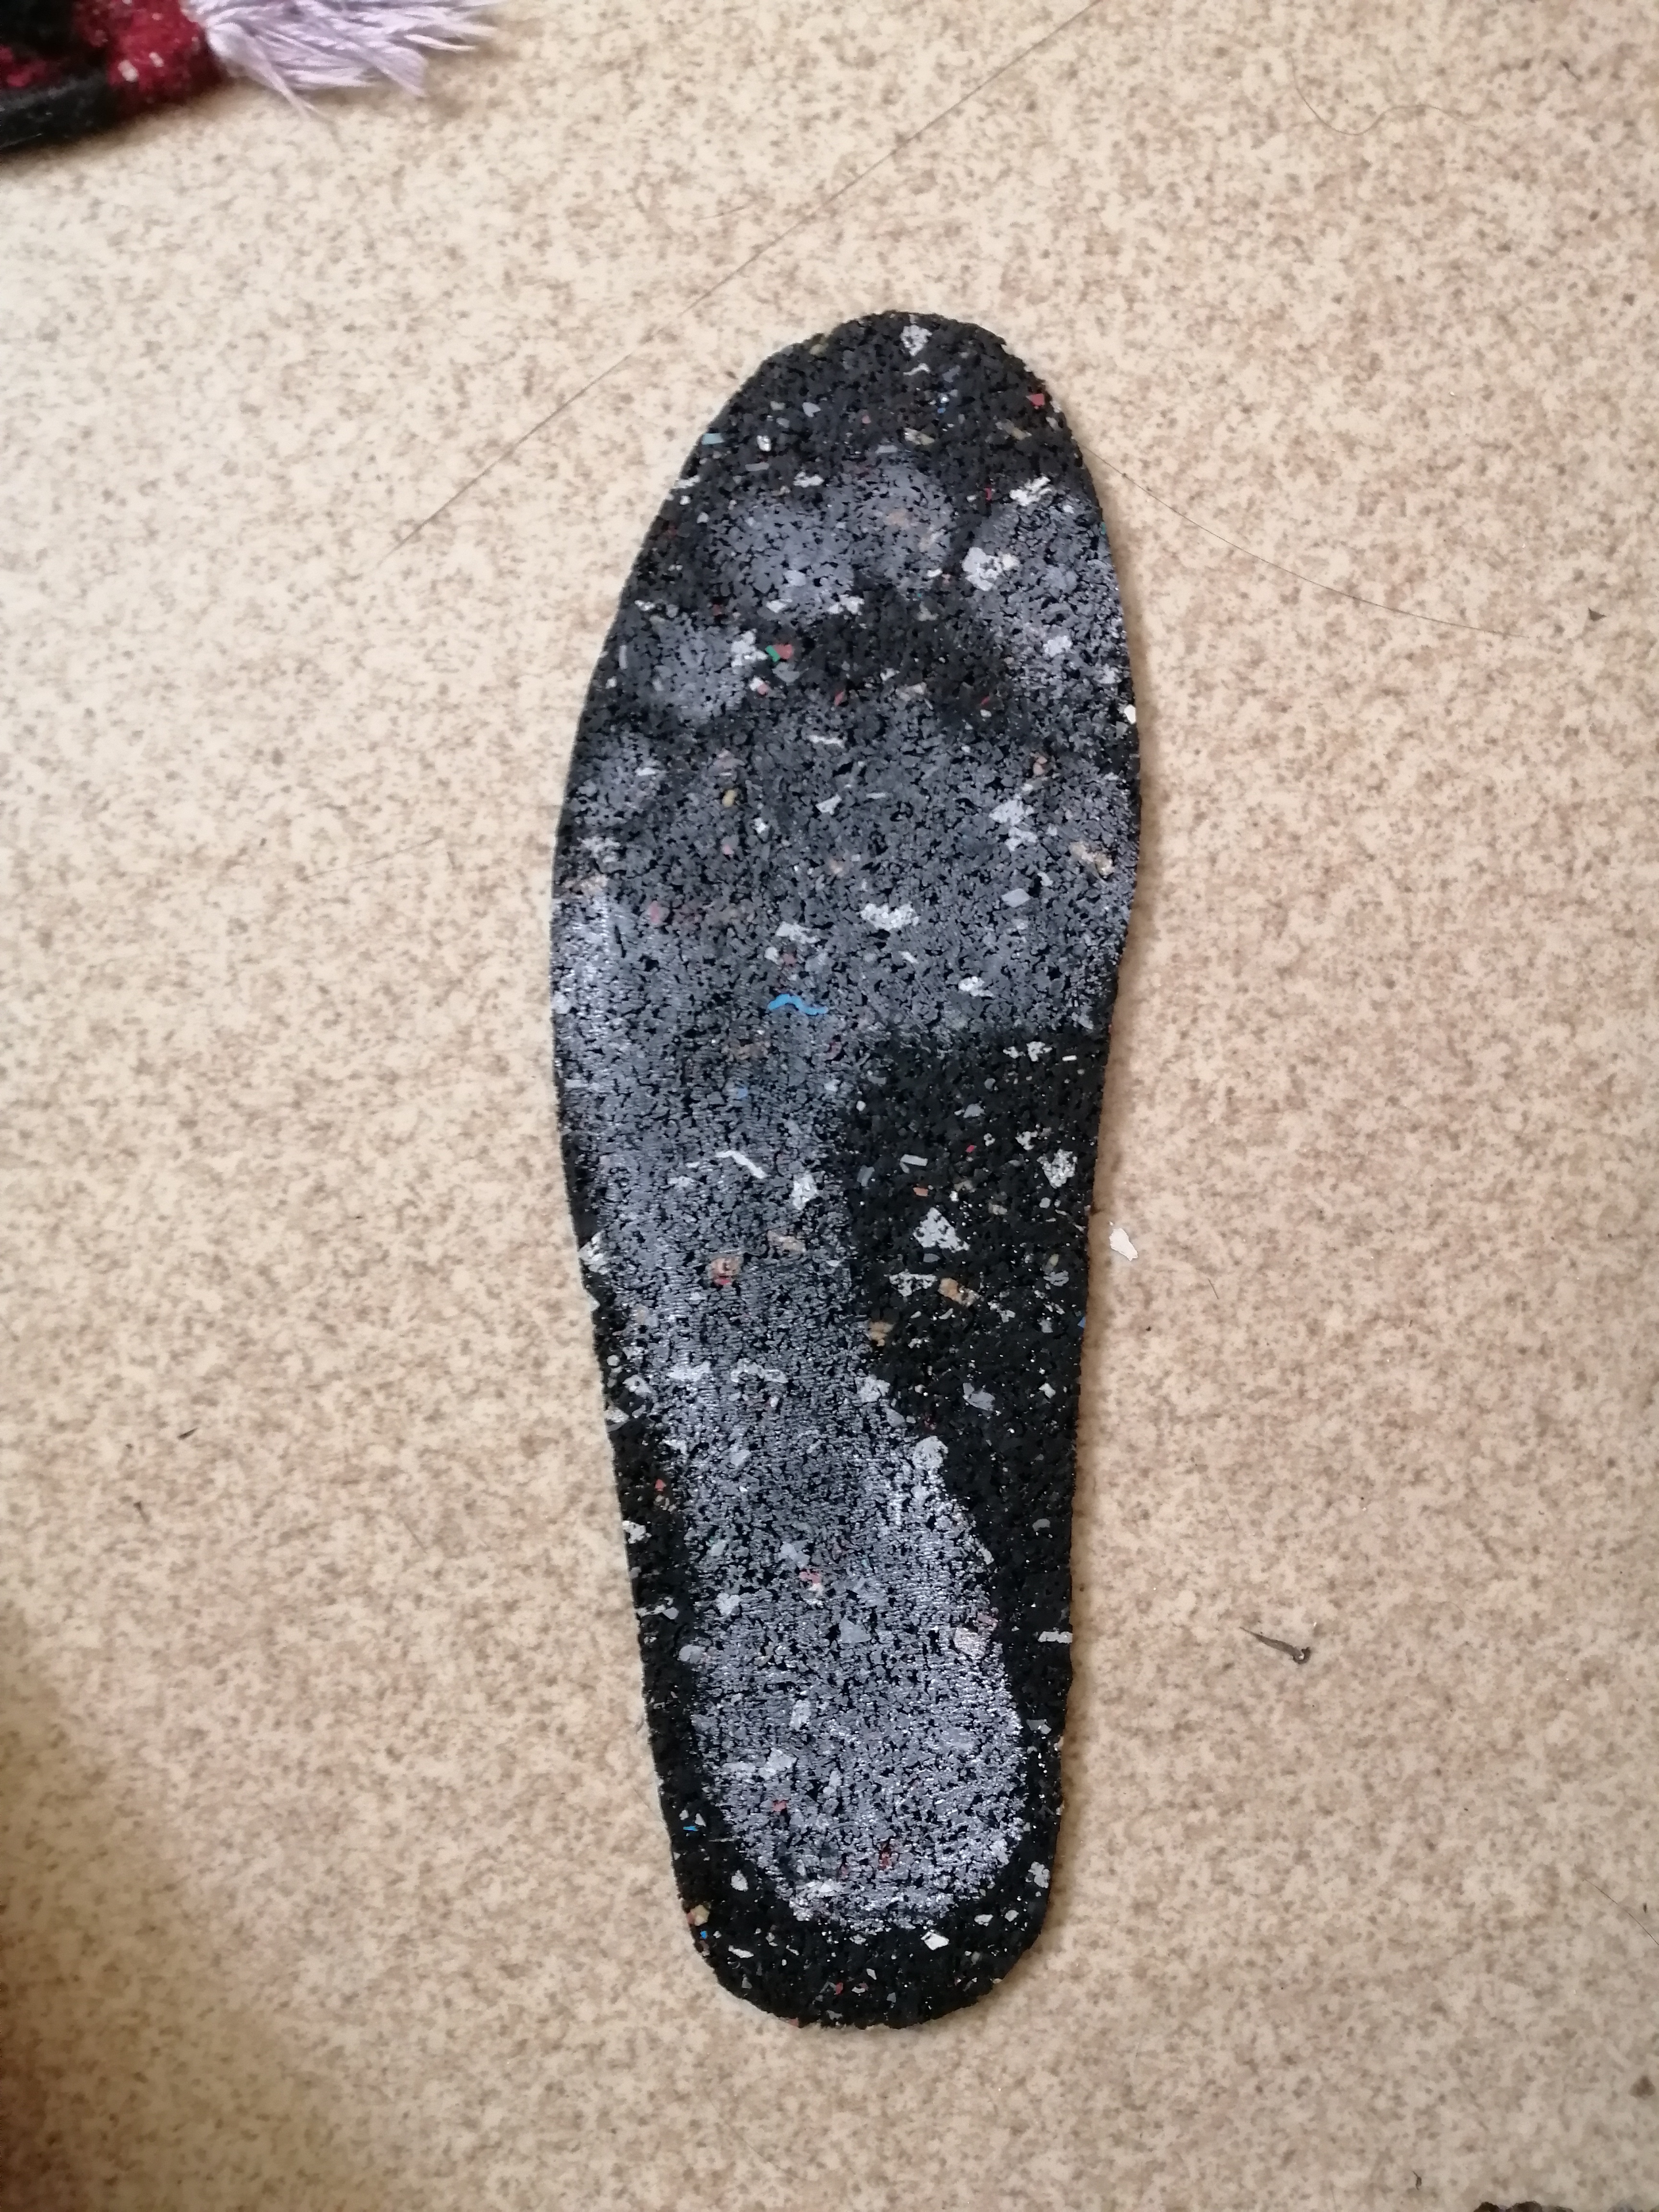
\includegraphics[width=50mm]{chalk.jpg}
\hfill
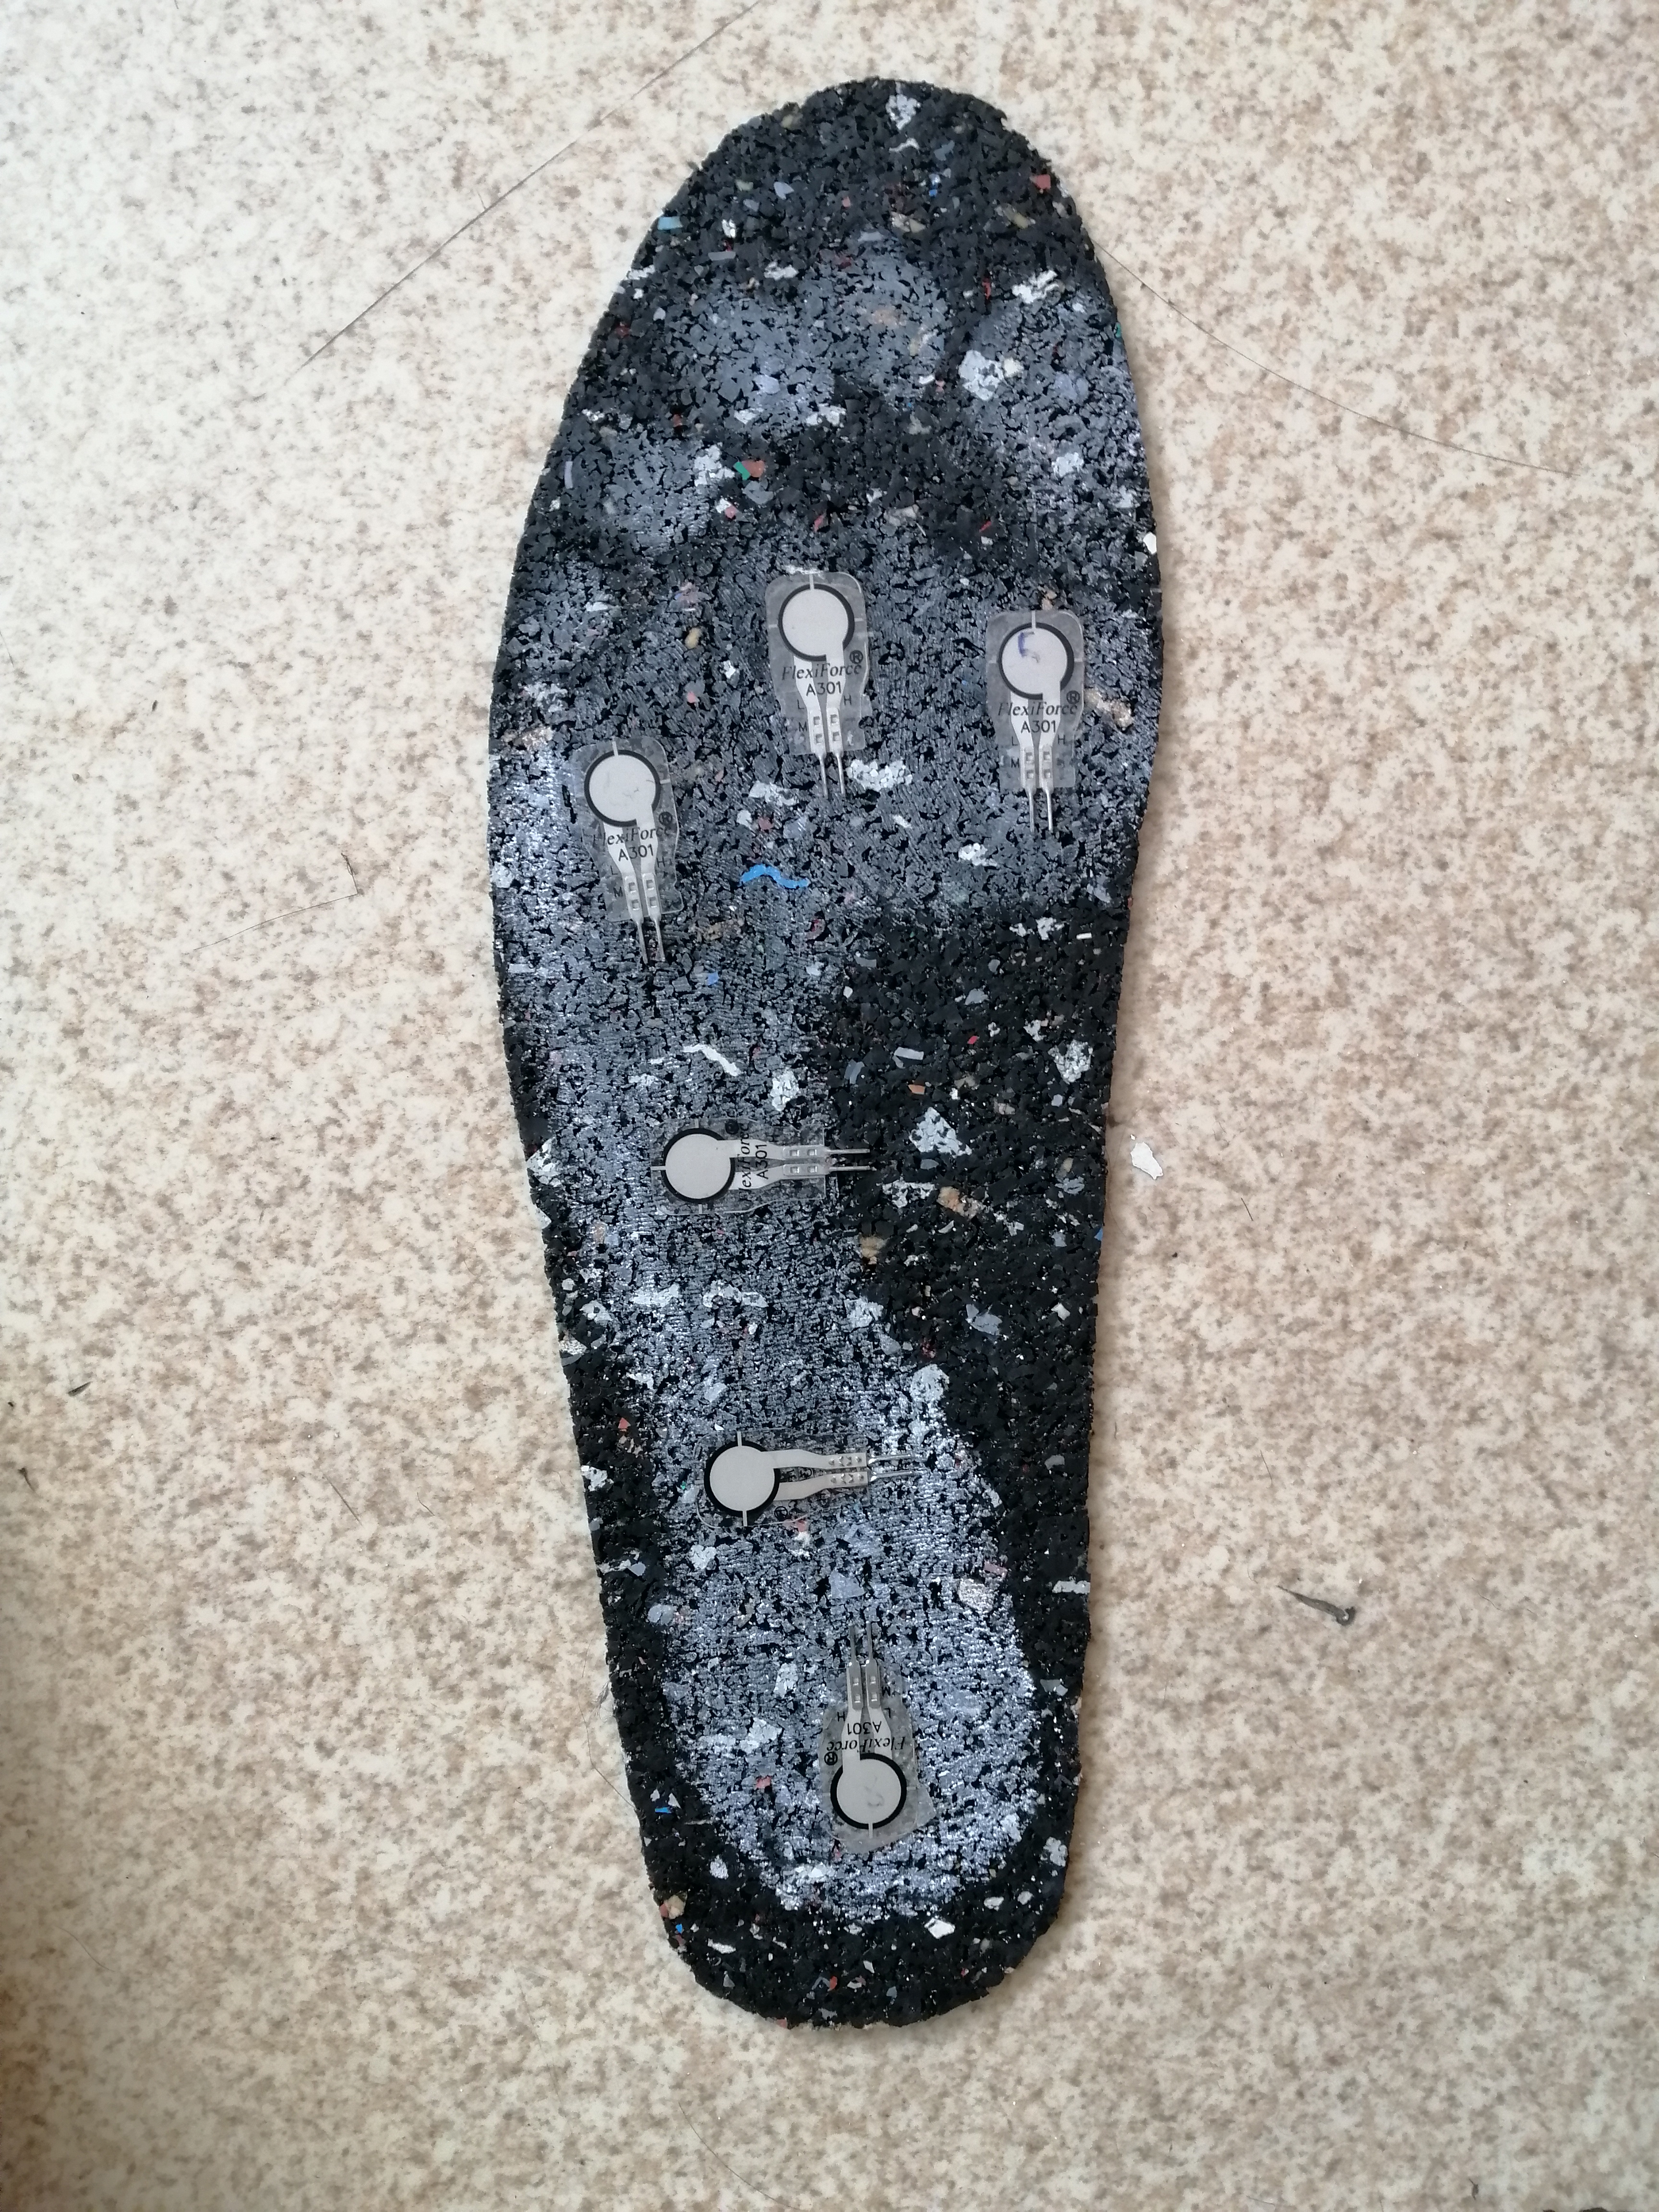
\includegraphics[width=50mm]{sensorPos.jpg}
\hfill
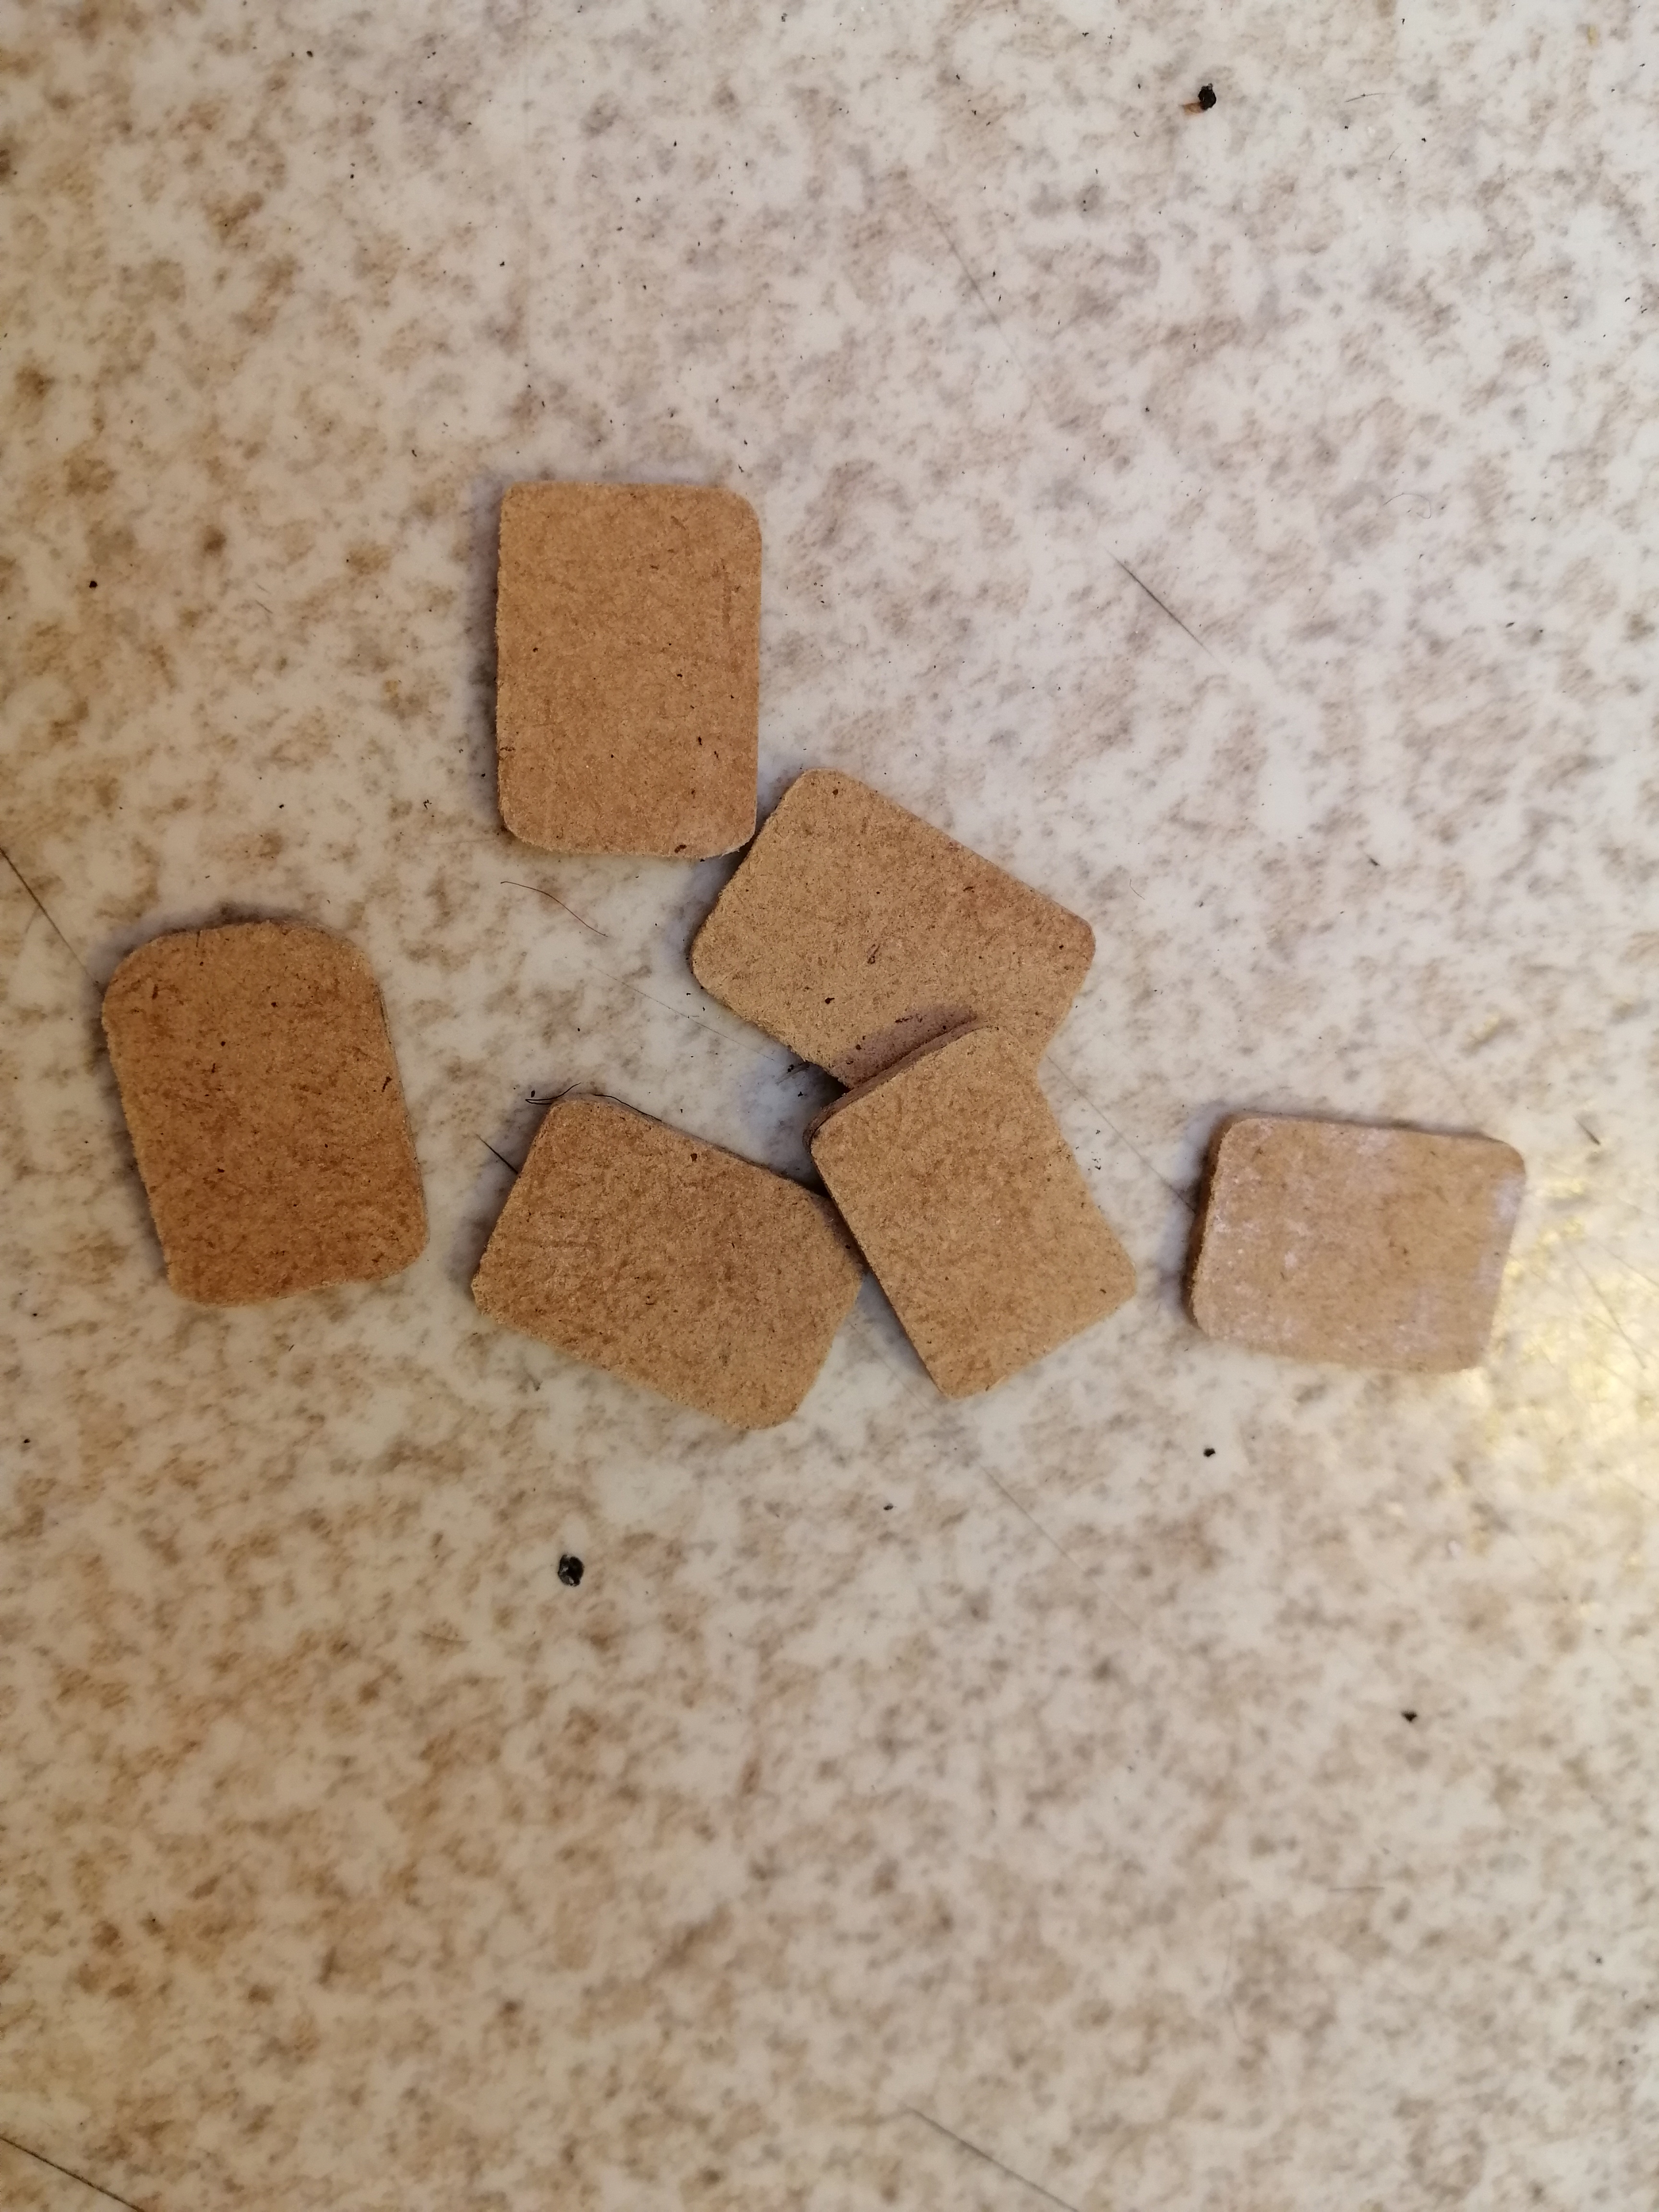
\includegraphics[width=50mm]{pad.jpg}
\end{center}
\end{figure}
% - - - - - - - - - - - - - - - - - - - - - - - - - - - - - - - - - - - 
For the mounting of the insole, because the rubber possess vertical elasticity, it could also damage the sensor in operation. In order to prevent this, the mounting area of the sensors were installed with wood. Instants of small wood pads with the dimension of the sensors were made using a hand saw and a electronic hand screw. These are then put into the insole by using hot glue.\\
\begin{figure}[hbt!]
\begin{center}
\includegraphics[width=50mm]{padPos.jpg}
\hfill
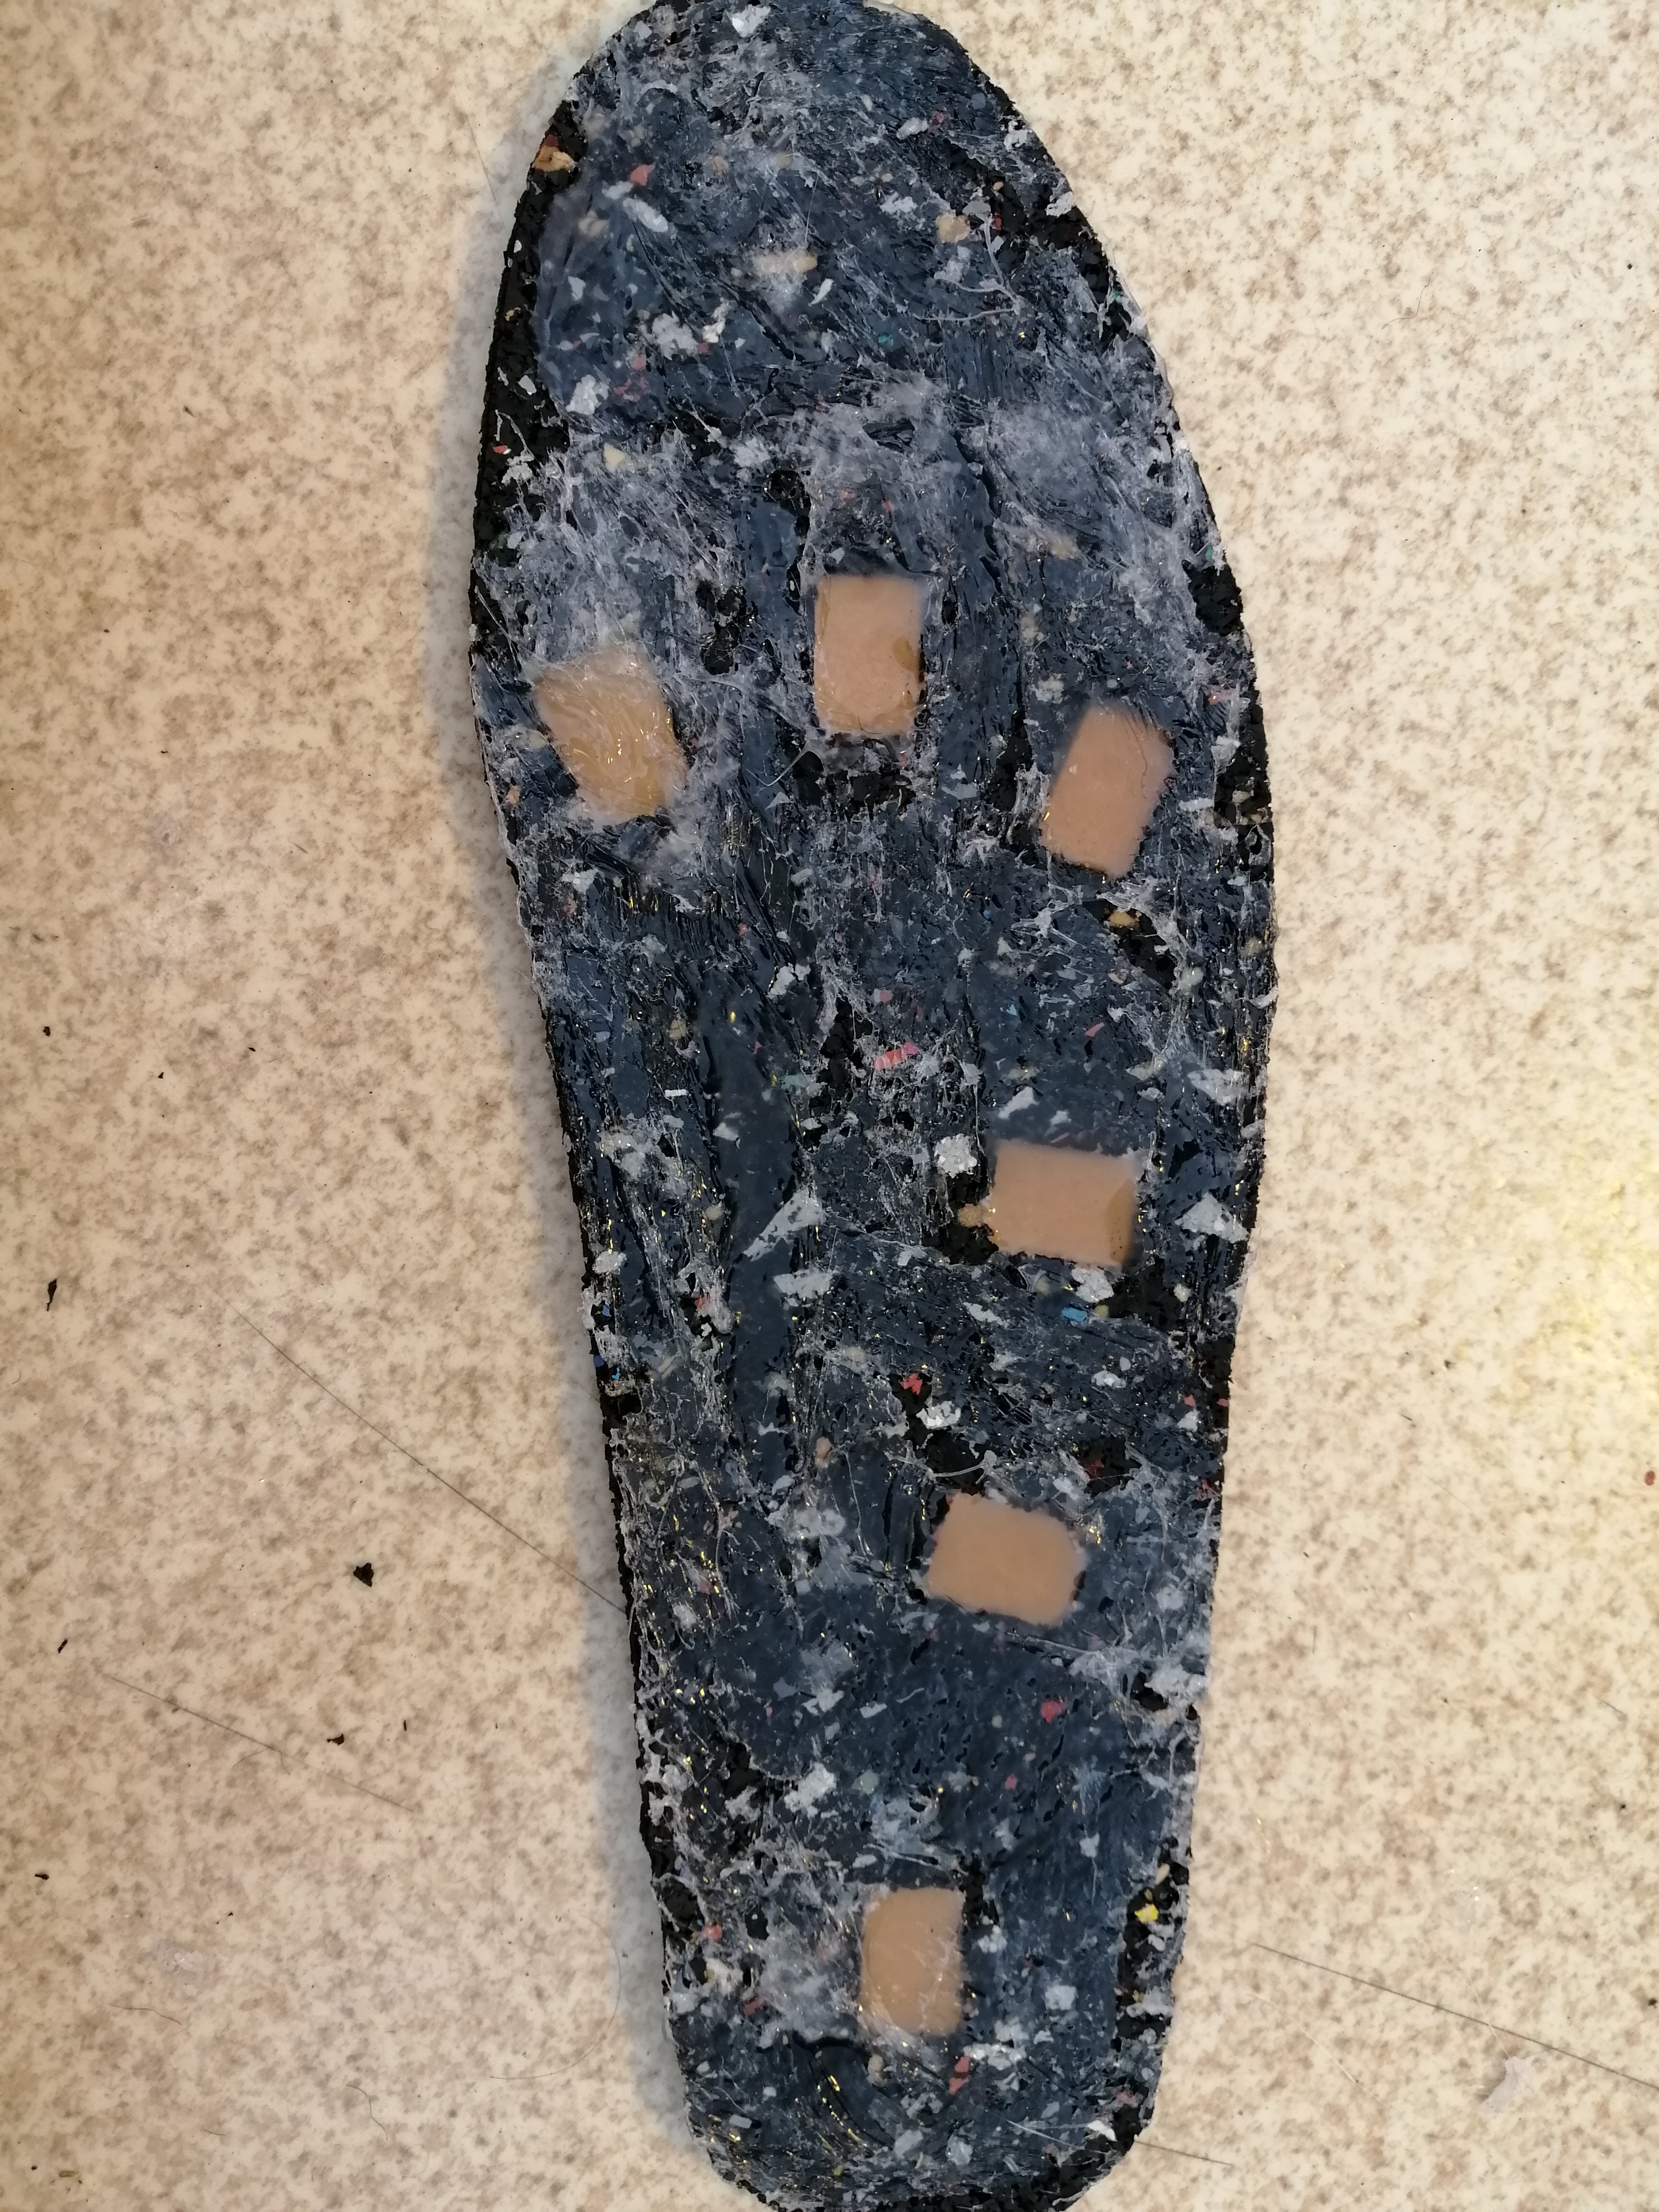
\includegraphics[width=50mm]{padGlue.jpg}
\hfill
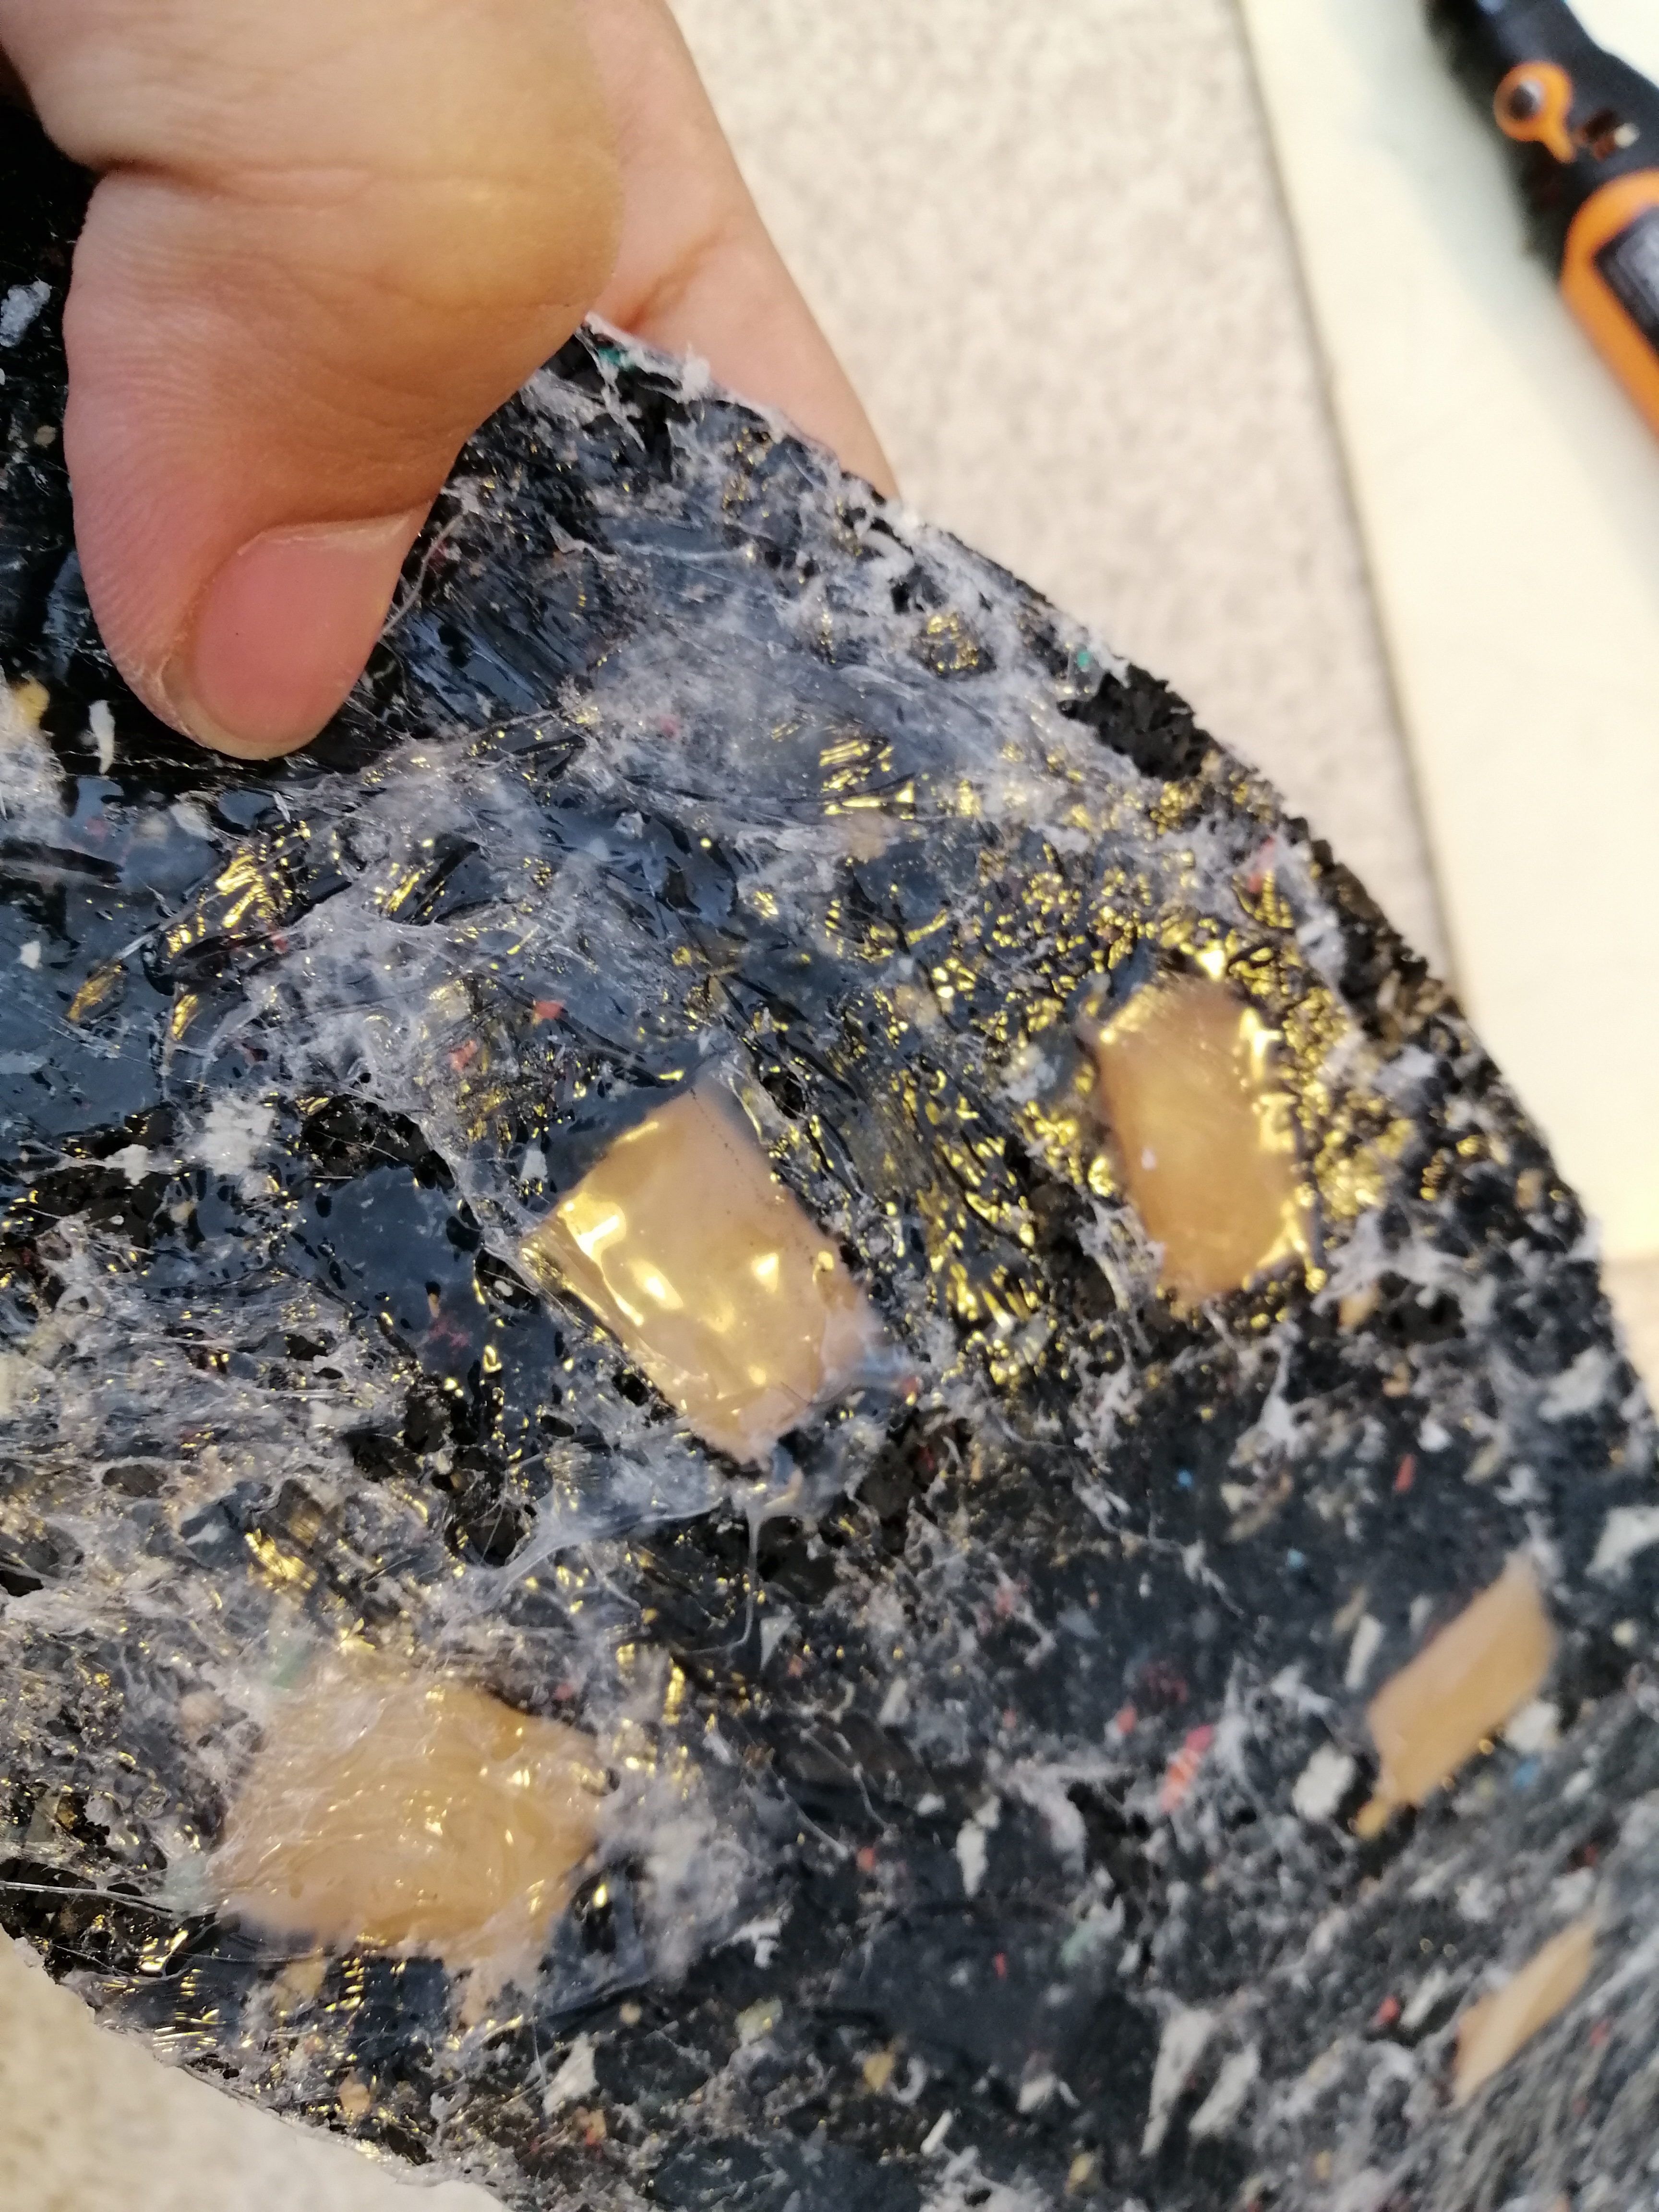
\includegraphics[width=50mm]{padGlueClose.jpg}
\end{center}
\end{figure}
after letting the glue condense, a paper knife was used to trimmed the abundant glue. This help keep the insole thin enough. Then the Sensors were installed onto the wood pad with rubber tape, followed by 2 female pinhead wires. The surroundings of the tape were then glued again, to secure it from falling off.\\
\begin{figure}[hbt!]
\begin{center}
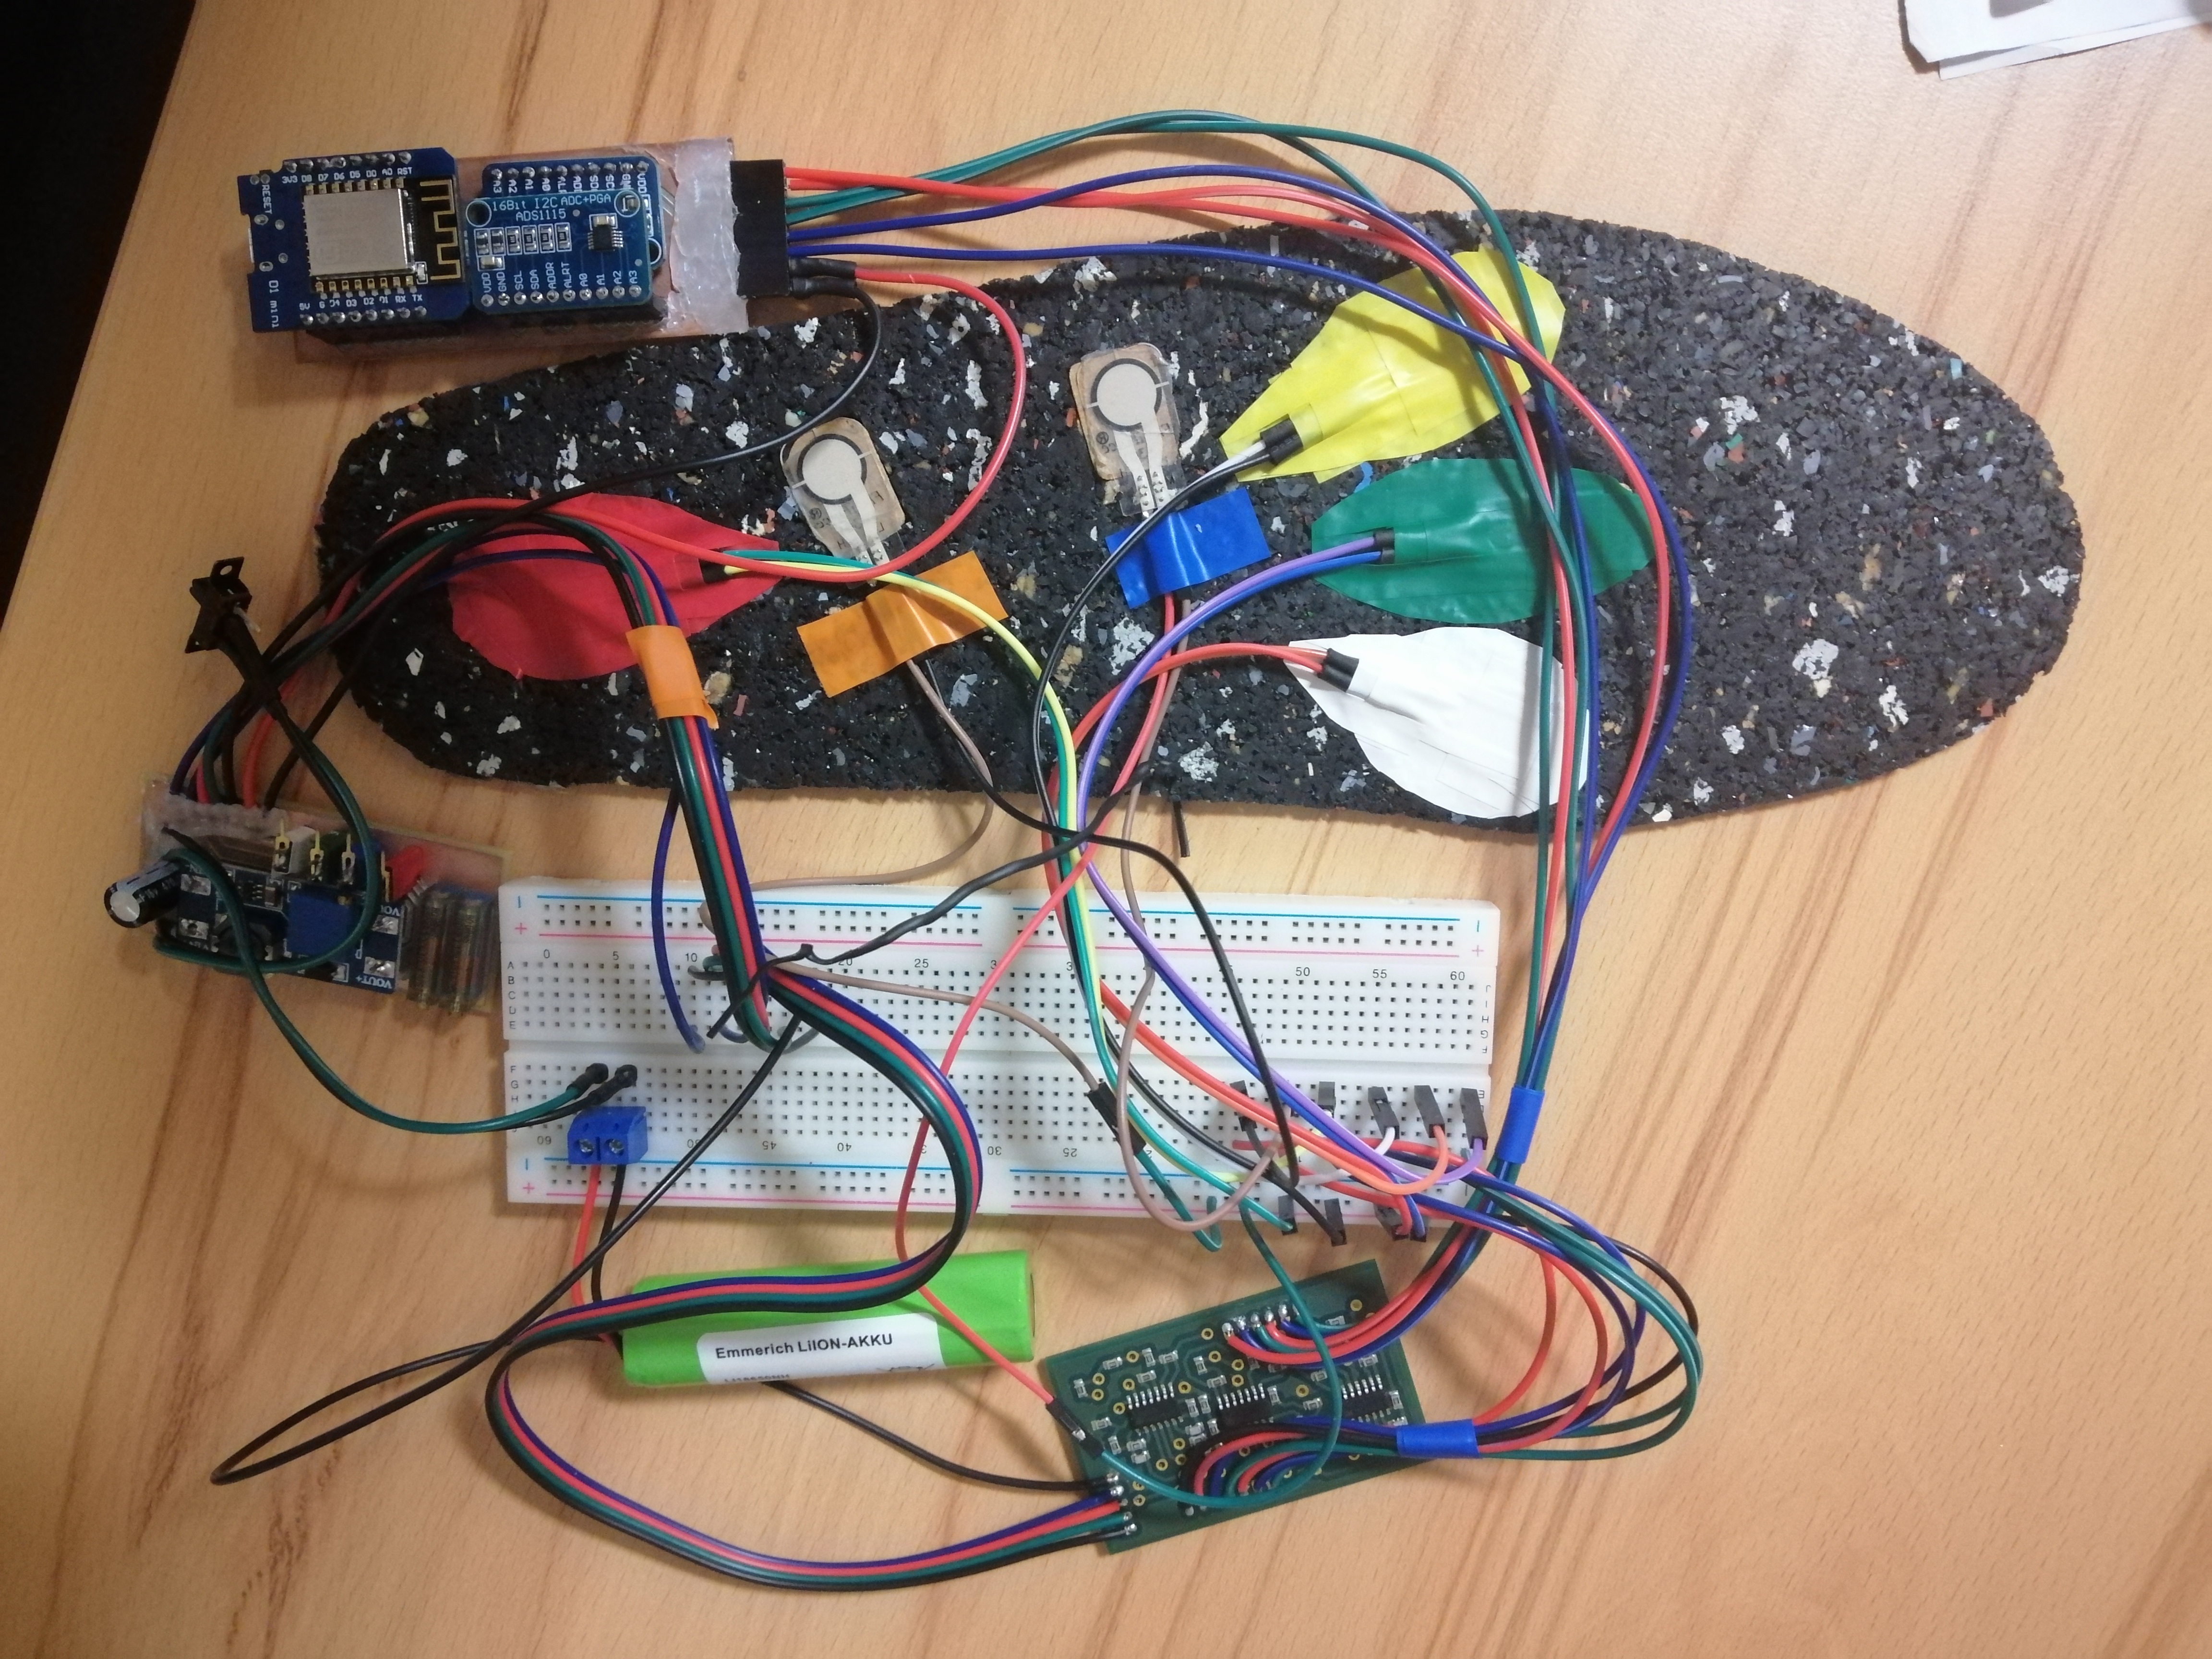
\includegraphics[width=150mm]{completeProt.jpg}
\caption{Complete prototype before casing and mounting on shoe}
\end{center}
\end{figure}
The wiring of the sensors was made that every sensors has one end connected to VG/2 and the other end as output signal from sensor. For intuition they can be called impedance output. these outputs were then fed into the Force Board, for signal conditioning. The interface between the insole and the force board are 7 lines - 6 impedance output + 1 VG/2.
% - - - - - - - - - - - - - - - - - - - - - - - - - - - - - - - - - - - 
\subsection{shoe installment}
After the breadboard test, the insole was tested for durability in the specified shoe. It was put inside under the shoe's original insole, with no wiring and boards connected. Normal movement include running, walking climbing stairs to see if the durability is satisfied.\\
After that, the whole system was put on the test to see the connection through Wifi and the signal conditioning board operation. Some errors were detected and dealt with during the recheck, see Discussion. \\
\begin{figure}[hbt!]
\centering
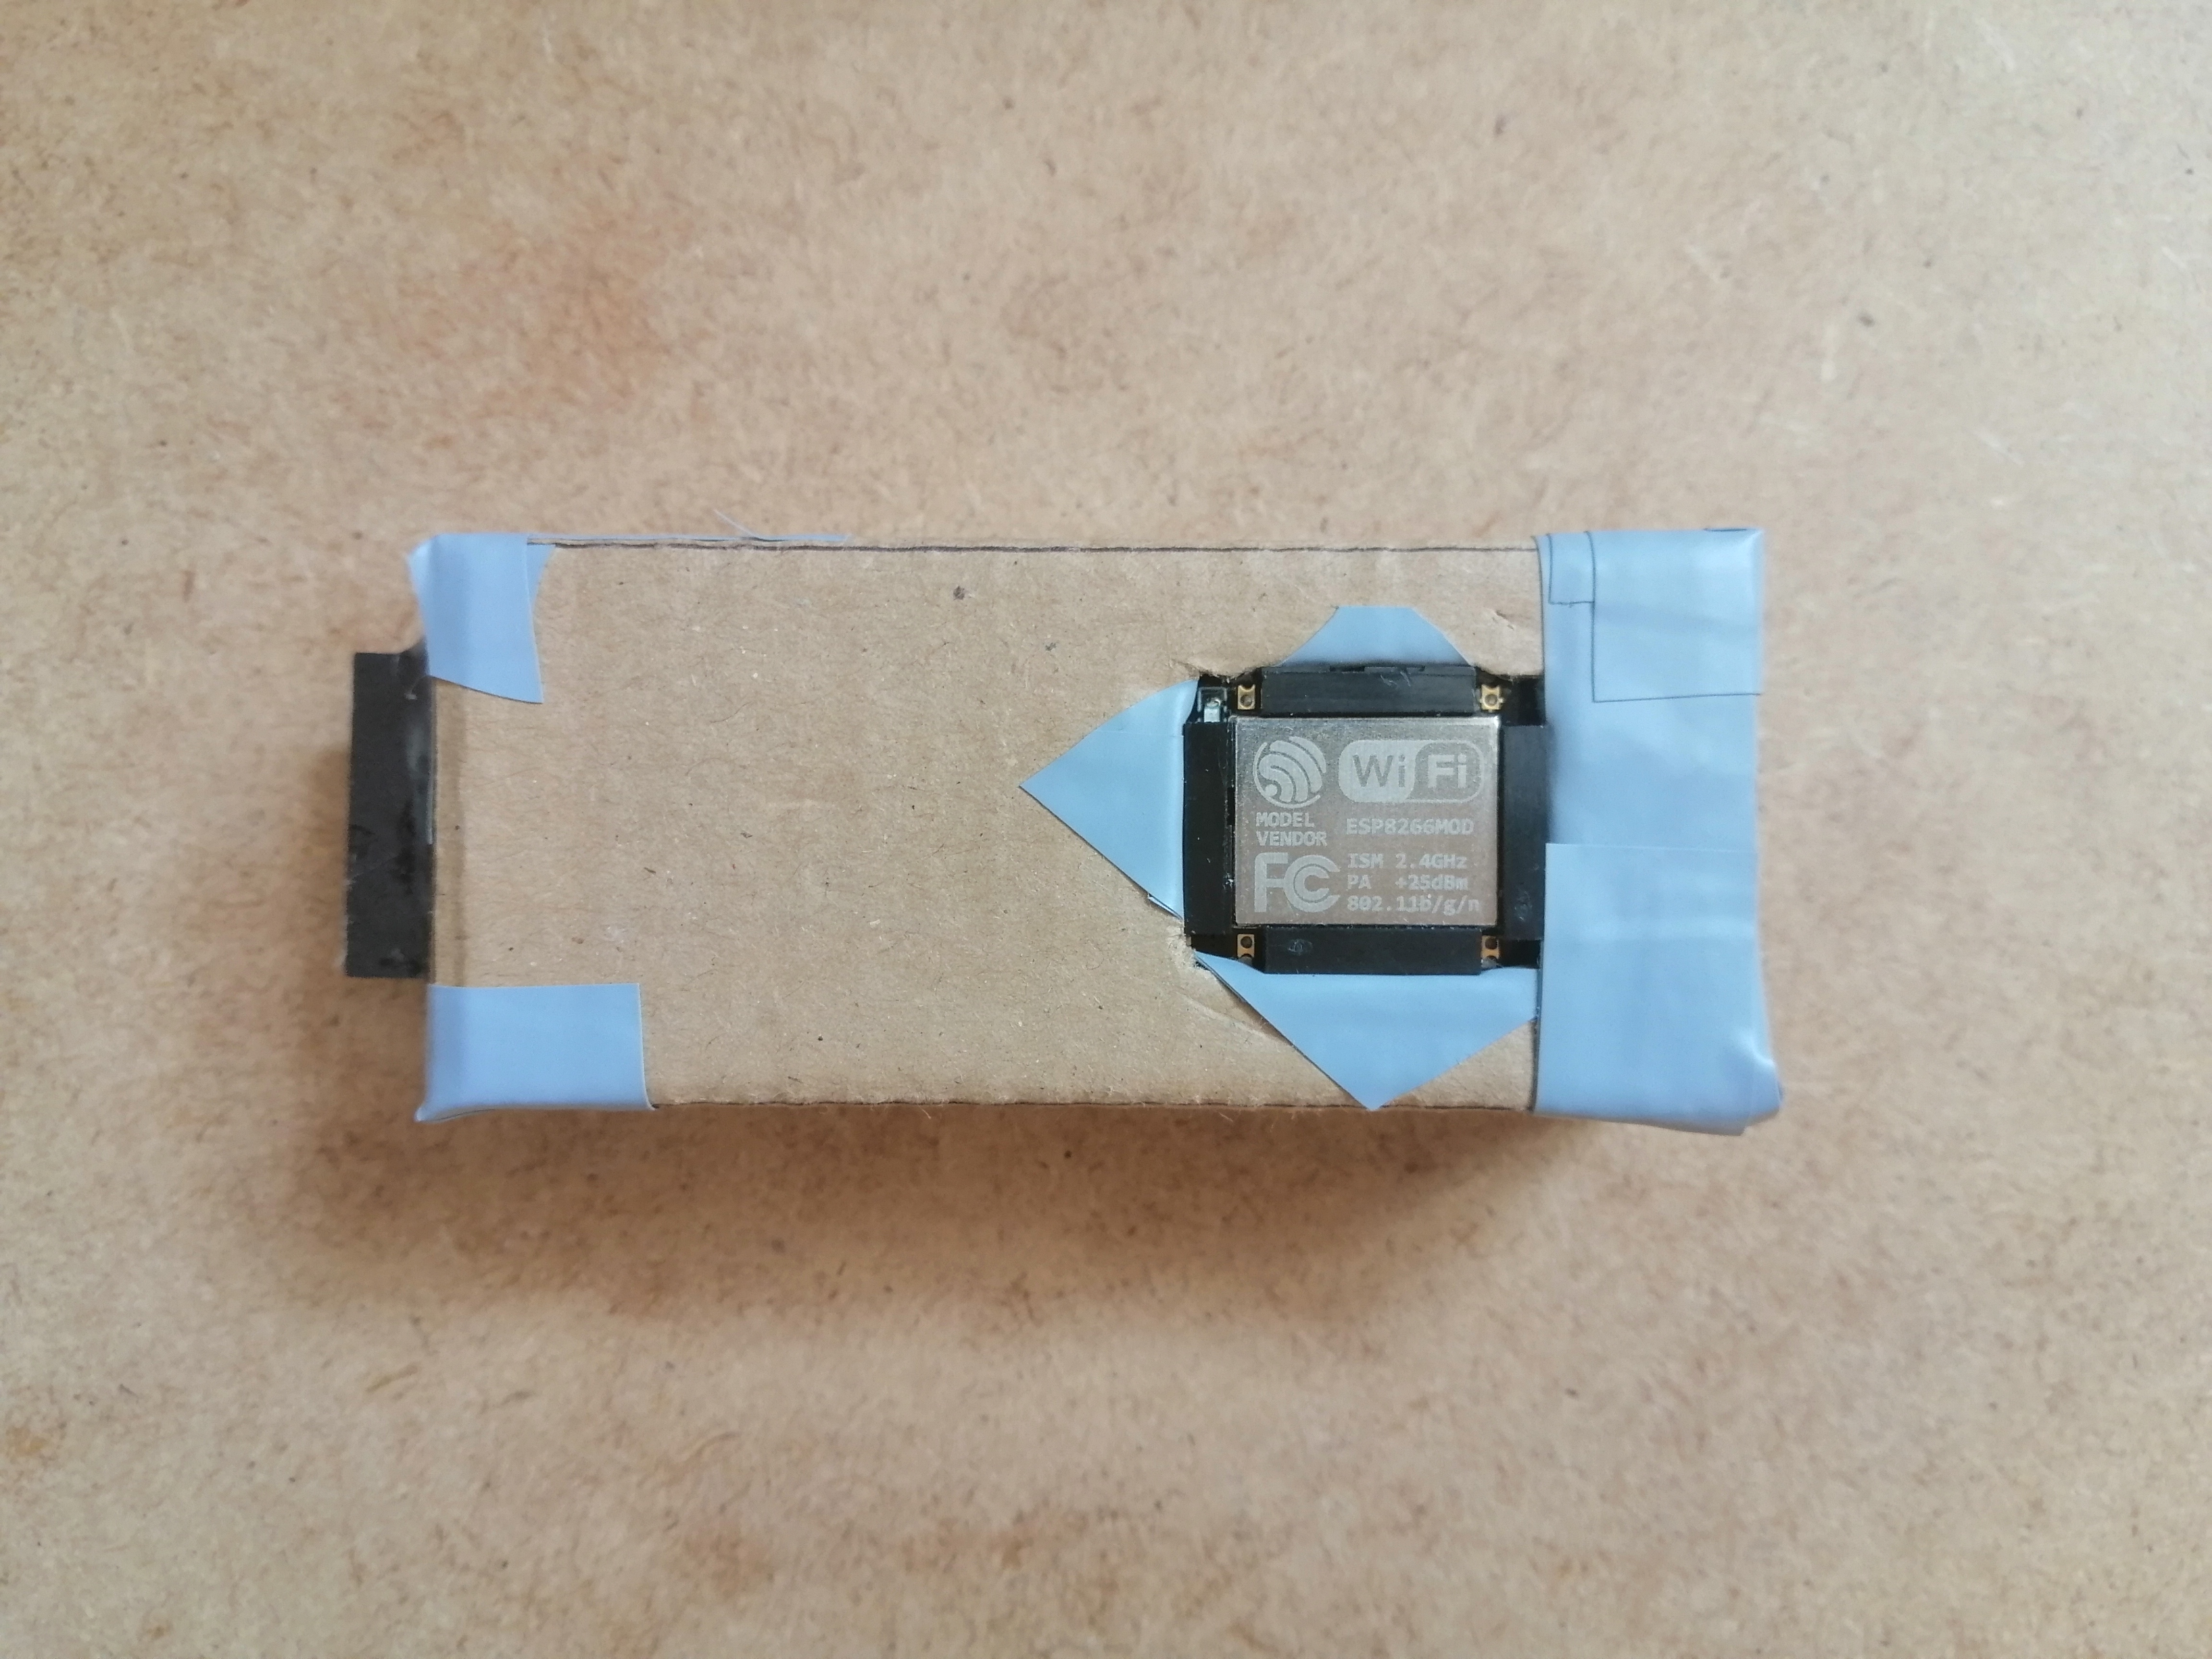
\includegraphics[width=50mm]{DataBoardCased.jpg}
\hfill
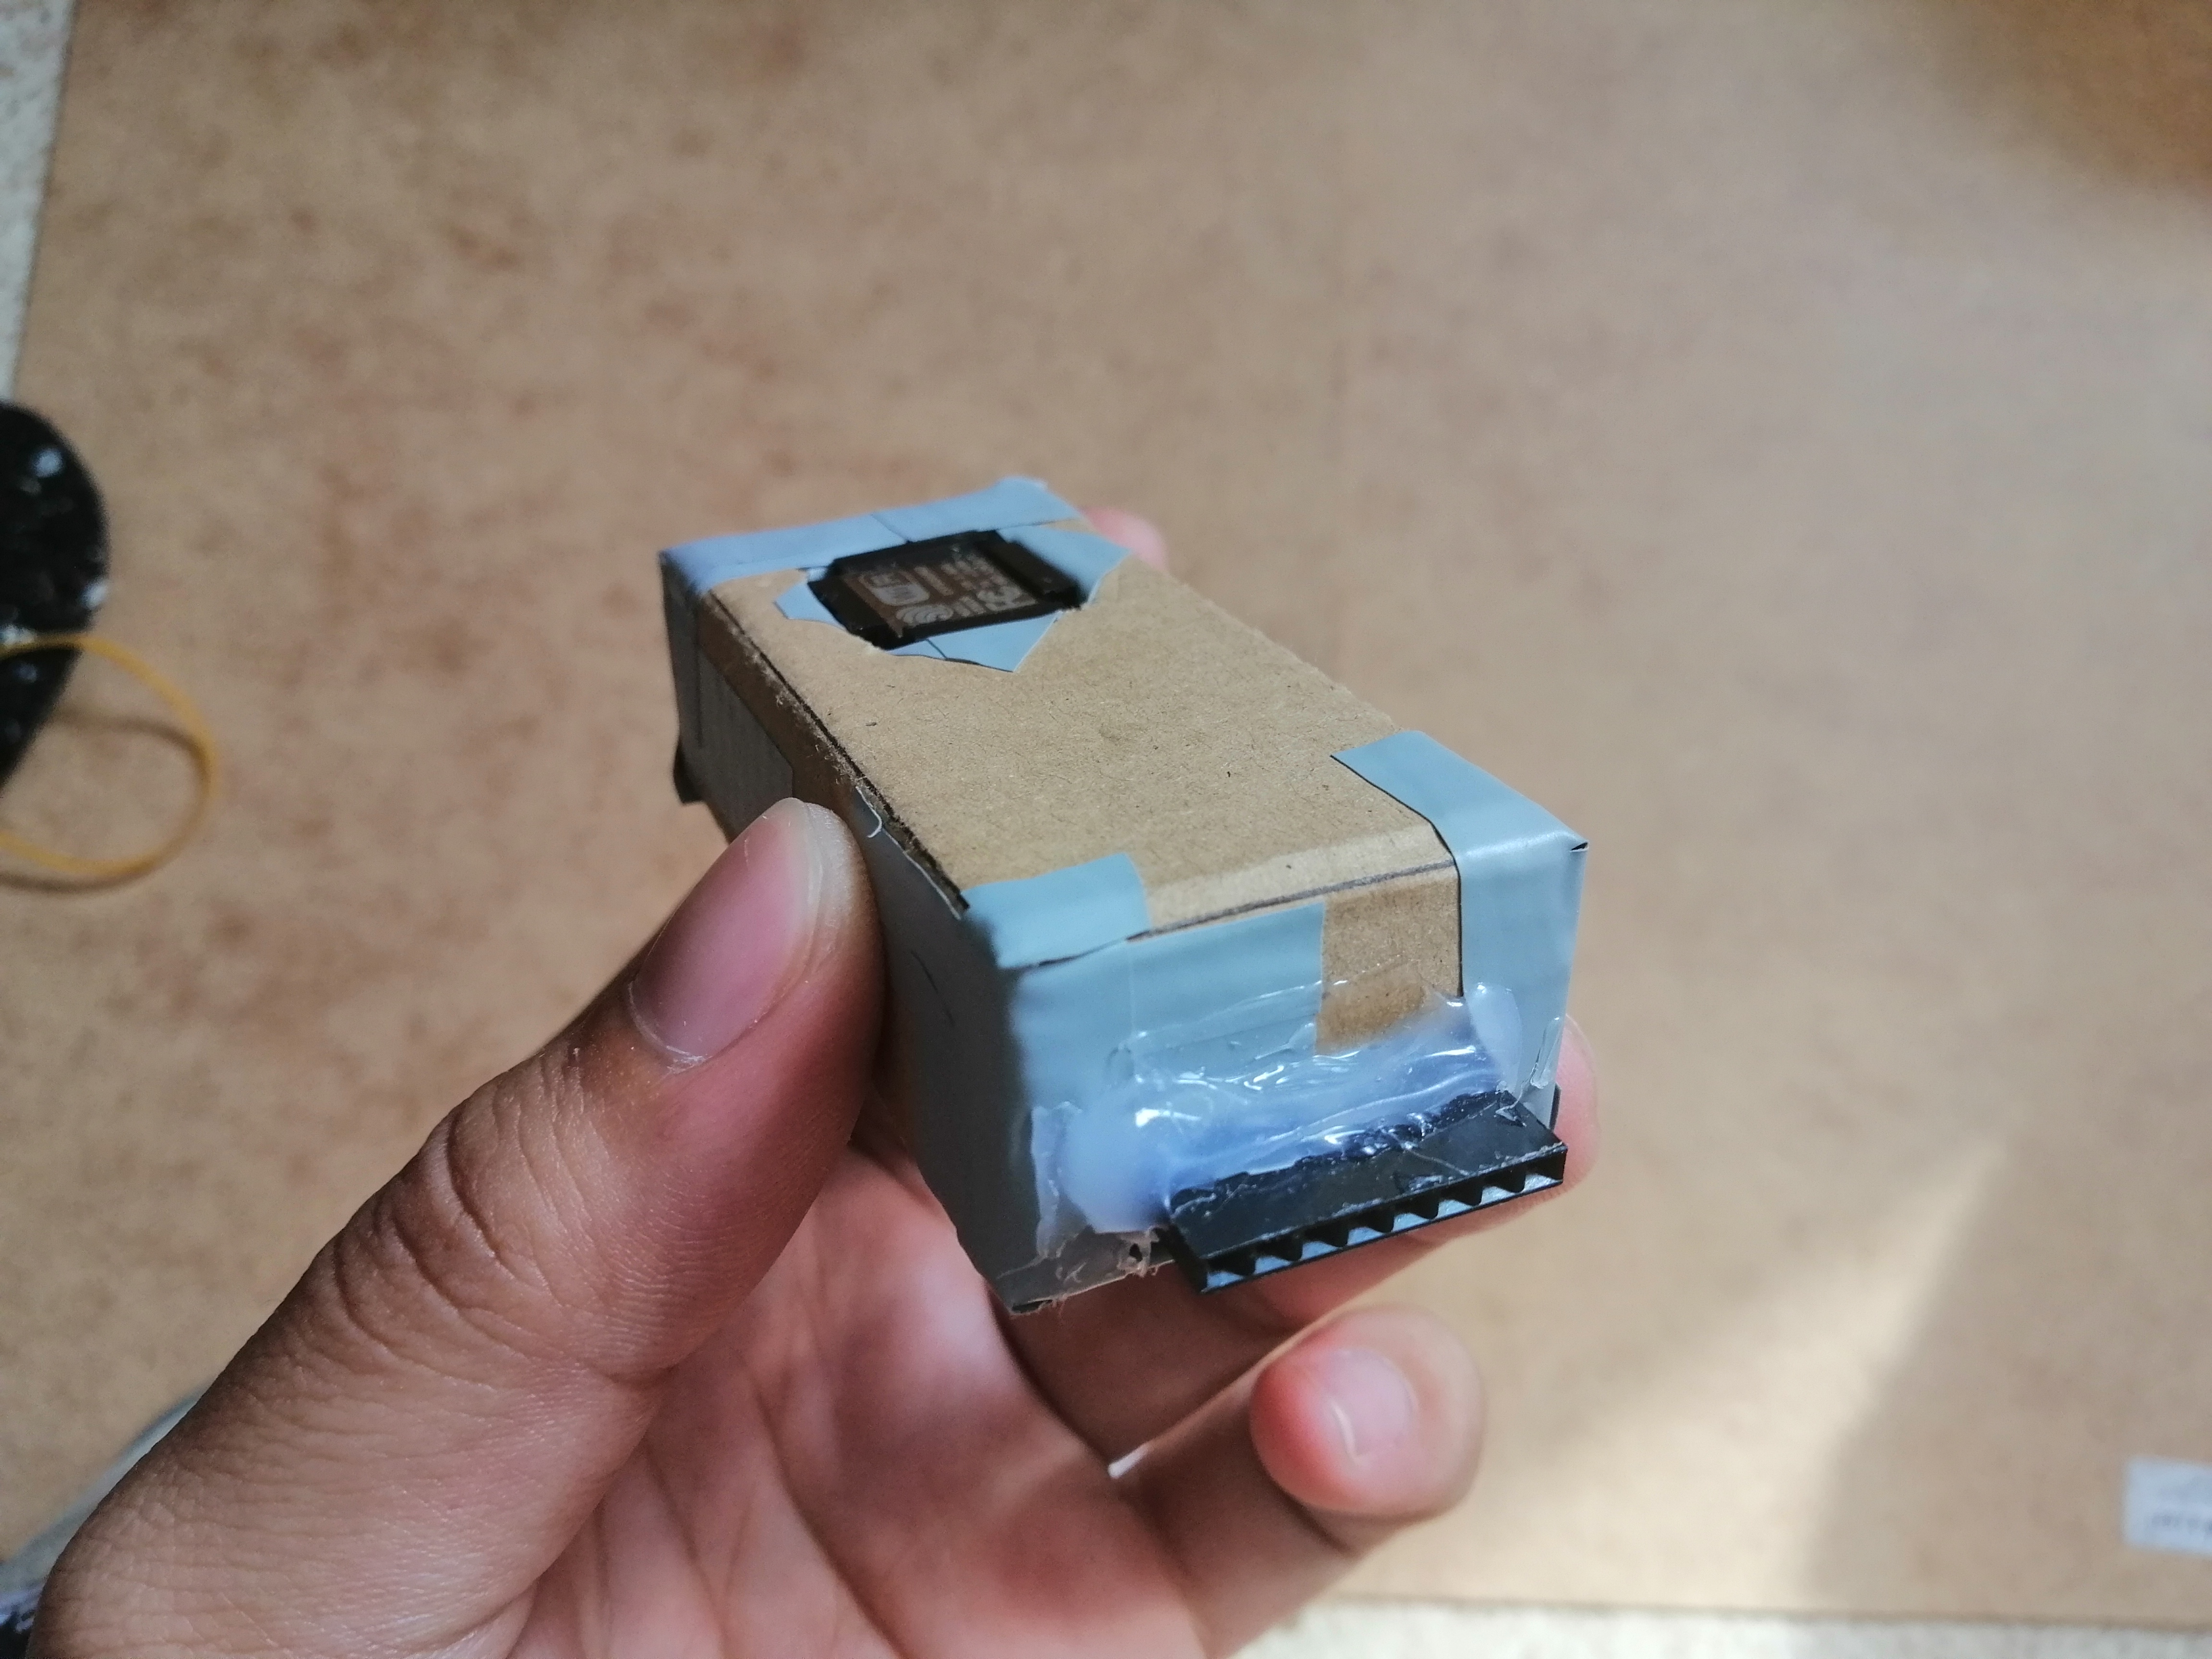
\includegraphics[width=50mm]{DataBoardInterface.jpg}
\hfill
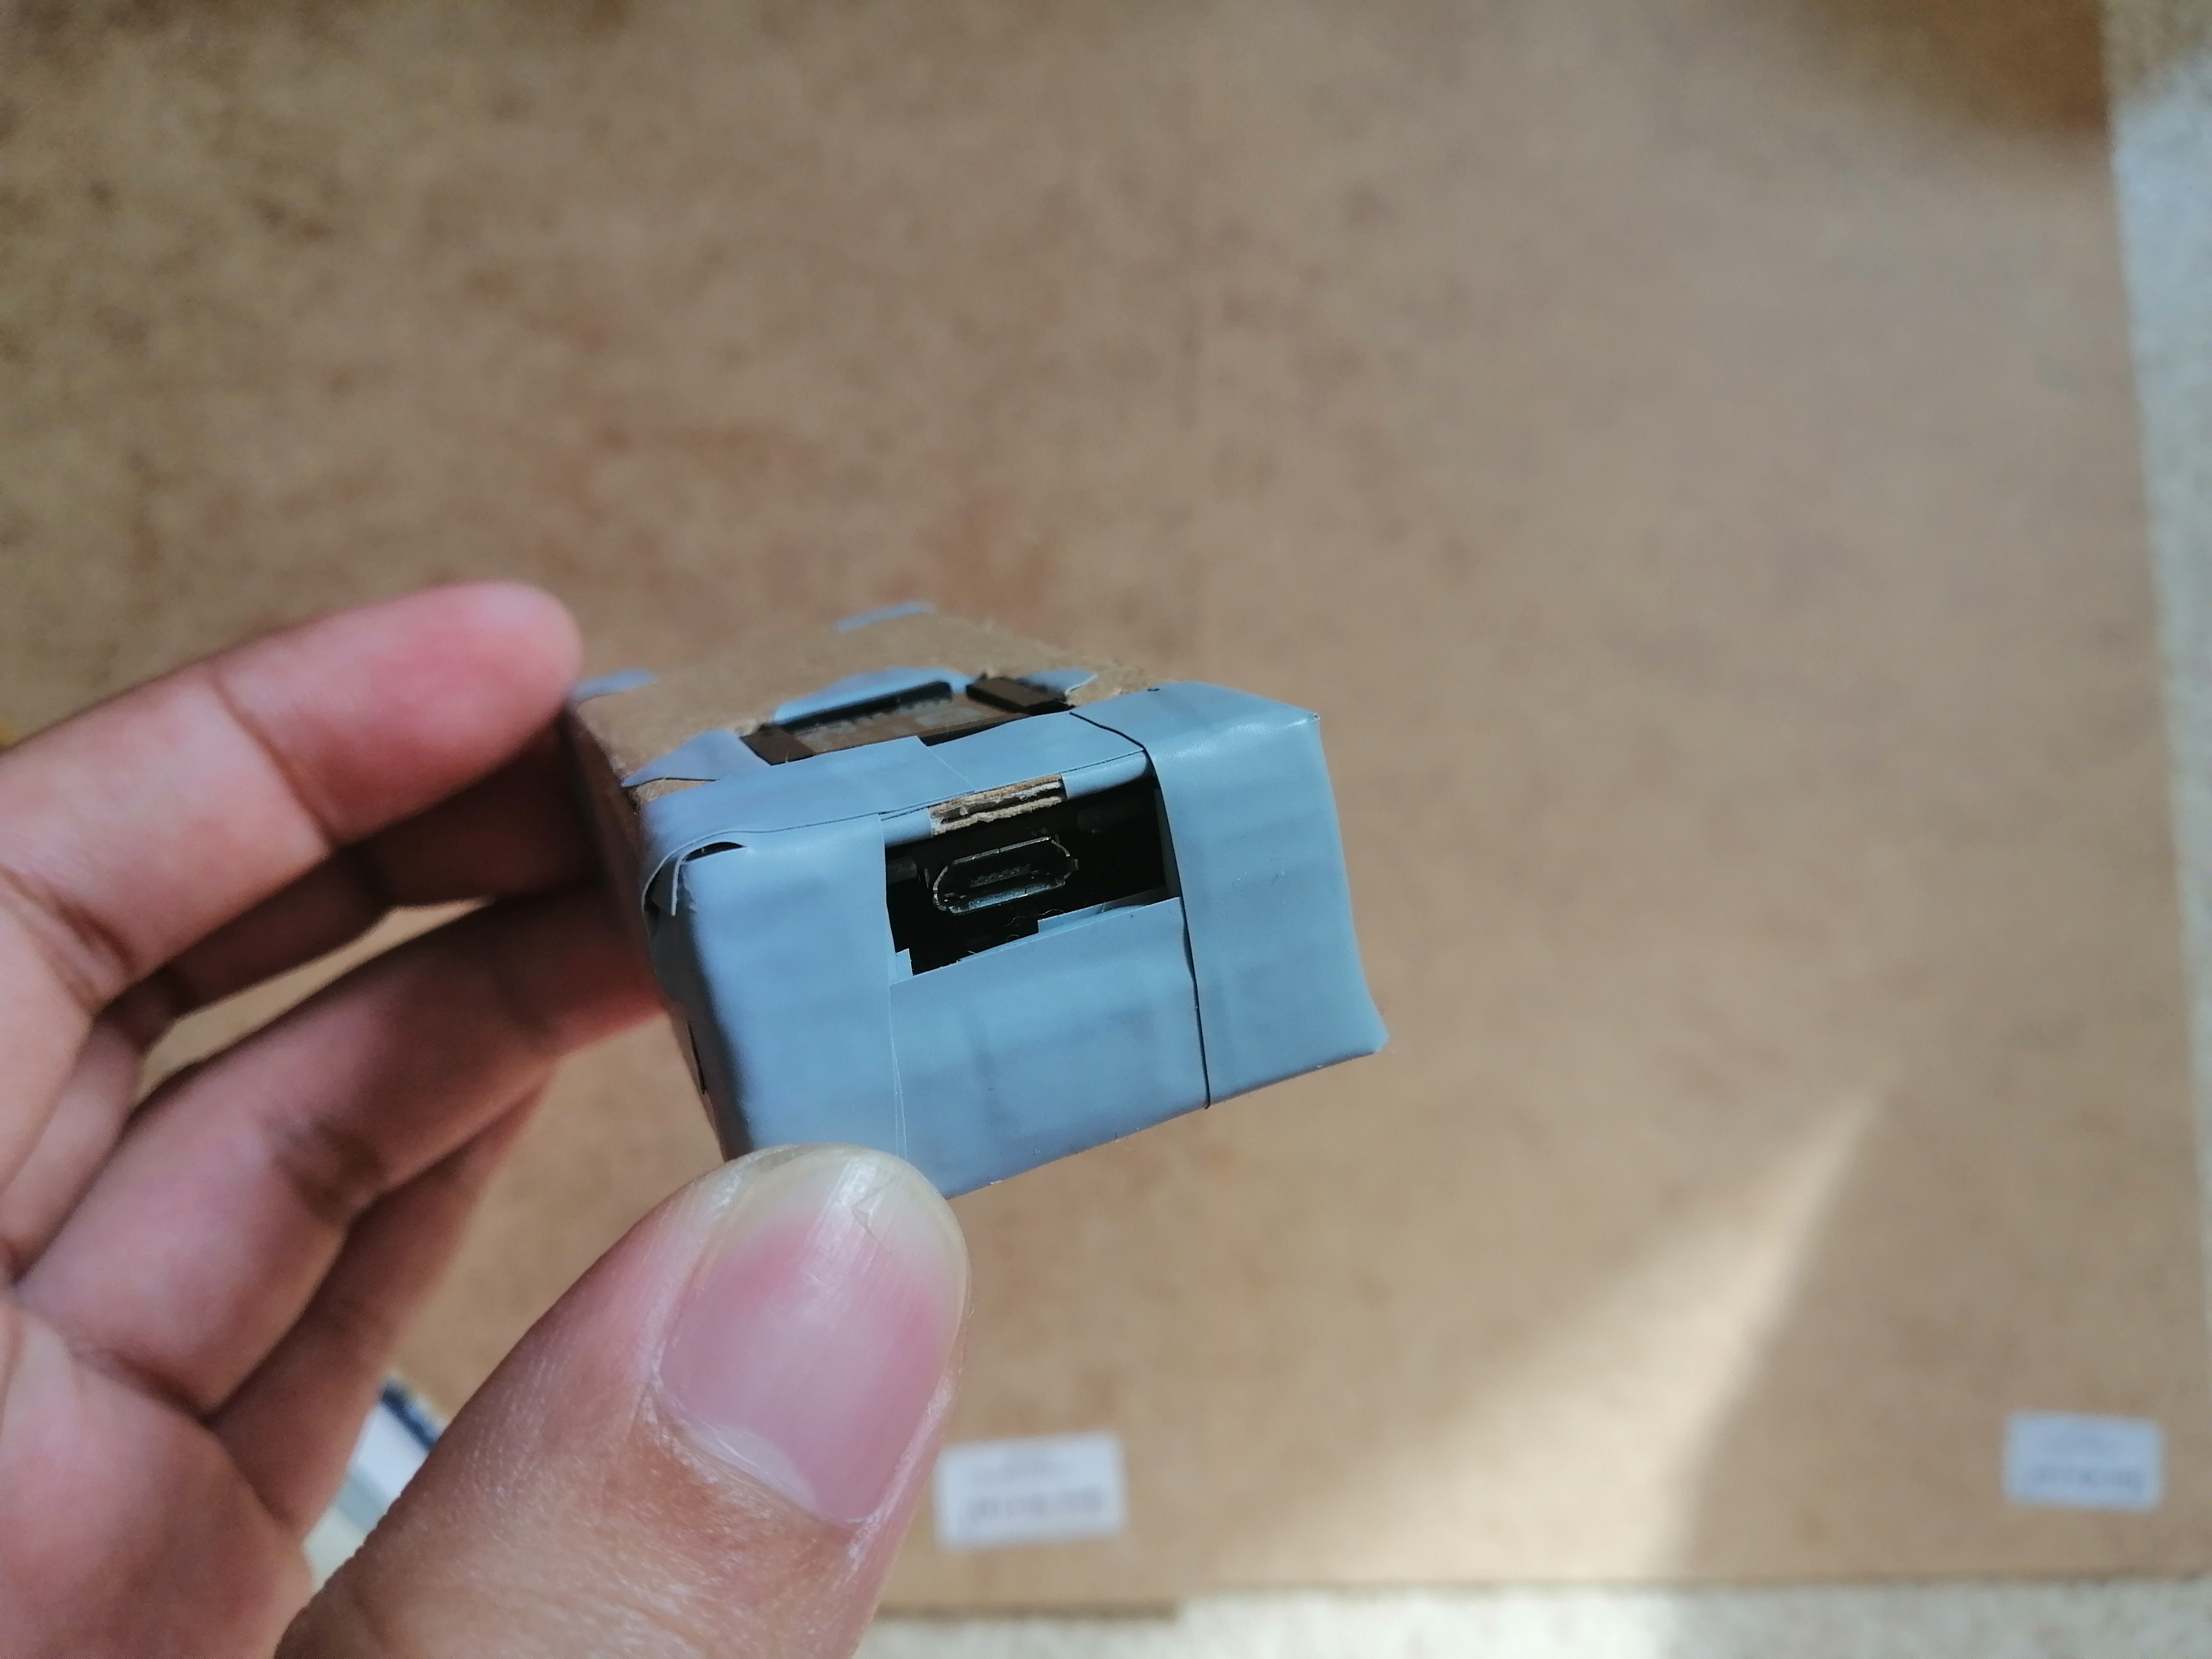
\includegraphics[width = 50mm]{DataBoardMicro.jpg}
\caption{Data Board after casing}
\end{figure}
After fixing the errors the shoe is put into casing. Current casing used carton box. The Carton blueprints were cut in the dimension of the boards and then stitched together with electrical tape. The inside of the carton boxes were also insulated by covering them with electrical tape. This was to put some insulation to the electrical boards inside, as by all means carton become a conductor when it get wet. It would have been preferable to use plastic, or mica casing. But there weren't enough time for these better option.\\
\begin{figure}[hbt!]
\centering
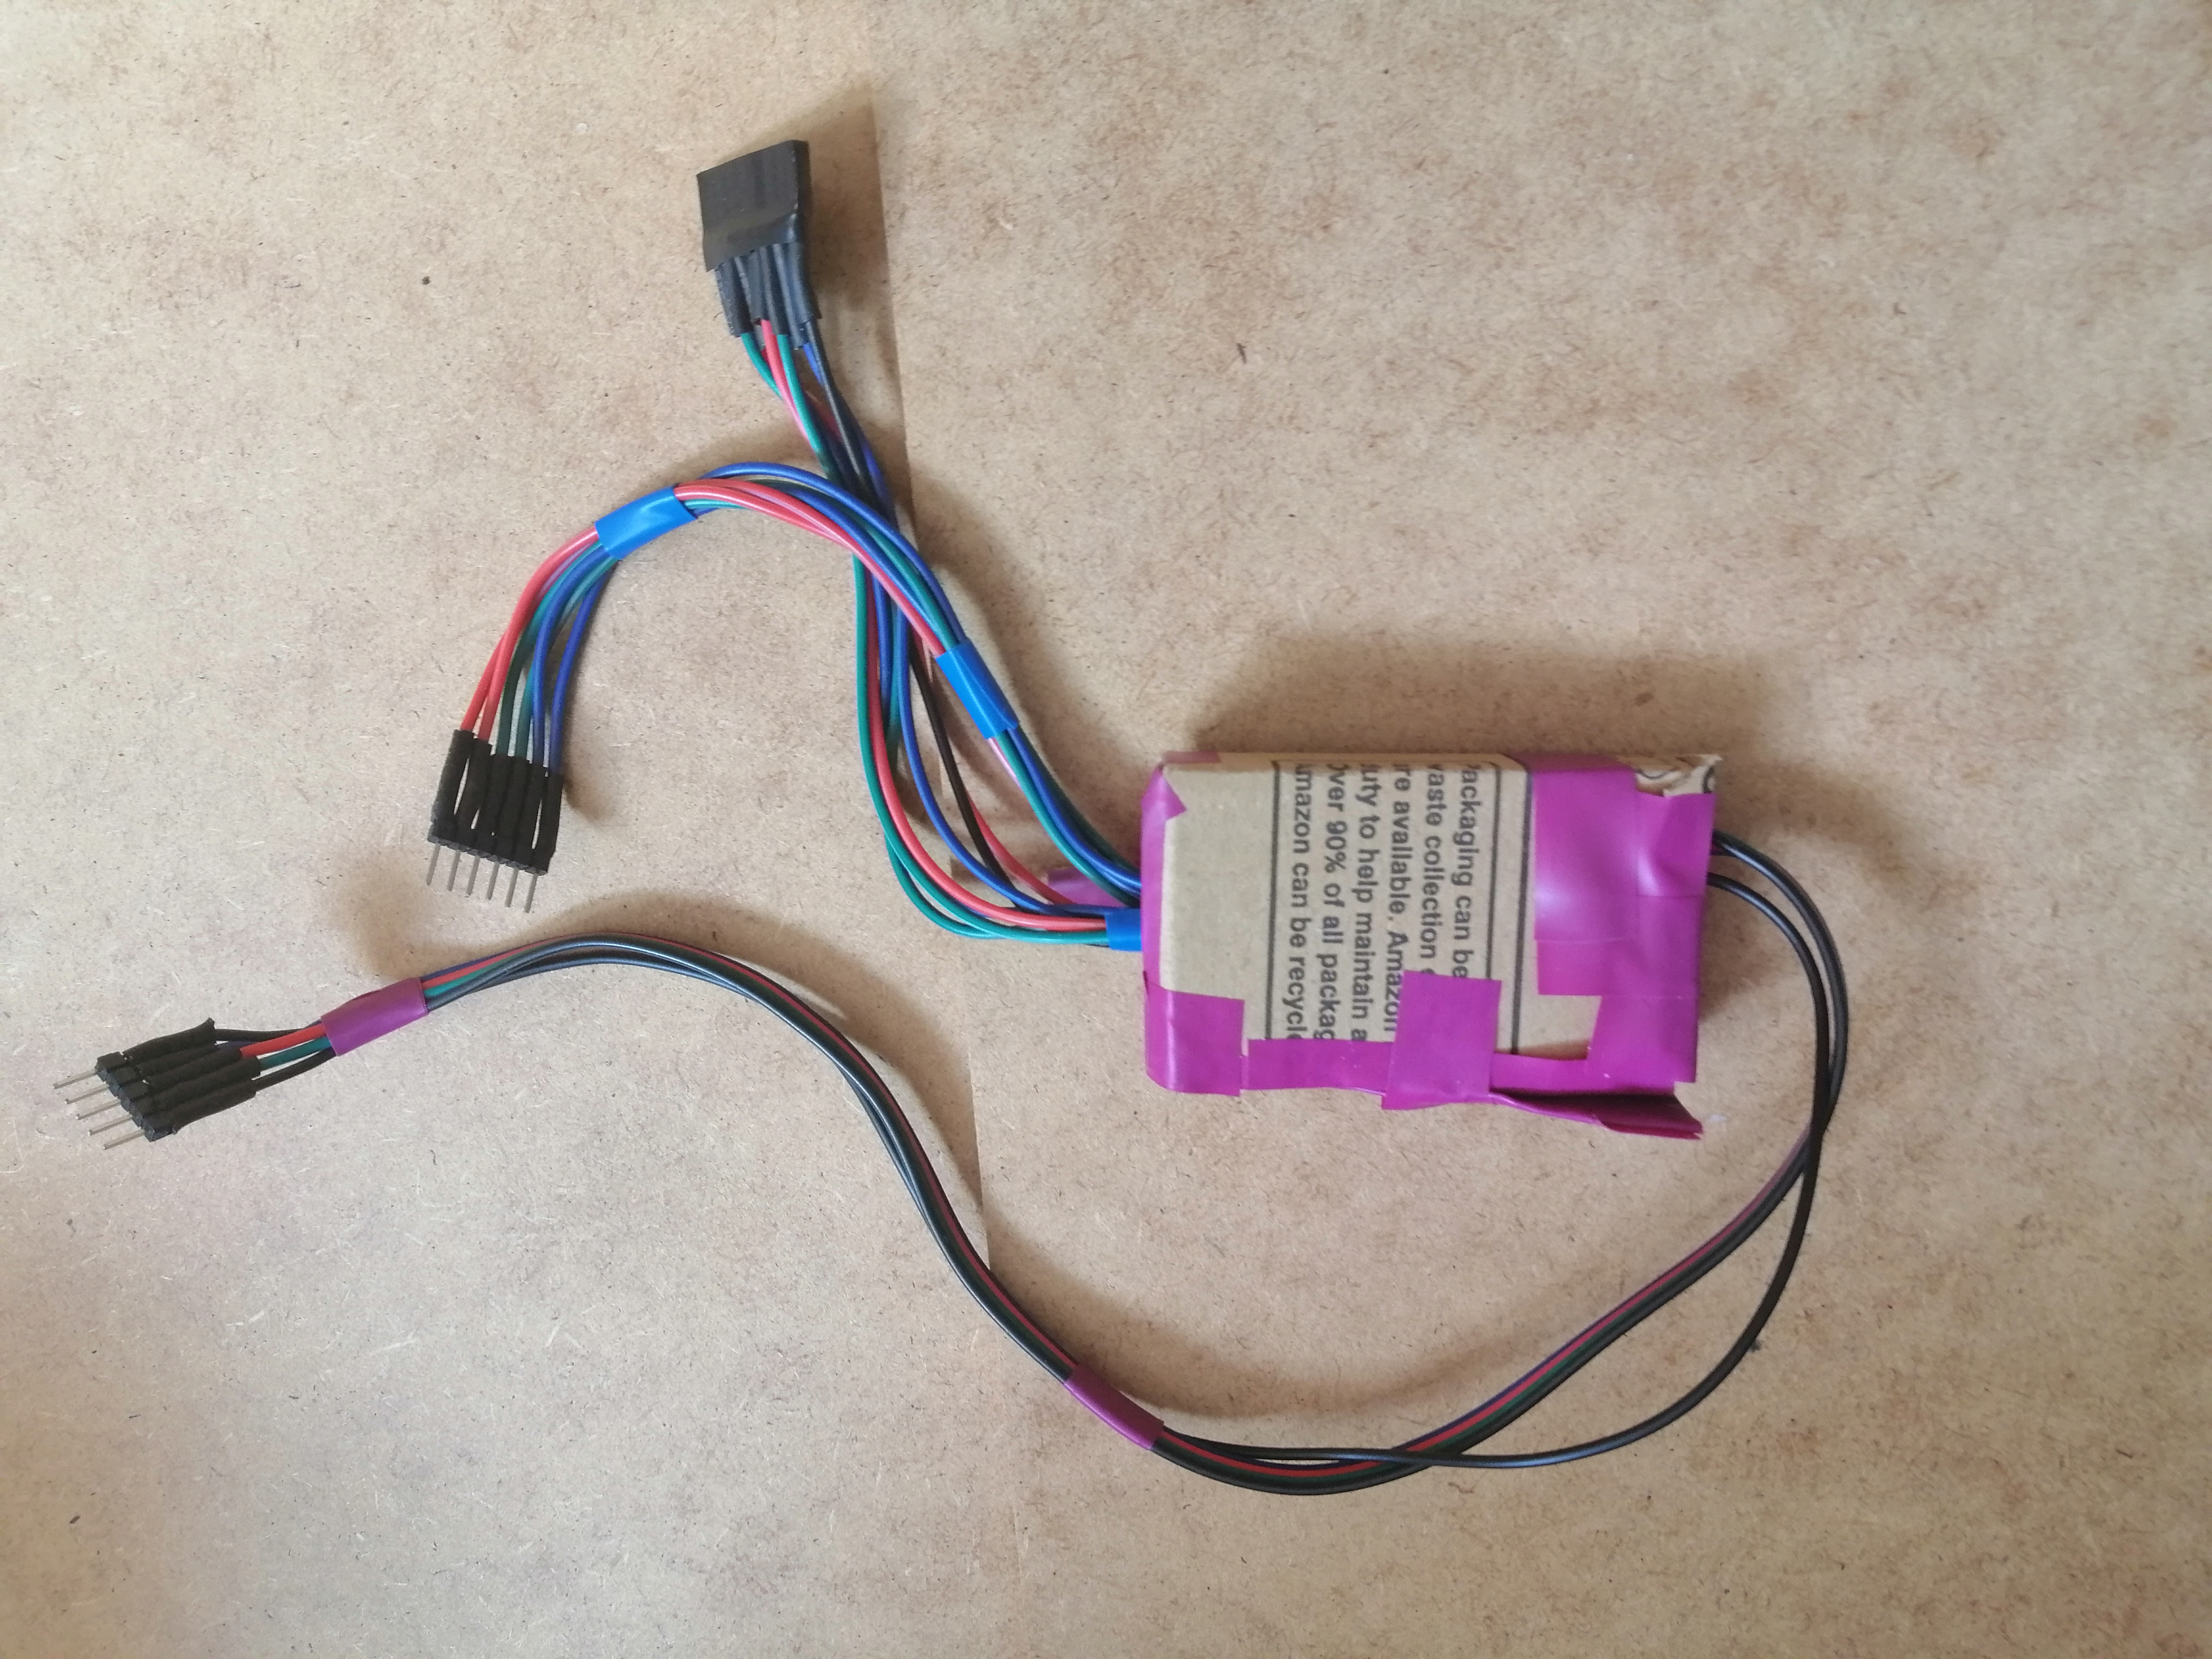
\includegraphics[width=100mm]{PowerBoardCased.jpg}
\caption{Force Board after casing}
\end{figure}
\begin{figure}[hbt!]
\centering
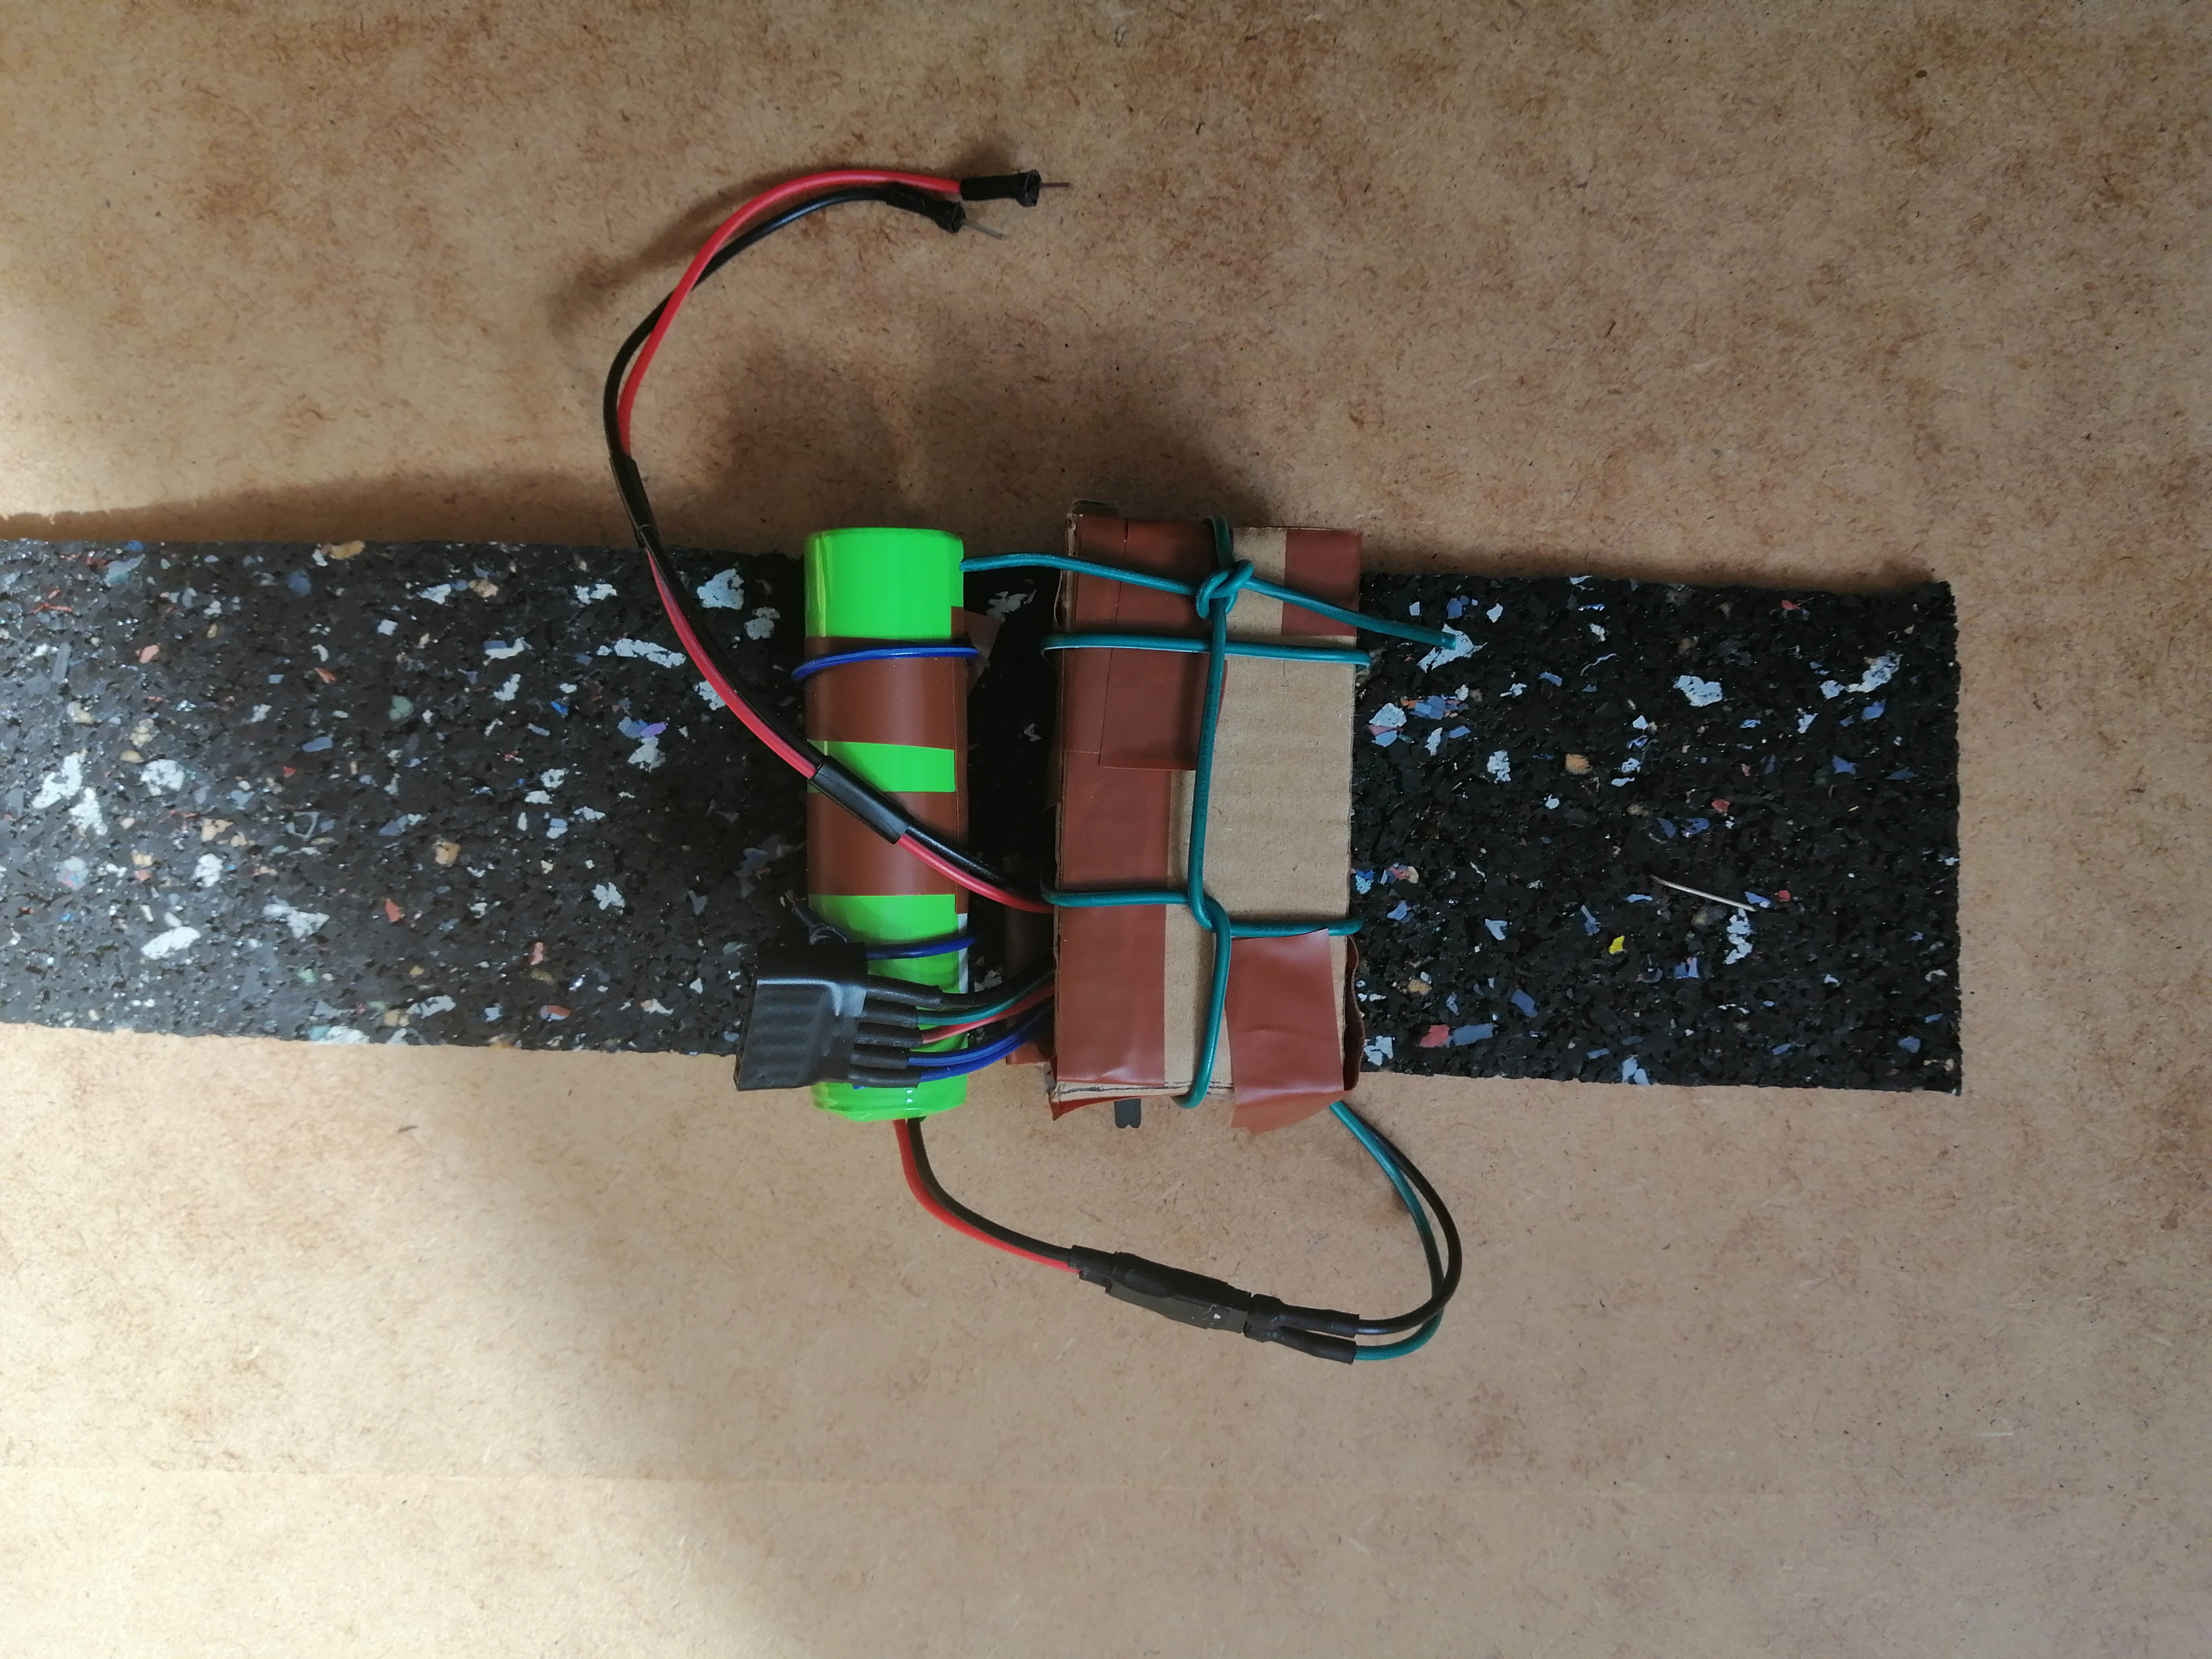
\includegraphics[width = 100mm]{PowerBoard.jpg}
\caption{Power Board after casing and wired on the rubber strap, with 18650 battery}
\end{figure}
After the casing and insulation were done, the system was put to test again to see if any trouble or errors occurred. When everything was satisfied, the boards and the insole were arranged on the shoe for durability test. The arrangement can be seen in figure ... .The battery and the Power Boards were attached to the upper of the ankle by a recycled rubber strap with paper clip as knot. However the rubber surface was too rough for wearing and may cause abnormalities in gait. A clinical bandage was then used between the rubber strap and the skin. This arrangement ensure the safe operating for the wire connection, and interface. Some Design errors also occurred during durability test to the local supermarket and back. After fixing all the errors and tweaking with some final touch, the hardware part was ready for evaluating the software and developing the processing code.
\begin{figure}[hbt!]
\centering
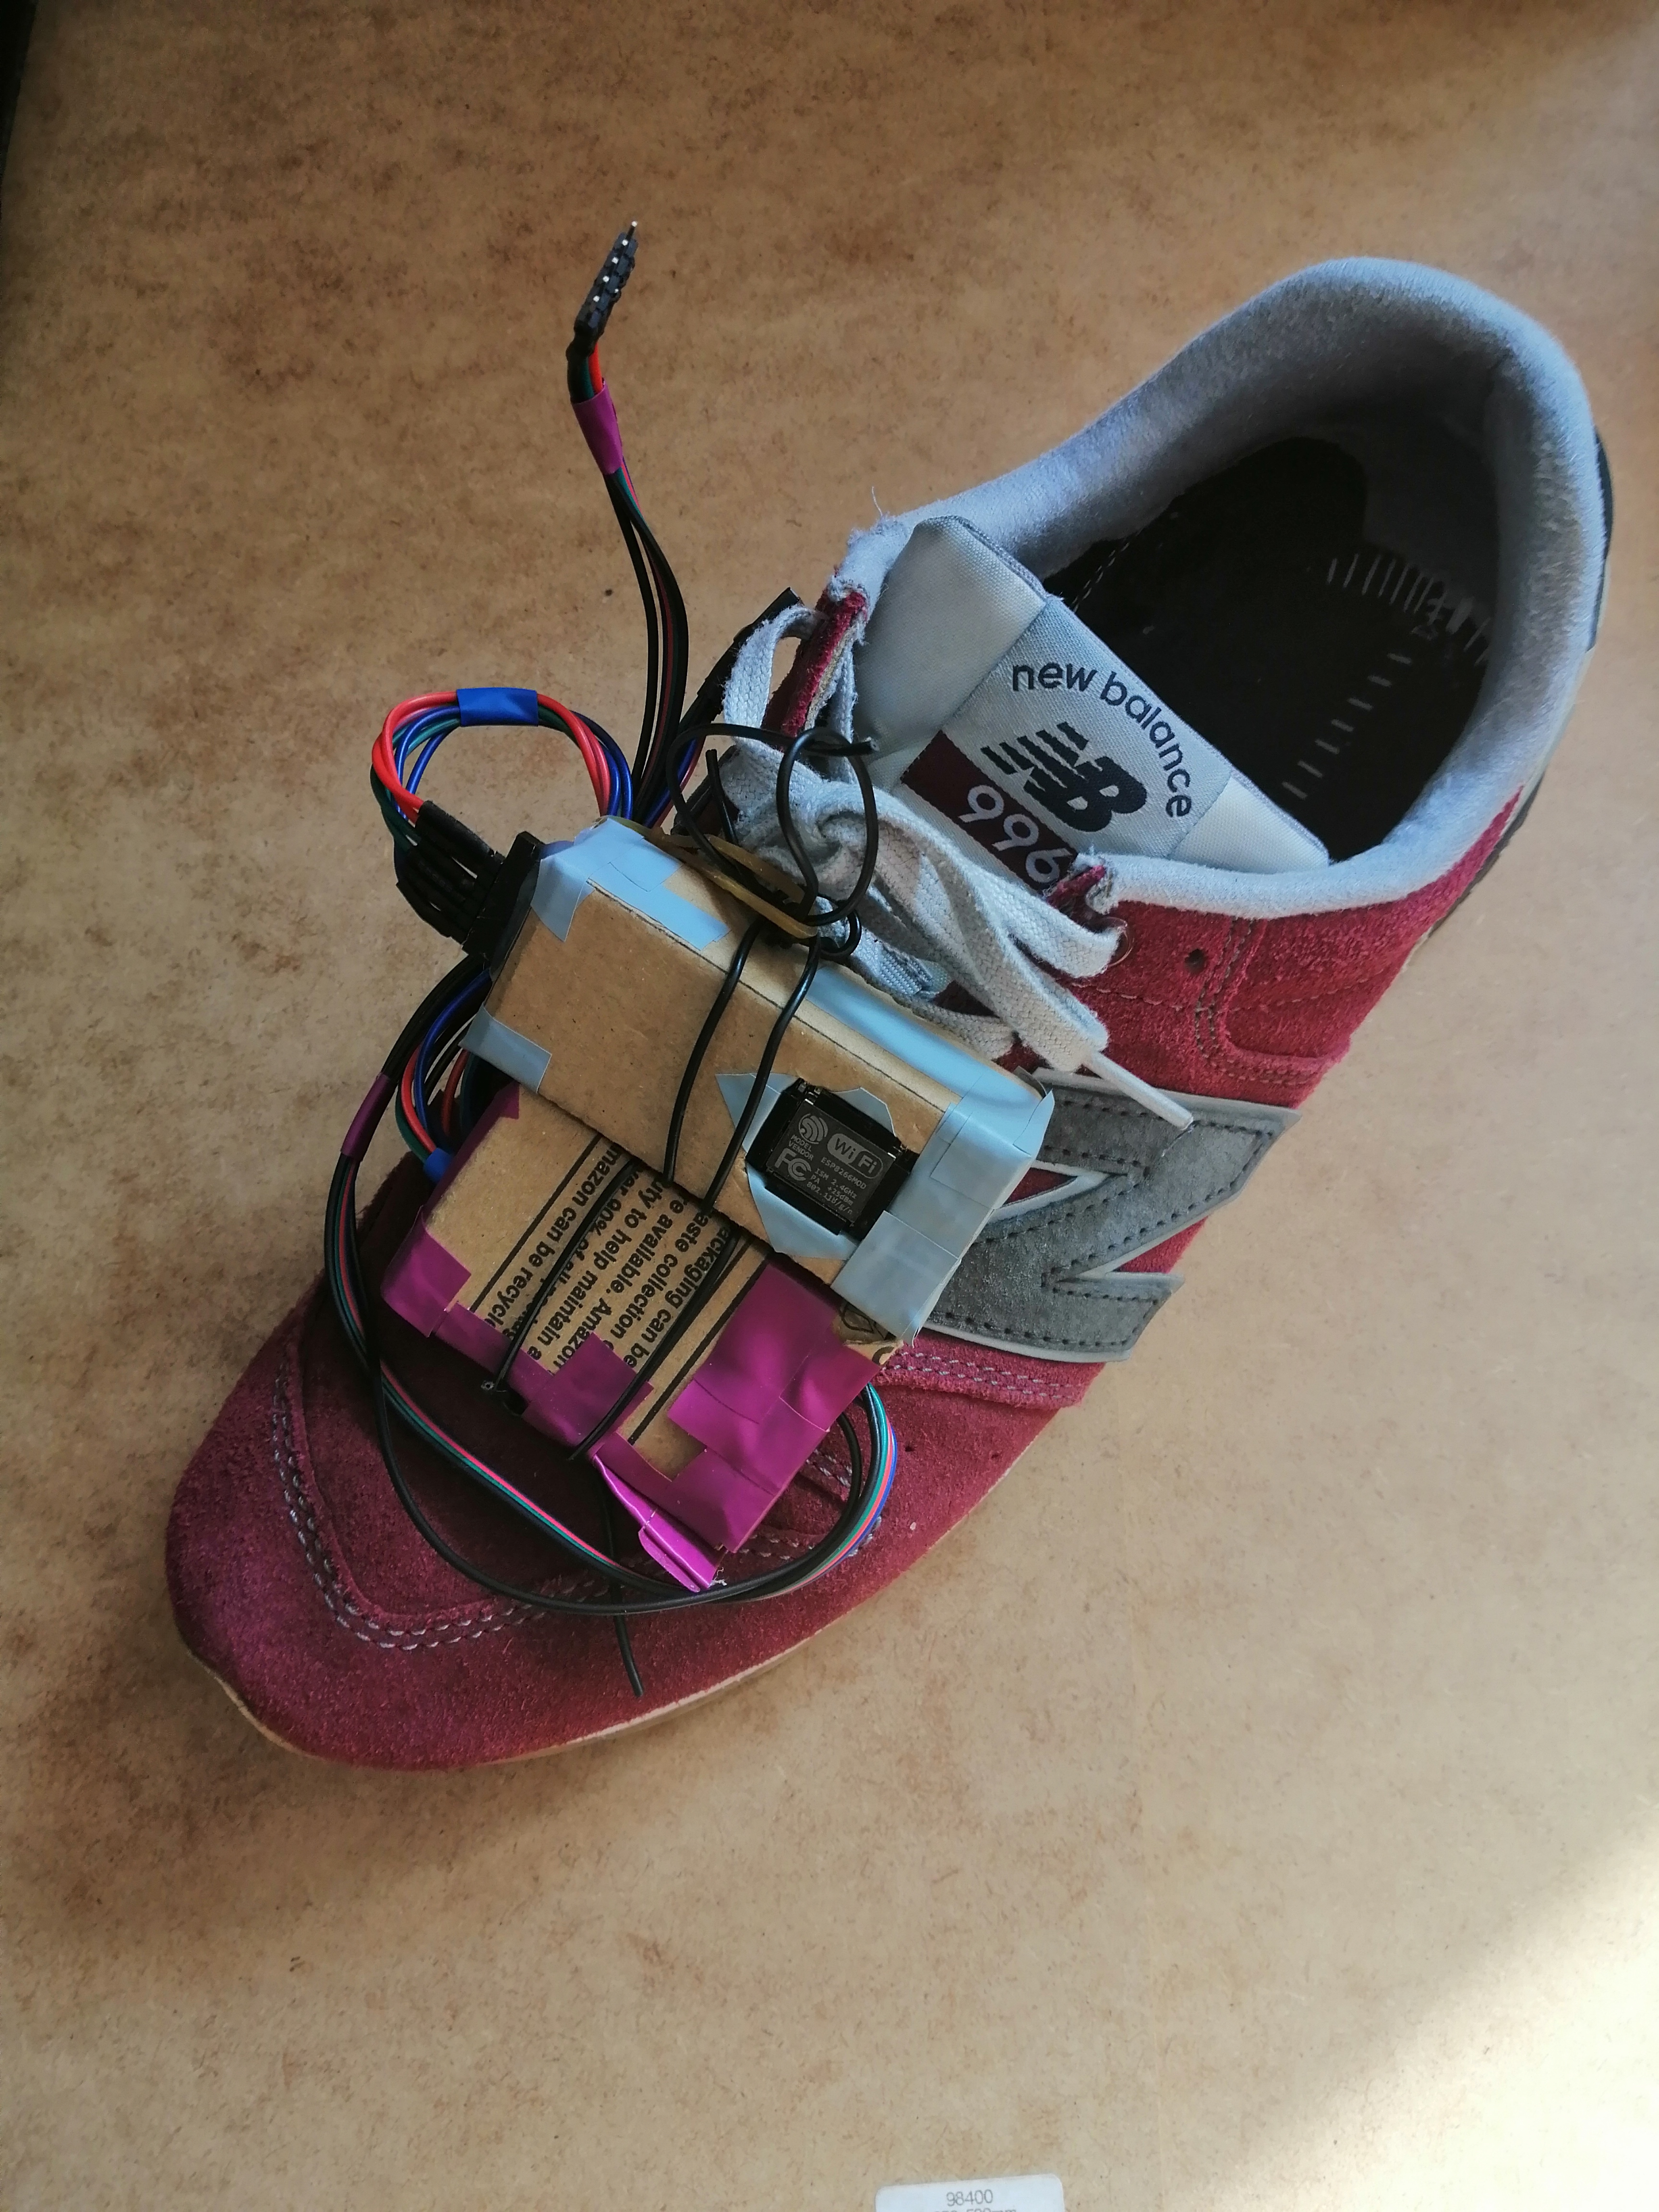
\includegraphics[width = 50mm ]{ShoeAssembled.jpg}
\hfill
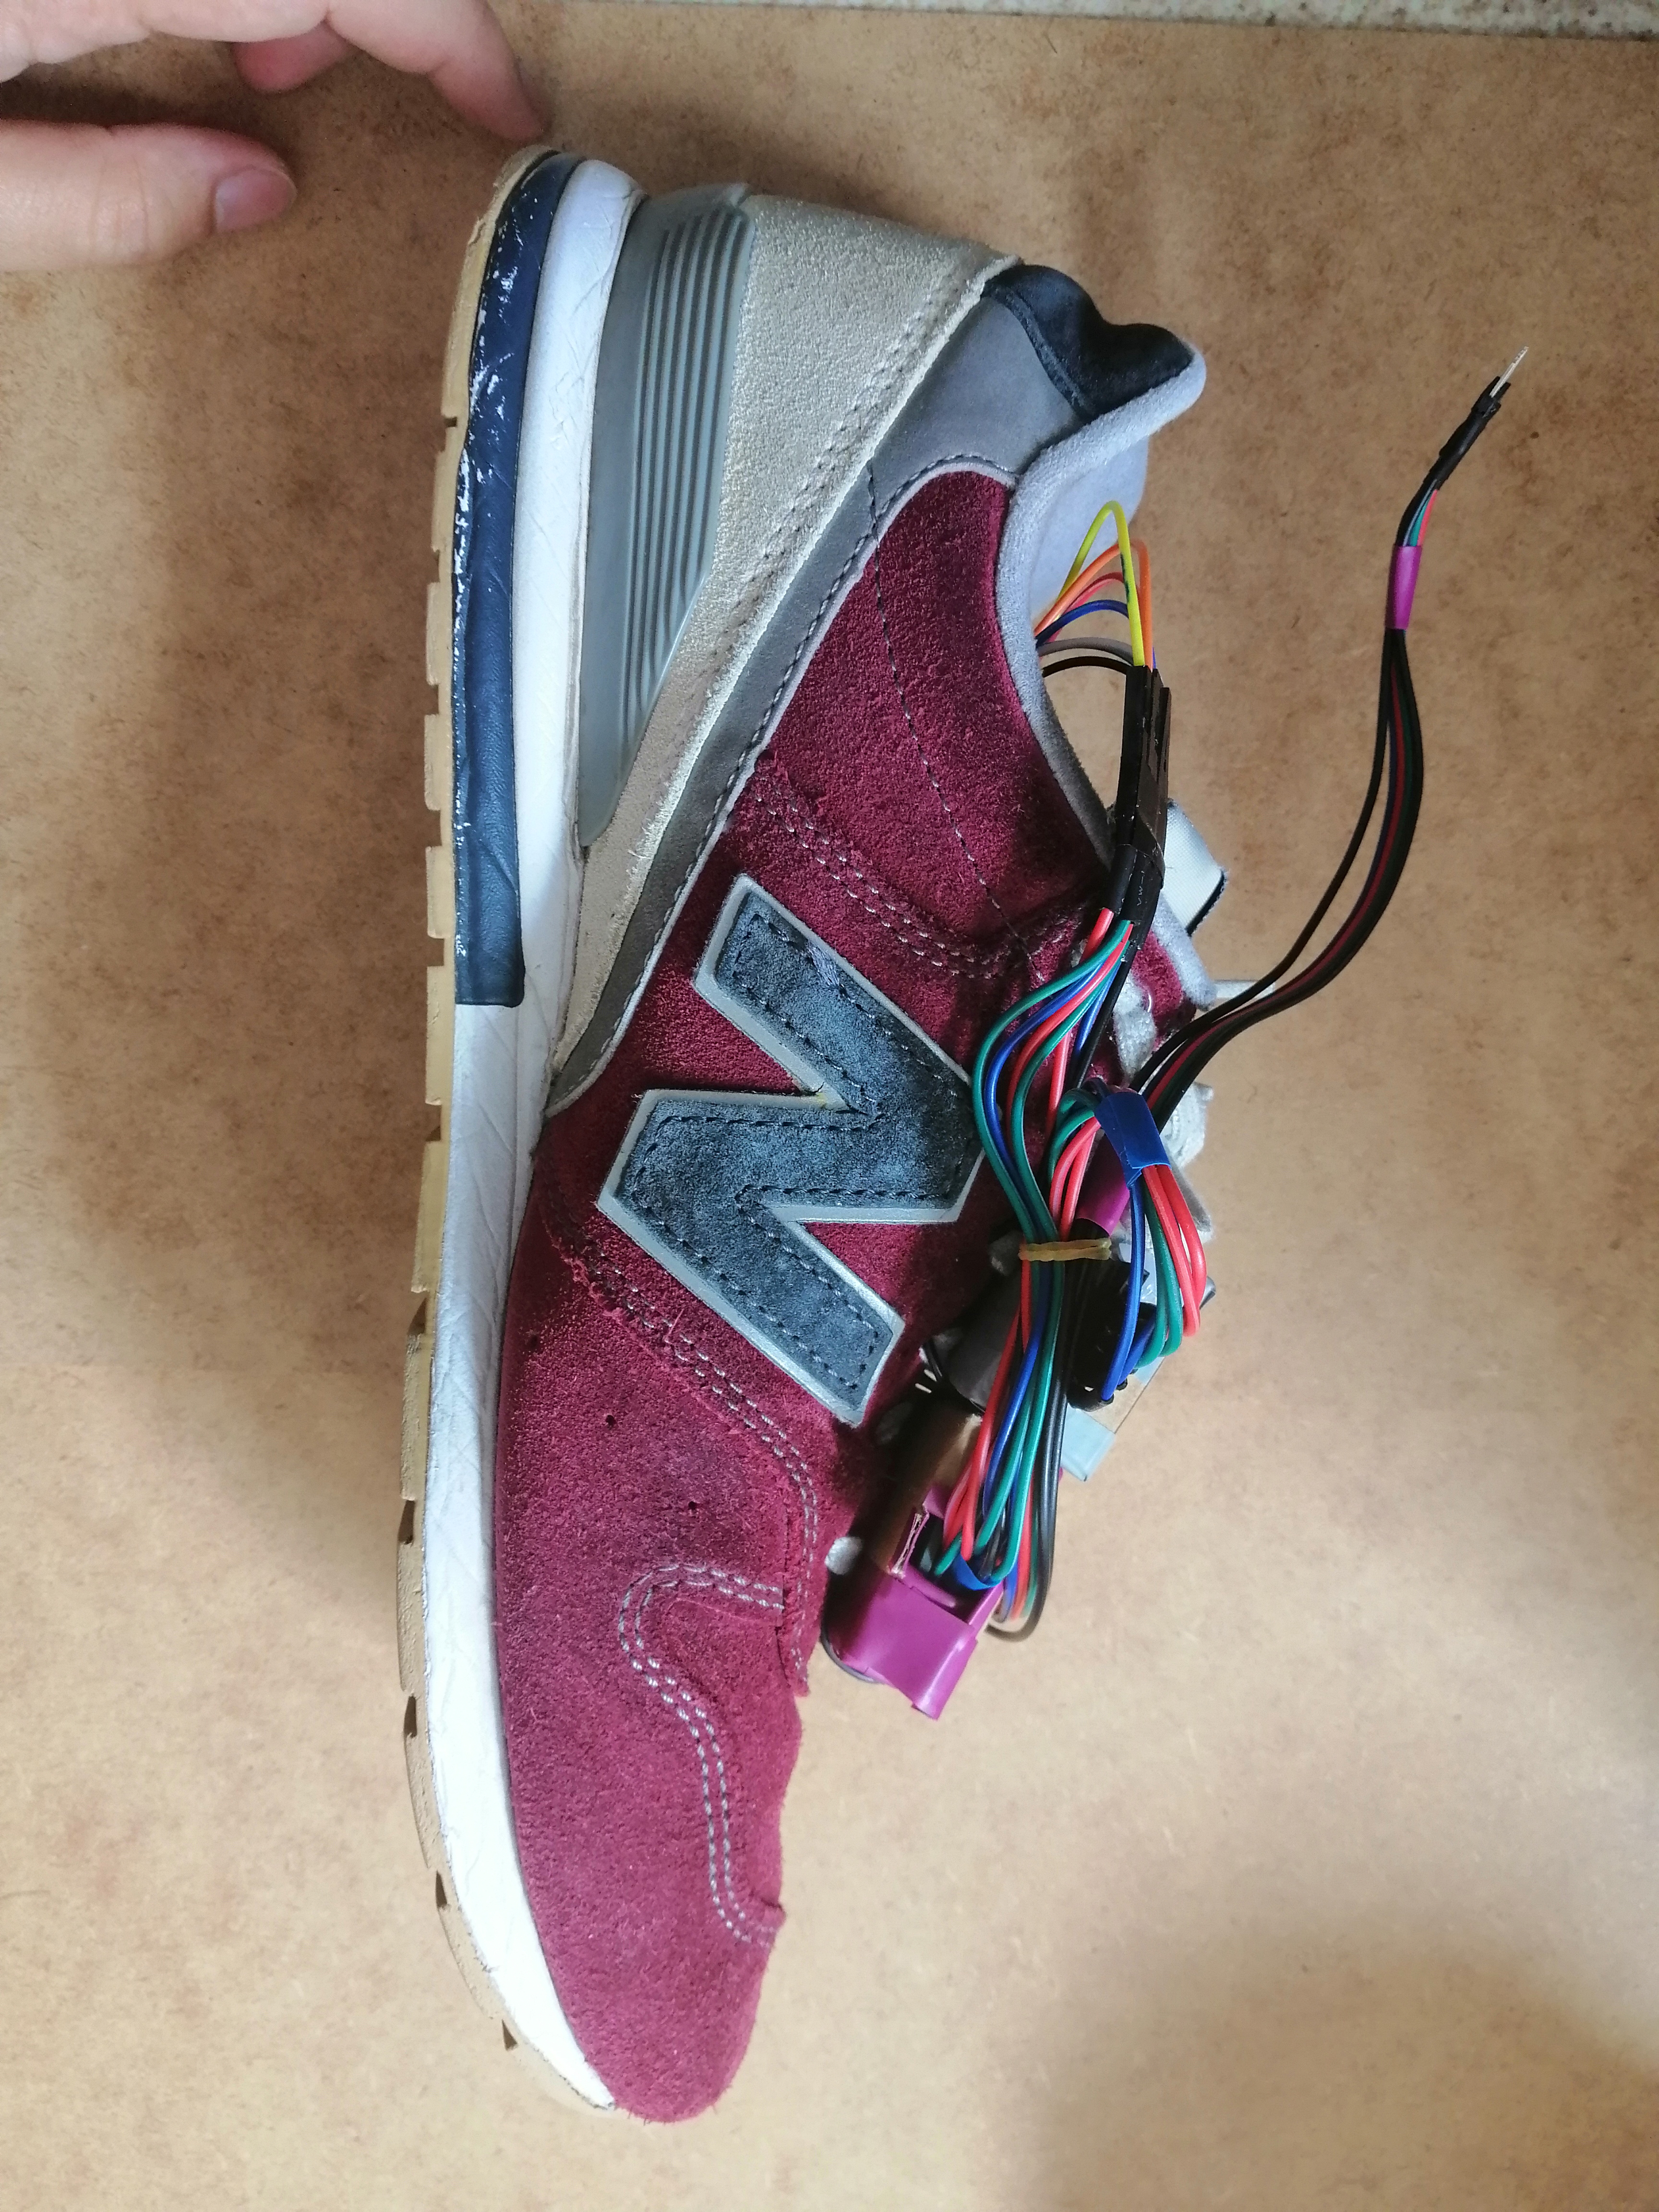
\includegraphics[width = 50mm]{ShoeAssembled4.jpg}
\hfill
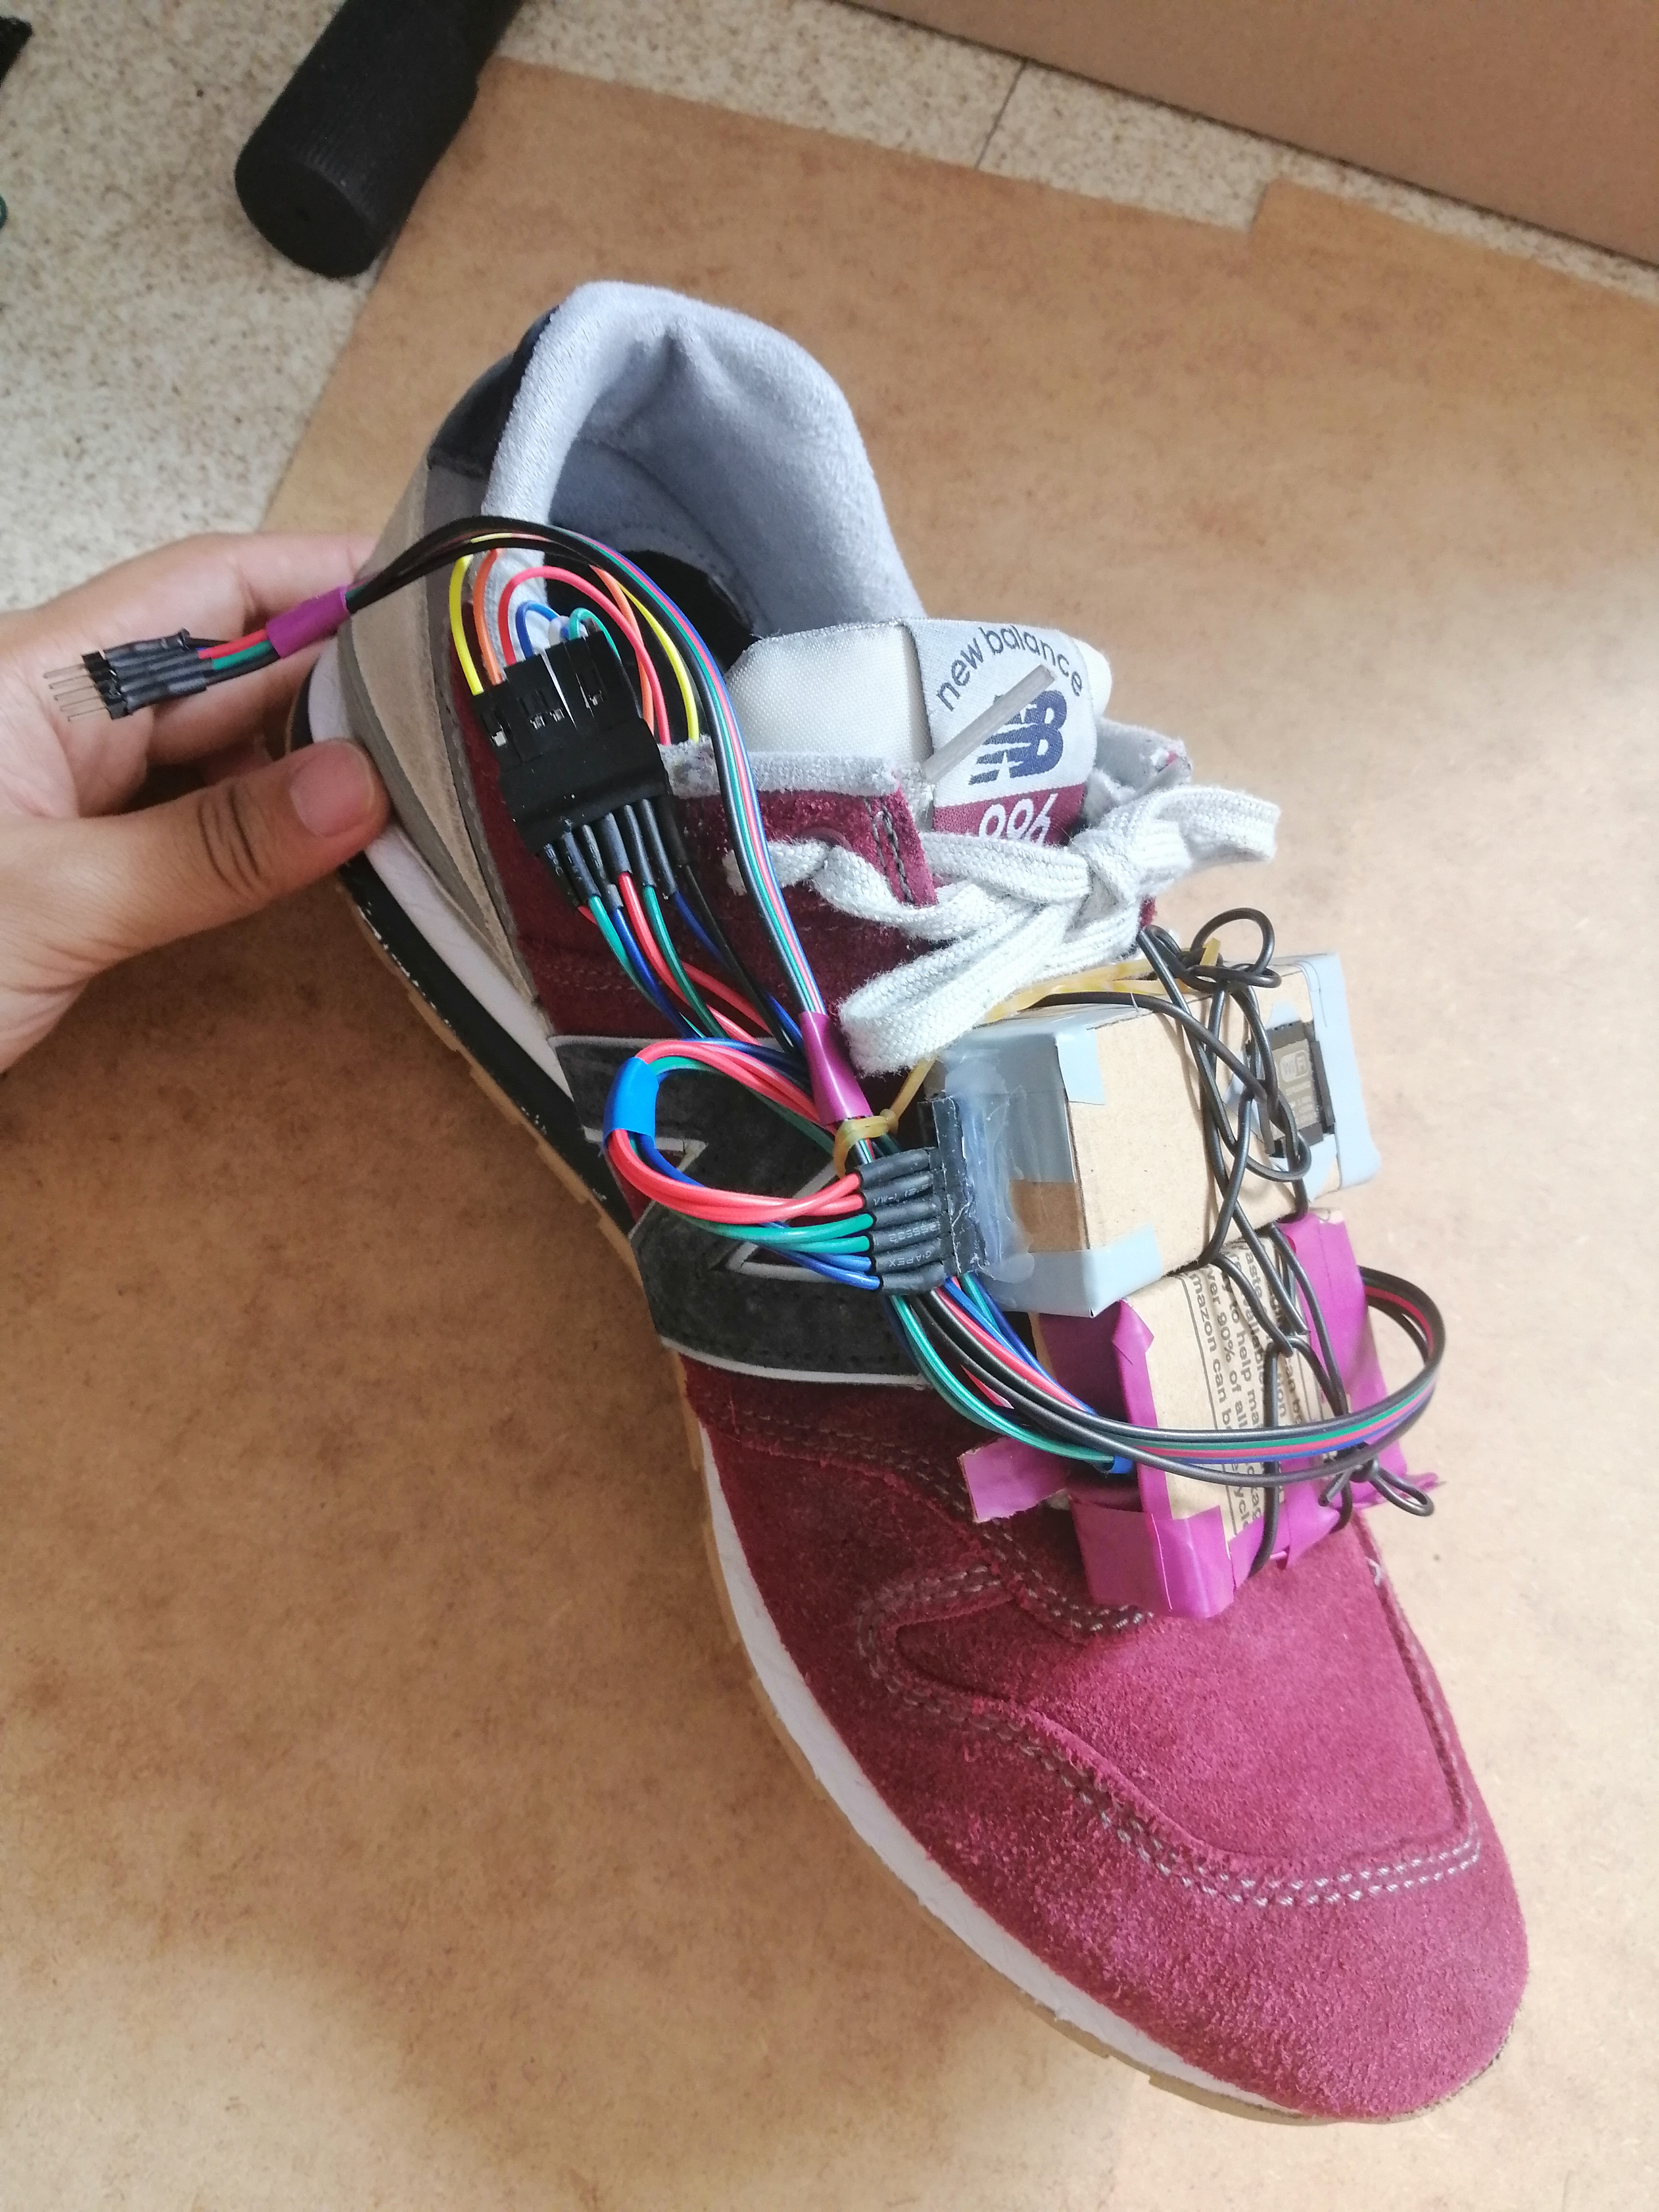
\includegraphics[width = 50mm]{ShoeAssembled3.jpg}
\caption{Shoe assembled with Data Board, Force Board and the insole}
\end{figure}   
\begin{figure}[hbt!]
\centering
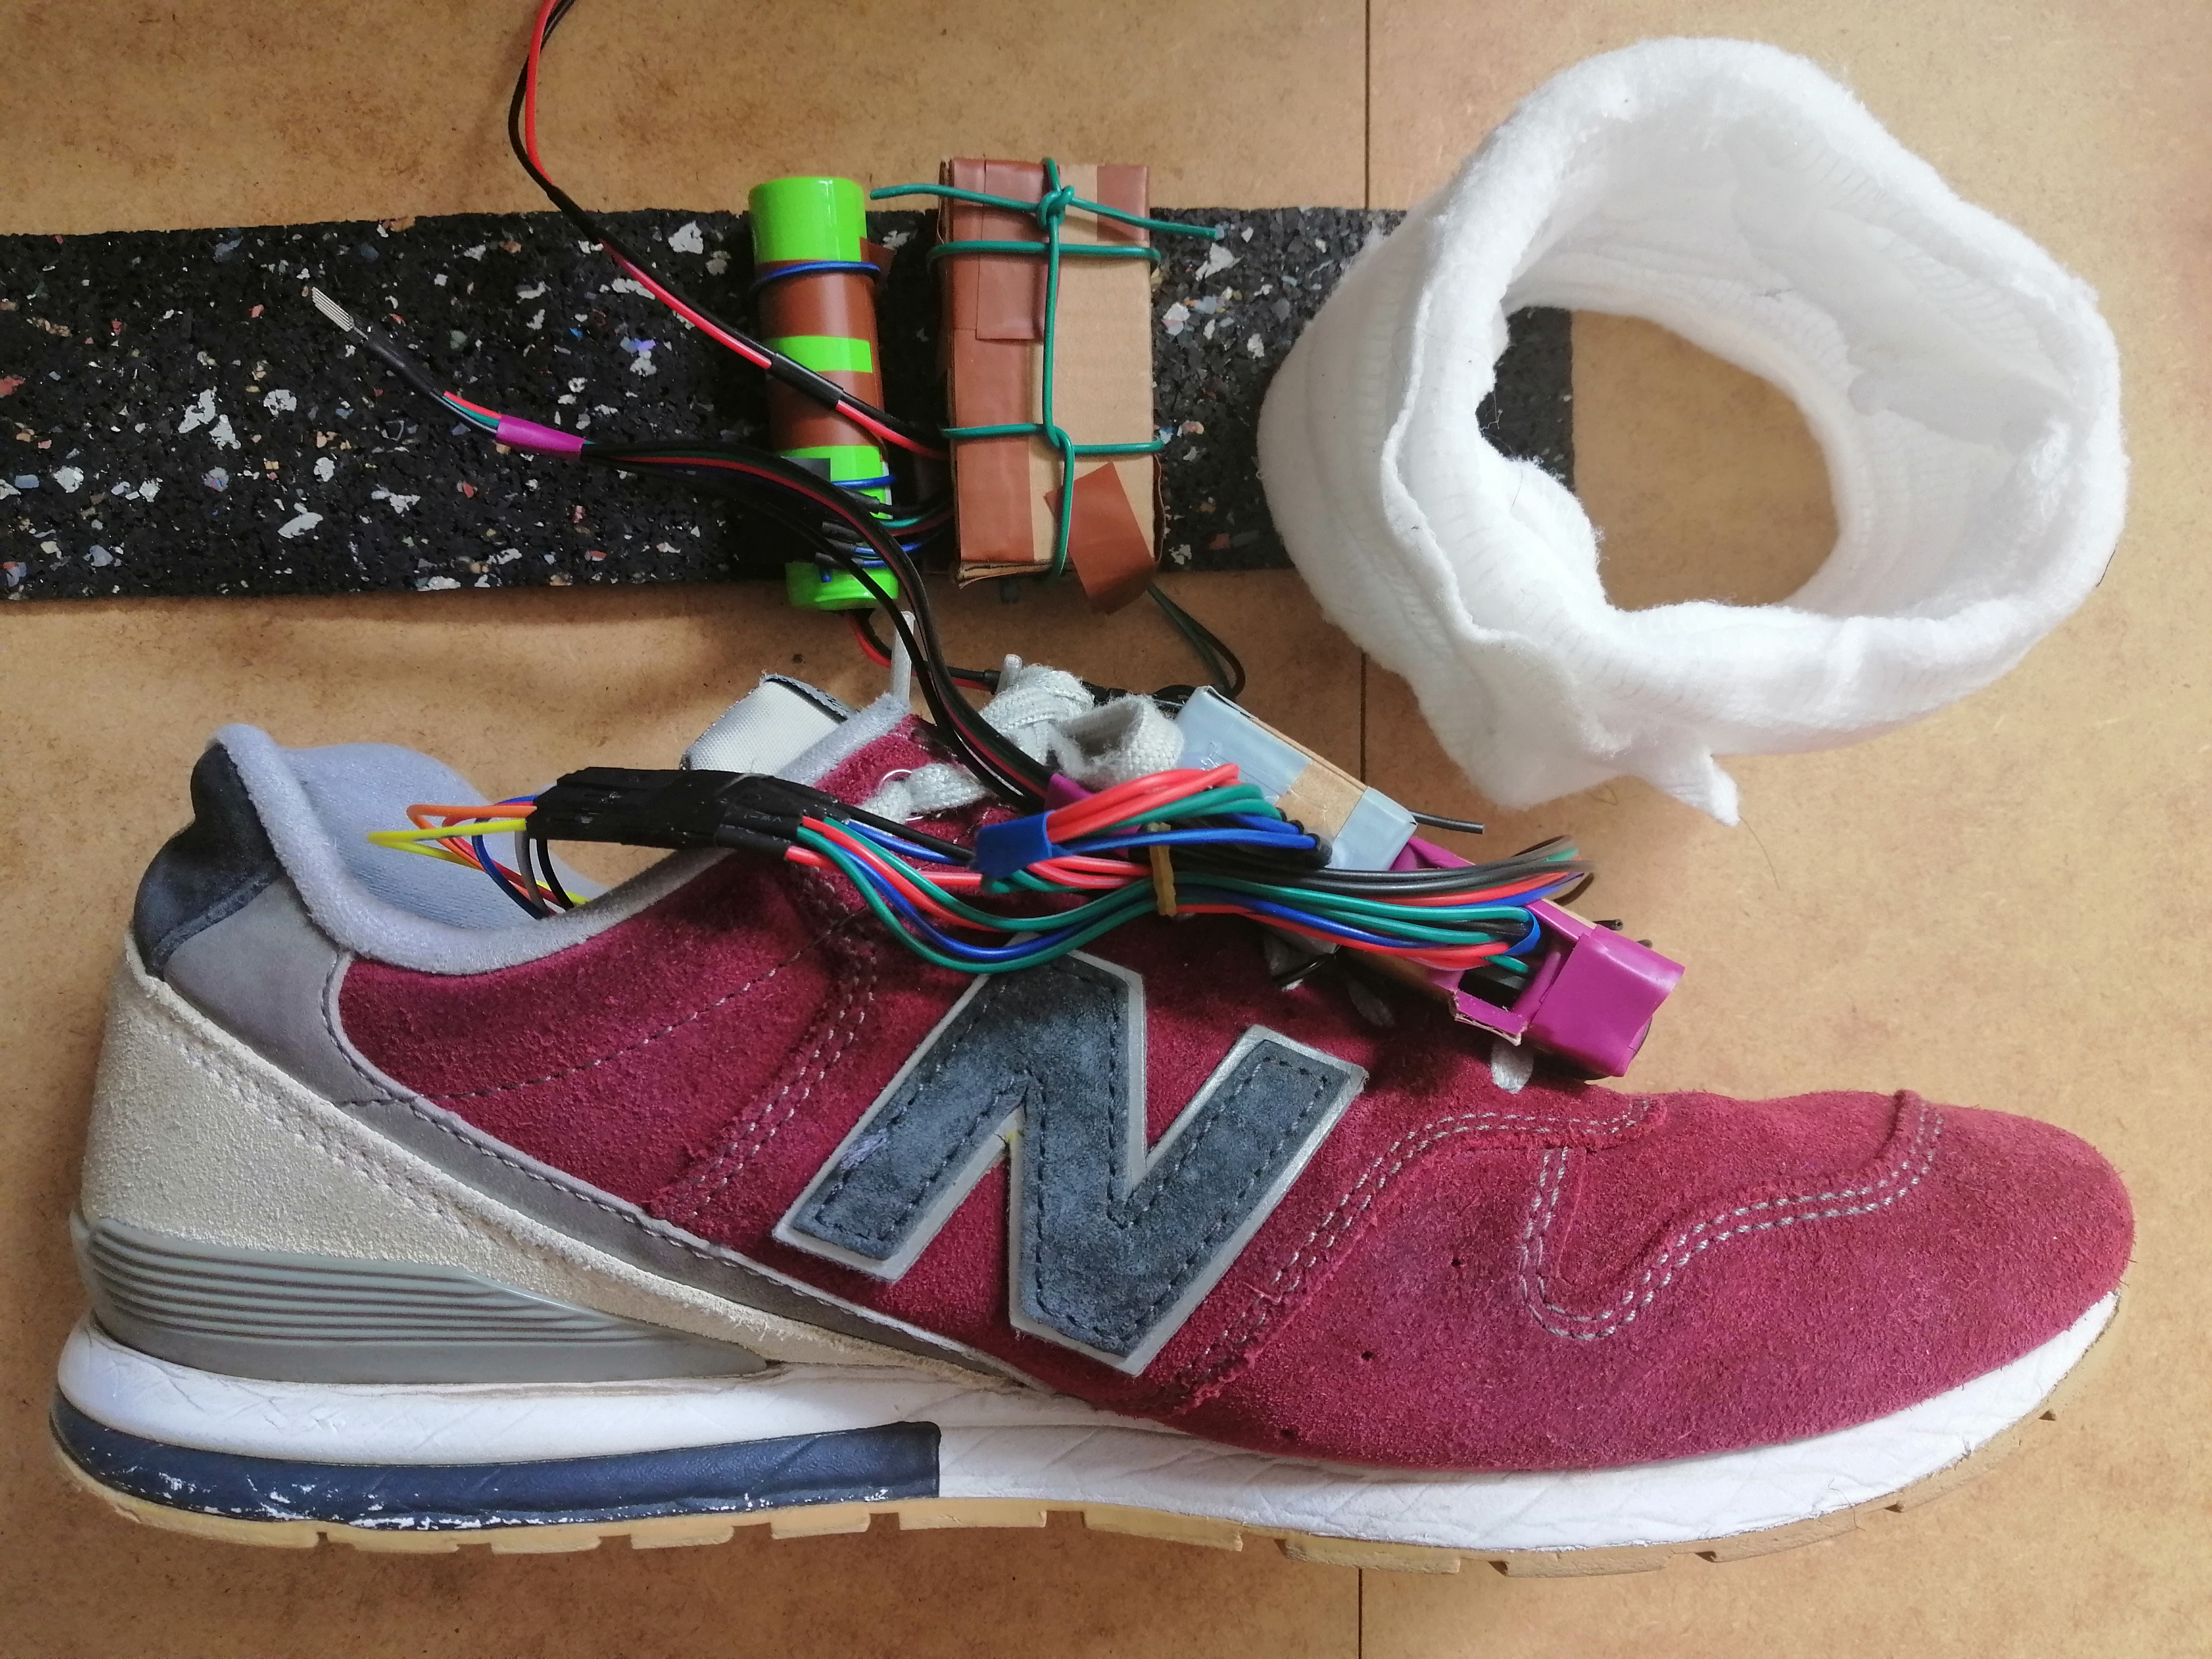
\includegraphics[width=140mm]{AllSystem.jpg}
\caption{All system before wearing}
\end{figure}
\section{Software}
The code can be found with the project, or on the git hub domain at https://github.com/Noath2302/Sensor-Shoe-Project with most of the work done in 	
The Software part include two programs : one on the Esp8266 (sender) and one on the Laptop(PC machine) (receiver). The setup for the software operation requires a LAN (Local Area Network) on the receiver (laptop).
\subsection{Sender}
The sending program has 3 operations : Setup, Collecting data and Sending. As mentioned earlier, the data includes Force Sensing, Acceleration and angular velocity. Additional data that are included are time stamps and time interval. The reading of ADS1115(Force sensing data) and the MPU9250 (Accelerometer and Gyroscope) were made possible by use of Arduino Library: Adafruit ADS1X15 and Bolder Flight Systems MPU9250. The Esp8266 also employ the usage of ESP8266WiFi.h (aware of the letter case) for communicating between the Esp8266 and the server through Wifi. The code of two data input modules(MPU9250 and ADS1115) were separated into two parts: Setup and read. The setup parts set up the I2C connection between the modules and the Esp8266. The Read part read the data from the modules and appends it to the String message through 2 variables "adc" and "imu". The variables were then sent to the loop to combine with time stamp and time interval to become the message. This message would then be written to the socket between esp and the receiver.\\
\begin{figure}[hbt!]
\centering
\includegraphics[scale=1]{messagesender}
\caption{Message that was sent to the server}
\end{figure}
However, the anatomy of the message is a bit special for this design. During testing and measuring time stamps, it was recognized that most delays lies in the reading of the modules, not the Wifi medium. So a data structure was made to combine messages of different time stamps before sending was made.\\
\begin{figure}[hbt!]
\centering
\includegraphics[width = 120mm]{message_sender.png}
\caption{Message anatomy from the client program}
\end{figure} 
dummy string, currently "Z", was put at the end of individual messages before combining. The dummy string act as a marker for the server to separate the data block and get data for each time stamps. This has the advantage that the processing and server code does not need to apply concurrency programming for fast processing. Furthermore, the length of the combined message can also be altered to fit for different design, for example more complex algorithm that requires more time to run.   
\subsection{Receiver}
The Receiver program was currently written in Python. The Program job includes setting a TCP/IP Socket connection with the Esp over the hosted LAN, process received the data and process in real time. It was tempting to use terminology as concurrency for such processing job. But by current design, most of the bottle neck in the Sensor-Shoe system lies on the reading of data. So every time the Esp has done the send data process, and send them effortlessly, the Receiver has at least 60ms for processing.This is already a lot of time for the data to be processed.\\
Current work done by the processing code:
\begin{itemize}
\item{separate the message to time stamp data}
\item{real-time plot the data}
\item{use python code on the smart phone, this requires manually detecting the code and upload to the system}
\end{itemize}
The Receiver first open a Server Socket on the host machine, by combining the host ip and the port. This socket then start listening for the connection from the client socket. After the connection have been established, the server start receiving message from the client, or the Esp8266 through the socket. The Server then proceed to check for the "END" String in the message. If the string is found, the server stop and the program ends. This can only be triggered once every program run time.\\
The message was then processed by function \emph{ListSplit()}. This function exploit the usage of the "Z" marker in the section of the sender. The return output then become a list of float vector each vector contains 13 entities: 6 force sensor data + time stamp + 3 acceleration + 3 angle velocity.\\
\begin{figure}[hbt!]
\centering
\includegraphics[width = 120mm]{messageReceiver.png}
\caption{ return List after "Z" extraction from messages}
\end{figure}
\\
The returned List is then added to a dataStream, this dataStream holds the data List to a certain number of vector point, control by constant n = BLOCKSTREAM (currently set 120 point). This stream avoid the program to take too much data, making an "infinite number of elements" List. Initially when the data point received is smaller than BLOCKSTREAM, the dataStream keeps adding the data from the message. After the count of data point exceed BLOCKSTREAM, the function to update dataStream runs another job to delete the old, or stale data from the Stream, releasing space for fresh, new data point, Fig. 3.29.
\begin{figure}	
\centering
\includegraphics[width=120mm]{messageReceiver2.png}
\caption{dataStream update data point}
\end{figure}
\\
The dataStream acts as a buffer for the processing code to iterate through. Before that, It can also be plotted to see the real time behavior of the system when walking. To plot the dataStream, another function was written to extract the respective data dimensions into separated List with same index point. Briefly, It is like transposing a matrix of dataStream, from having n 12d- vector to having 12 data vectors of n time stamps. Then the vectors were plotted with respect to time and update by repeatedly refreshing dataStream content.
\begin{figure}[hbt!]
\centering
\includegraphics[width=120mm]{dataPlot.png}
\caption{transposed version of the data to plot}
\end{figure}
\\After done the code the data can be plotted in real time. The current plotting API is matplotlib.pyplot from python, the usage and implementation of the code can be found on matplotlib official documentation. Fig. 3.31 shows a sample walking pattern plotted down on the window(4 steps).
\begin{figure}
\centering
\includegraphics[width = 140mm]{walking.png}
\caption{Real time plot running when walking}
\end{figure}
\subsection{Processing code}
The processing part hadn't been realized in time for the testing and data collection of the work. However, a small section is kept here for idea and reference for ones who wish to continue, as further work on this project.\\
The goal of processing code isto recognize walking data on ground level vs climbing a stair. To achieve this, the processing code was put to iterate over the dataStream every time the Server receive data. The recognition is done by first recognizing the gait cycle. Then each gait cycle would be normalized to the same length of a sample gait cycle. Considering each gait cycle at this time is a multi-dimensional vector. Vector distance between the analyzing cycle and the sample cycle will determine if the cycle is classified as walking or climbing stair.\\
Another remark to calculate vector distance is that there are  different values: voltage, acceleration and angular velocity. To not change or develop a specific gain for each and sum up, The 3 different distance value are kept. Consequently, a 3d- distance vector was used for the recognition. The recognition was done by putting a 3d threshold vector, if the distance vector exceed the threshold, it is not recognized.\\
The Sample gait cycle was achieved by manually seeing and marking the data after each data collecting course. The data was written to a file everytime the program ends.
\begin{figure}[hbt!]
\centering
\includegraphics[width = 120mm]{writeFile.png}
\caption{Code piece for writing dataList to the file}
\end{figure}
The data was not added in the loop to periodically append the data to the file. This was done to avoid faulty situations that can corrupt the data. The code was put at the end of the file, to make it run only if everything else was good. In the other hand, the code was only put for the finding of a sample gait cycle. In longer run for example 30 minutes, this code should be omitted to save list variable dataList from overloading and slow the program.\\
The analysis were meant to be done in Excel. After having identified the good gait cycles, the sample gait is set by taking the average of the selected gait.\\
\chapter{Result}
\begin{figure}[hbt!]
\centering
\includegraphics[width=140mm]{shoe2.jpg}
\caption{SensorShoe system when installed in the foot area}
\end{figure}
The System has been realized with 3 board + 1 insole setup. All can be installed on the left shoe during operation. Although the system was not comfortable to wear, the hardware rarely affected the inspected gait.\\
A real time plot has been made to visually observe the data. With the aid of this, some knowledges from gait analysis and time, an gait-recognition processing function could probably be carried out.\\
\section{Real Time Plot}
The current setting for the system:
\begin{itemize}
\item{sender send a 3 12d-vector combined message}
\item{dataStream holds 120 data points}
\item{host ip : 192.168.137.1 (local host on LAN),it is recommended to use static ip}
\item{port: 22222, should be larger than 10000 to avoid reserved ports}
\item{take 30 sec data collection, count since the first data transfer, not including setup time}
\end{itemize}
All of the above elements could be changed from altering the code.
\chapter{Discussion}
\section{Hardware}
\subsection{Design}
As stated earlier this project acts rather as a complete prototype test than a final product. The board was intentionally separated to reduce risk of failures and permits ease with independent board testing. It took more time to make 3 boards, but should have saved a lot of time for debugging and tweaking the system. As for the lack of time, not many boards were manufactured for more test.\\
The PCBs were not made by the same manufacturer, which cost more time in the working routine. The design should always be checked carefully before manufacturing, for isolation, placement of device, route width, drills and alignment. Back to this project, many other researches in the alike system developed a compact, all-in-one design that contain everything\cite{Shuo}\cite{Kim}\cite{Nilsson}. So one good direction to improve the system is to put everything in one device and replace the used of development board with their respective circuit in the design. This will for sure make the design more dense to match the wearable dimension on the foot. The approach also keep the system from physical disturbances e.g wired electrical connection between interfaces and wires themselves.\\
The design could also use a smaller battery. For the current 18650 hasn't even been charged during the whole working time of the thesis and still working. An earlier work on the project had pointed out the working capacity for 160 minutes to be around 228.26mAh. And batterey such as 400mAh-800mAh would be suitable for the system to be powered. A 18650 with 2200mAh is an overkill thus expose the system to a risk of rather high current, which did kill some IC during the prototyping period of this thesis. Weight was also a factor to considered for natural gait data (a 18650 weighs around 45g)\\ 
\subsection{Manufacturing}
A good practice for the writer when designing and working with the PCBs is patience\footnote{This part was added by the writer so that ones can avoid the now foreseeable mistakes}. Engaging in testing and working can be very tempted. Thus such haste at this point  also expose the worker to the error-prone decision. Care and thoughtfulness are the main key in testing a circuit, it was better a little late than to do it all over again.\\
Problems encountered:\\
The Power board burned the LMV324 on it when a short circuit occurred during the first walking test (I put it in the sock). This caused several copper tracks to be torn out. The solution was to solder the torn tracks with an additional small copper wiring (extracted from a flexible copper wire) and replace the LMV324. A shielding of hot glue was then applied to the bottom of the board for insulation. A carbon container was also applied to provide casing.\\
The Data Board was not fully milled as some drill tracks were still remained on the bottom side. A hand drill was then used by hand to remove the remained copper drill tracks on the board.\\
The Force Board had one pin that wasn't soldered, this was due to the lack of solder paste during the SMDs installment before going through oven. This was found in shoe installment section, as one of the force sensors didn't behave like others. Fixed by hand soldering the pin.\\
The VHIGH wire from the Power Board to the Data Board was torn because of colliding with the right shoe. Occurred during durability test to the supermarket.\\
\section{Software}
\subsection{General}
During the operating of the system, the roll of network interference is also quite high. The device was detected to not sending some data, which cause the crash in the system. This usually occur when turn on the system for the first time as the switching cause some unexpected voltage spikes. This somehow make the wifi operation of the esp8266 distorted and send malicious message and stop system operation. The Script usually ends with out of index of list error, this is due to the missing of one data point in the awaited data array. The current solution for this unpredictable data is to proof force the missing data by replacing it with a medium of neighbor ones. A small delay of 1-2 seconds between connection code and data transmission is also applied to seclude the transmission from the power spike.\\
\\
The current design also suffers from distance, when the wearer goes to far from the host. The sending of the signal become corrupted, the message usually halved or some negative sign \"-\" that cannot be transformed to float value. Either way, the program broke with exception. These are to mention the dependency of the transmission on the Wifi medium and the environment.  
\subsection{Python Script:}
Due to the limited time, Python was chosen to be the programming language of the project, due to its feasibility. The project also considered c++ and Java before as they are more reliable and indeed faster. C++ socket however was hard to implement and was dropped during the working time of this thesis. Java was formerly the working server and was used repeatedly to test the client side(Esp8266). Further works can include changing the approach of programming language. Python is a good choice, since it boosted up the working process. But it also made the coder comes with a lot of abundant code when in haste. A fast work may include cleaning up the code and its logic, to reduce abundance of array iteration.\\

As discussed from above, despite the fact that this is a real-time system, there hadn't been a need for concurrency programming. Further works may include adding concurrency logic to the processing part of the code. AsyncIO was first considered to the code. The basic of this API is that it manage a pool of tasks. During each task runtime, the task will stop at some point when executing and wait for some other task to complete or for a timed period. When all the task changed to wait, the task with the longest wait time will run first, then so on. For our system, to demonstrate, can have 2 tasks: to collect data and to process data. The processing task run and wait for the collecting task to return the data. The collecting task then wait for the processing task to return a trigger that the processing of the data is done. This should be more sensible if a system of multi processing-collecting tasks can be realized from the system. For example: data transfer in different ports or separated reading of each data types at a time. 

The Python script (Python3) was also set to run on a Android smartphone. The phone hosts a server, and run the data collecting script beautifully, using PyDroid app on Android. The only problem was that the phone host ip changed every time it turn on the hotspot. This left space for some configurations before a run on the system could be deployed. The code at this point can be further improved to fix this problem. One way to do this is to host the serer on the Esp8266 and let the PC machine (laptop and smartphone) to act as a client. This can avoid the risk of having random ip on phone, thus keep the Esp8266's ip static.
\chapter{Conclusion}
The Project didn't get to the intended goal made in the beginning, there are still a lot of intention and idea that can be extended and considered. However it has provided a lot of working experience and learning during the period. The data was plotted and react with respect to foot motion. The periodic representation of the plot also resemble the steps, or gait cycles when walking. 
To sum up, this project has provided a design for collecting gait data and a way we can use to process it to get the desired output. The prototype has the combination of all common inputs from the foot area by the time written. The system was not a final design but can generate good data for further processing or test data set for applications of different processing method.   
%===================================================================
\begin{thebibliography}{99}
\bibitem{silverA301}
Tekscan, “How Does a Force Sensing Resistor (FSR) Work?” www.tekscan.com/blog/ flexiforce, Jul. 03, 2019. [Online]. Available: https://www.tekscan.com/ blog/ flexiforce/ how-does-force-sensing-resistor-fsr-work. [Accessed Aug.04, 2019]
\bibitem{lmv324}
STMicroelectronics, "Low cost, low power, input/output rail-to-rail operational amplifiers," LMV324 datasheet, Oct. 2015 [Revised Aug. 2019]
\bibitem{diy}
diymodules.org, "Download Files", Eagle Lib file download, Available: https:// www.diymodules.org/ download/ eagle-libs/ dm/ diy-modules.lbr. [Accessed Aug.05, 2019]
\bibitem{tekscan}
Tekscan "Why is Gait Analysis Important?" https://www.tekscan.com/blog/medical, Jan 02 2018.[Online]. Available: https://www.tekscan.com/blog/medical/why-gait-analysis-important [Accessed Aug.21 2019]
\bibitem{whittle}
Levine, David \& Richards, Jim \& MW, Whittle. (2012). Whittle$'$s Gait Analysis
\bibitem{katzen}
Pirker, W., \& Katzenschlager, R. (2017). Gait disorders in adults and the elderly : A clinical guide. Wiener klinische Wochenschrift, 129(3-4), 81–95. doi:10.1007/s00508-016-1096-4
\bibitem{protokinematic}
Protokinetics Team, "Understanding Phases of the Gait Cycle", https://www.protokinetics.com Nov. 28 2018. Available:  https://www.protokinetics.com/2018/11/28/understanding-phases-of-the-gait-cycle/
[Accessed Aug. 22 2019 ]
\bibitem{gaitcycle}
Uustal, H.; Baerga, E. Physical Medicine and Rehabilitation Board Review; Demos Medical Publishing: New York, NY, USA, 2004.
\bibitem{Monaghan}
C.Monaghan, W. van Riel and P. Veltink, "Control of triceps surae stimulation based on shank orientation using a uniaxial gyroscope during gait", Medical \& Biological Engineering \& Computing, vol. 47, no. 11, 2009. Available: 10.1007/s11517-009-0539-8 [Accessed 27 August 2019].
\bibitem{Kim}
D. Lim, W. Kim, H. Kim and C. Han, "Development of real-time gait phase detection system for a lower extremity exoskeleton robot", International Journal of Precision Engineering and Manufacturing, vol. 18, no. 5, pp. 681-687, 2017. Available: 10.1007/s12541-017-0081-9 [Accessed 27 August 2019].
\bibitem{Zhang}
C. Zhang, X. Zang, Z. Leng, H. Yu, J. Zhao and Y. Zhu, "Human–machine force interaction design and control for the HIT load-carrying exoskeleton", Advances in Mechanical Engineering, vol. 8, no. 4, p. 168781401664506, 2016. Available: 10.1177/1687814016645068.
\bibitem{Mohamed}
M. Mohamed Refai, B. van Beijnum, J. Buurke and P. Veltink, "Gait and Dynamic Balance Sensing Using Wearable Foot Sensors", IEEE Transactions on Neural Systems and Rehabilitation Engineering, vol. 27, no. 2, pp. 218-227, 2019. Available: 10.1109/tnsre.2018.2885309 [Accessed 27 February 2019].
\bibitem{Shuo}
S. Ding, X. Ouyang, T. Liu, Z. Li and H. Yang, "Gait Event Detection of a Lower Extremity Exoskeleton Robot by an Intelligent IMU", IEEE Sensors Journal, vol. 18, no. 23, pp. 9728-9735, 2018. Available: 10.1109/jsen.2018.2871328 [Accessed 27 August 2019].
\bibitem{Nilsson}
J. Nilsson, I. Skog, P. Händel and K. V. S. Hari, "Foot-mounted INS for everybody - an open-source embedded implementation," Proceedings of the 2012 IEEE/ION Position, Location and Navigation Symposium, Myrtle Beach, SC, 2012, pp. 140-145.
\bibitem{ETut}
"OpAmp tutorials", Electronics Tutorials, 2019. [Online]. Available: https://www.electronics-tutorials.ws/category/opamp. [Accessed: 01- Sep- 2019].
\end{thebibliography}
\end{document}
